% ~2-2.5 pages.
\section{Experiments}\label{sec:experiments}



We conduct four experiments to answer the following research questions:
\begin{enumerate}
    \item Does our method outperform state-of-the-art curriculum learning methods on a high-dimensional quadrupedal locomotion task with sparse rewards and long horizons?
    \item Does expanding the curriculum bidirectionally improve sample efficiency and robustness compared to unidirectional expansion?
    \item Does task-space coverage-driven exploration promote more diverse learning outcomes?
    \item Does our method transfer to real-world terrains and tasks, demonstrating its practical applicability and robustness in real-world scenarios?
\end{enumerate}

%TODO: review once we have all experiments

The experiments are implemented in Isaac Lab~\citep{nvidia2025isaaclabgpuacceleratedsimulation} with the ANYmal D quadrupedal agent and the RSL-RL framework~\citep{schwarke2025rslrllearninglibraryrobotics} for training the policy with PPO~\citep{schulman2017proximal}. The following experiments use standard observation and action spaces which are detailed in Appendix~\ref{sec:appendix_obs_act}. The tasks are shown in Figure~\ref{fig:experiment_renders}. The task space $\mathcal{T}$ used for our method's random point sampling and goal definition is a 3D box defined in the $(x,y,z)$ space, i.e., $\phi(s)$ is the projection of the base position to $(x,y,z)$. We found this to be the most effective task space, as it is both convenient for goal definition and provides a simple Euclidean distance metric for the nearest-neighbor search.
\begin{figure}[h]
    \centering
    \hfill
    \begin{subfigure}[t]{0.24\linewidth}
        \centering
        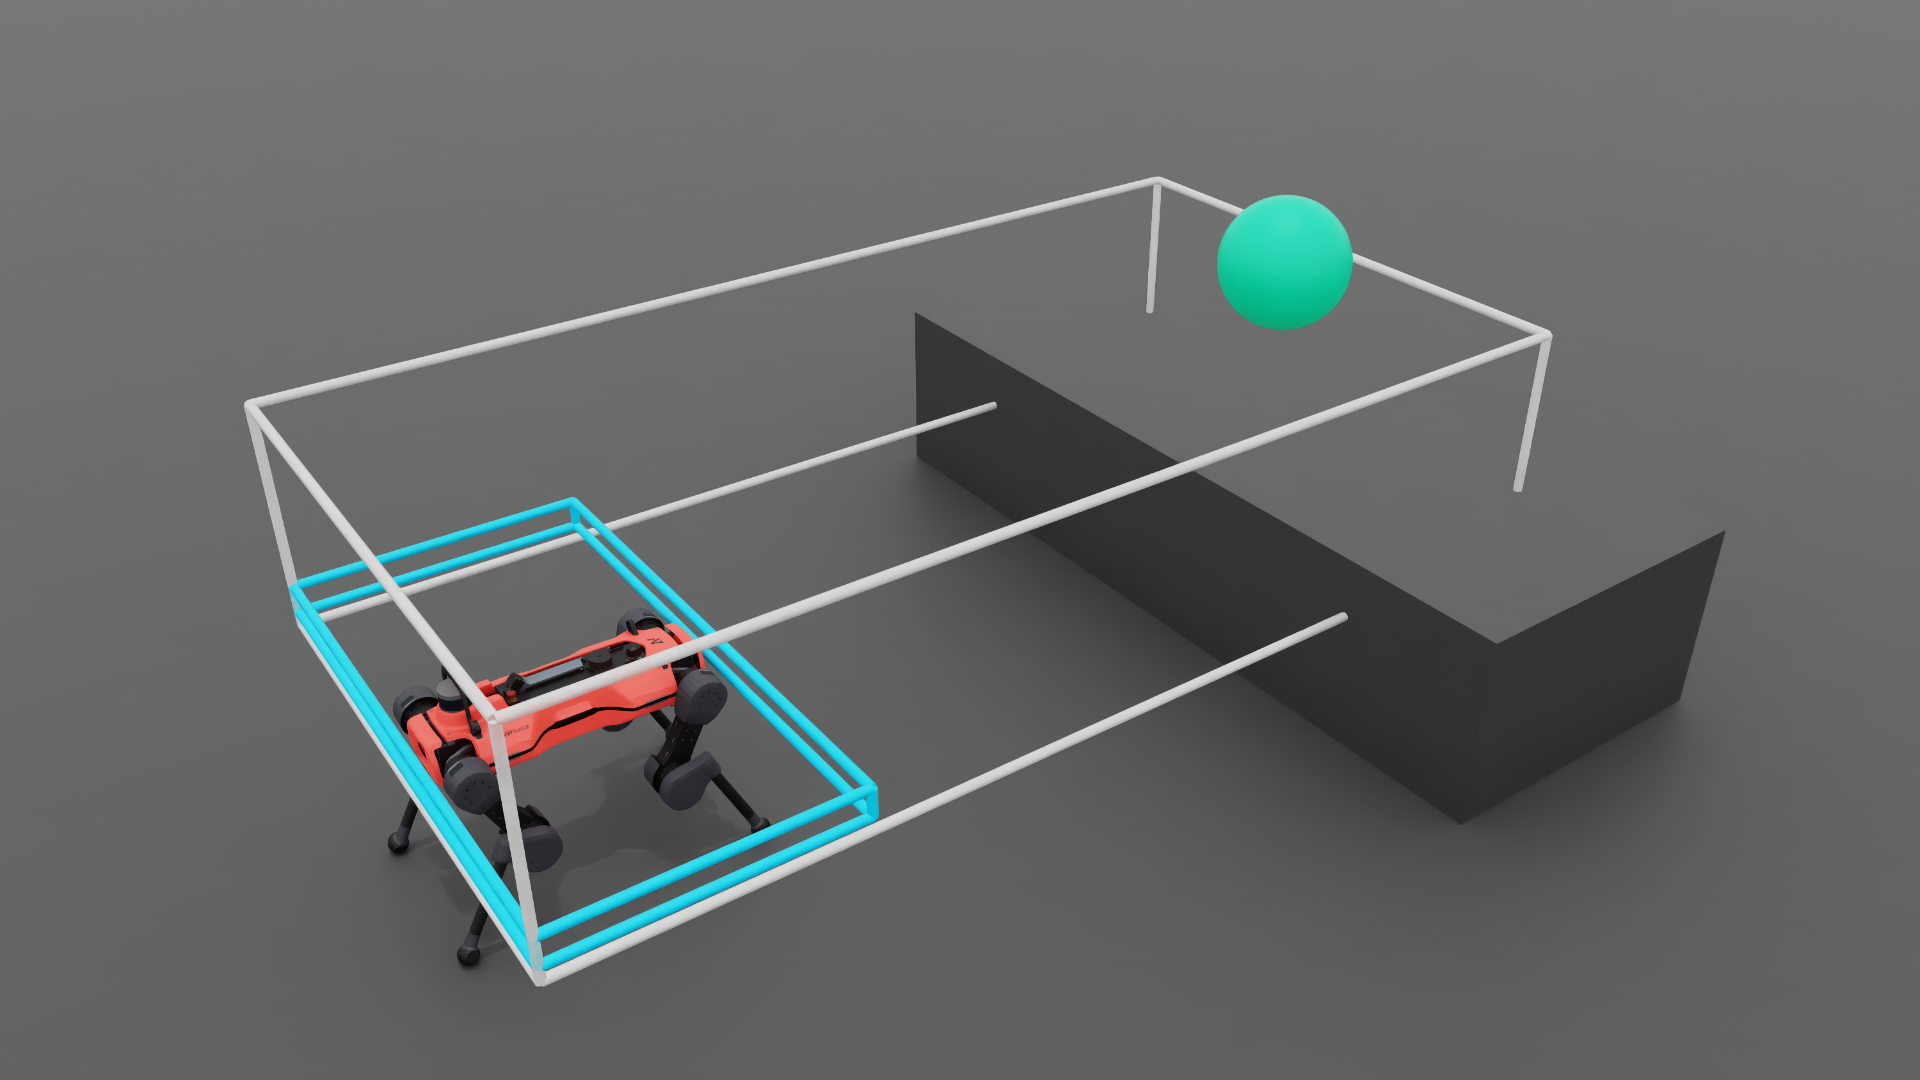
\includegraphics[width=\linewidth]{img/thumbnails/climb_box_up.png}
        \caption{Climb box up.}\label{fig:exp_renders_climb_box_up}
    \end{subfigure}
    \hfill
    \begin{subfigure}[t]{0.24\linewidth}
        \centering
        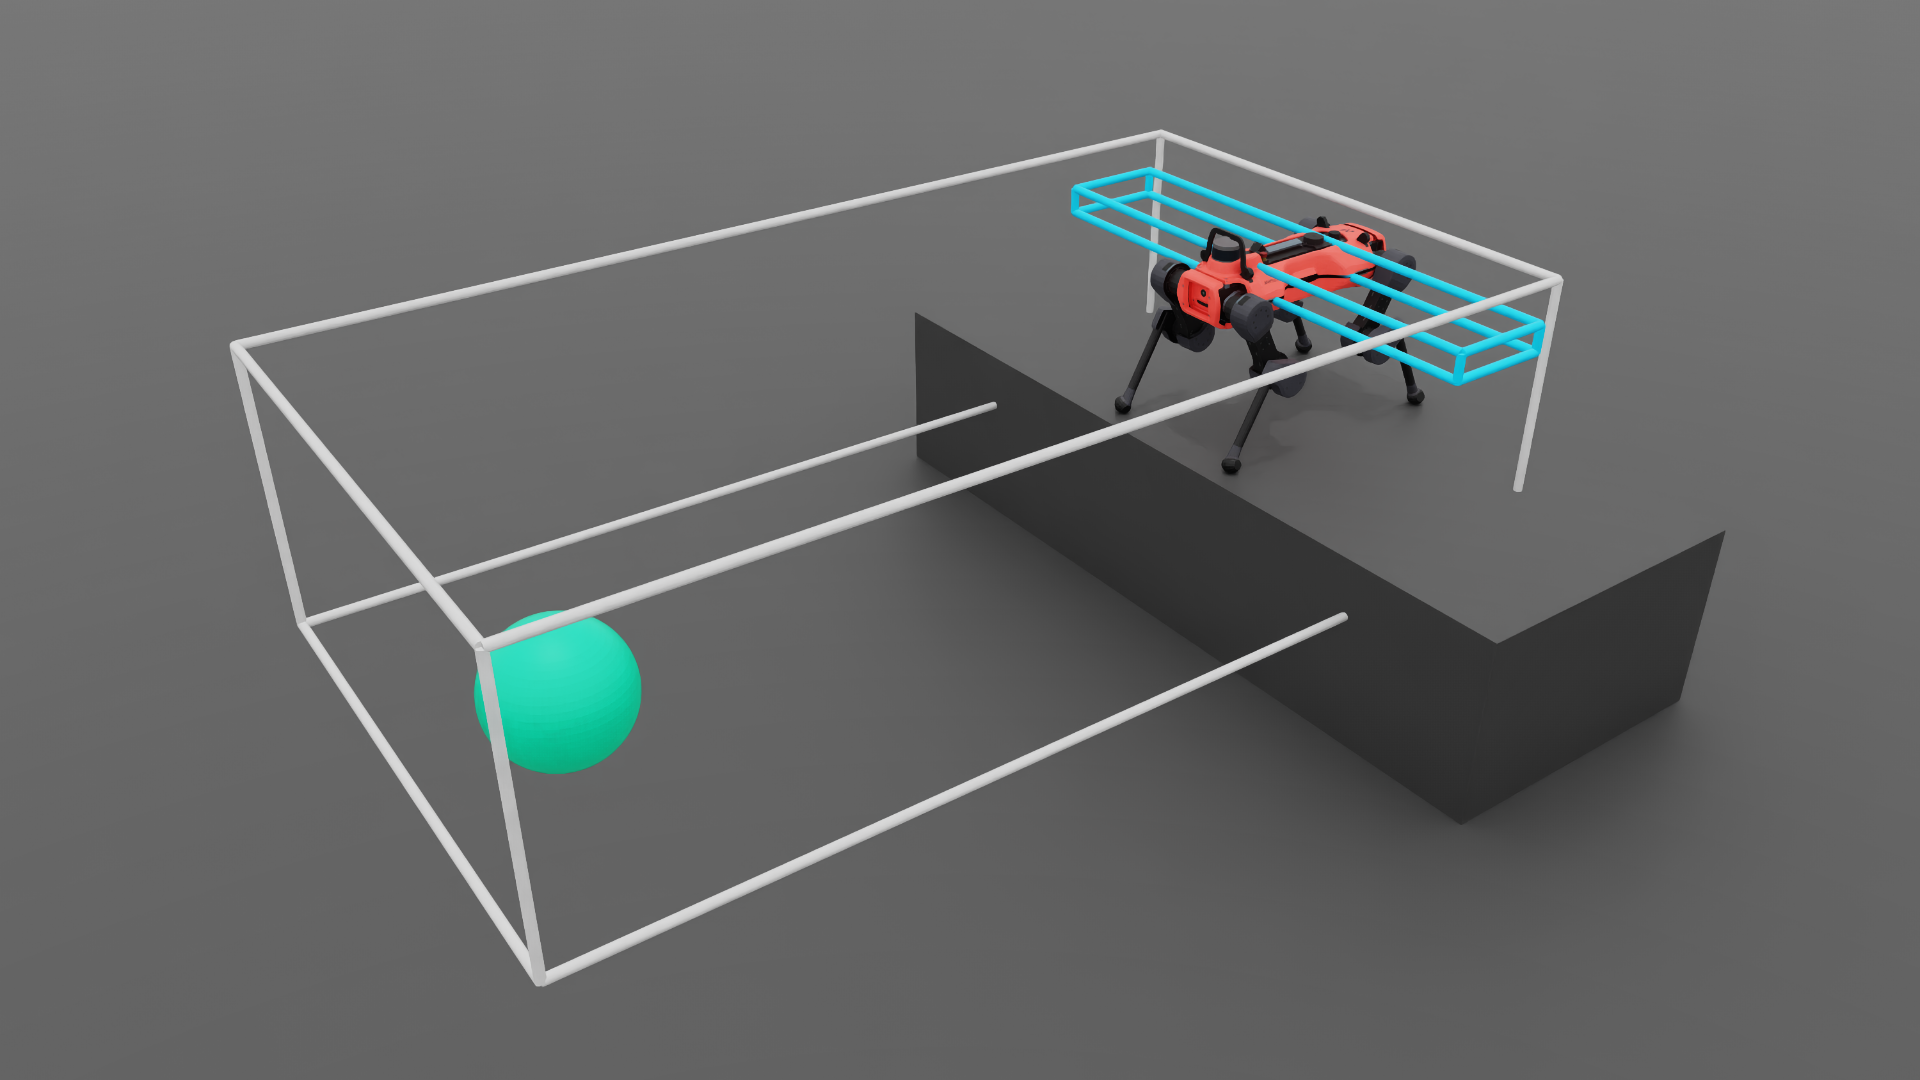
\includegraphics[width=\linewidth]{img/thumbnails/climb_box_down.png}
        \caption{Climb box down.}\label{fig:exp_renders_climb_box_down}
    \end{subfigure}
    \hfill
    \begin{subfigure}[t]{0.24\linewidth}
        \centering
        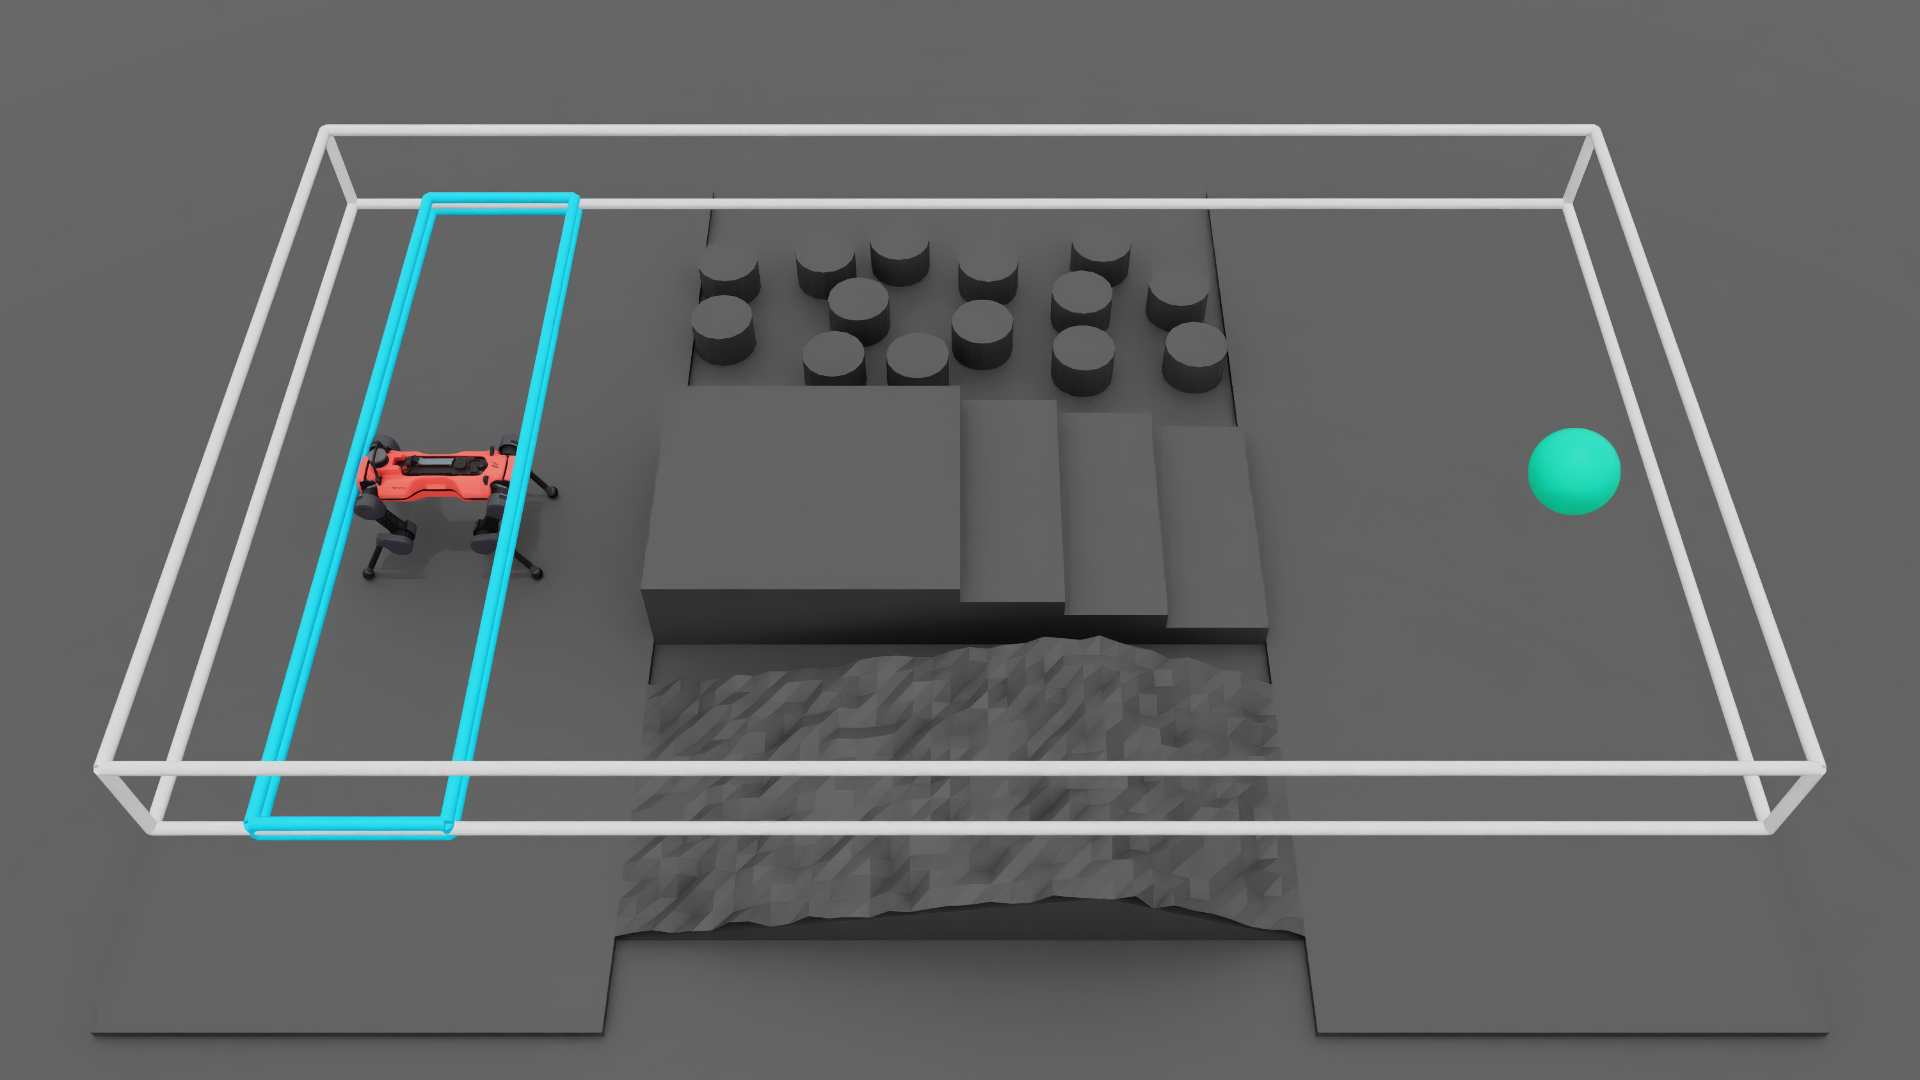
\includegraphics[width=\linewidth]{img/thumbnails/dtsg.png}
        \caption{Multiple terrain paths.}\label{fig:exp_renders_dtsg}
    \end{subfigure}
    \hfill
    \begin{subfigure}[t]{0.24\linewidth}
        \centering
        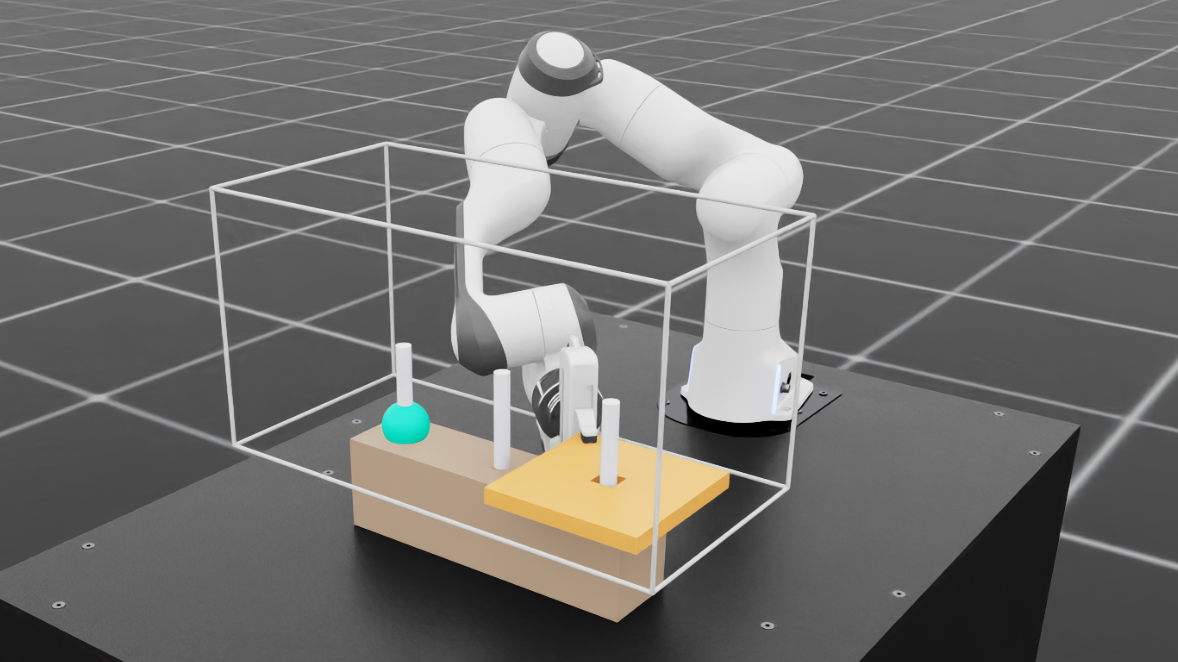
\includegraphics[width=\linewidth]{img/thumbnails/hanoi_p12.png}
        \caption{Tower of Hanoi.}\label{fig:exp_renders_hanoi_p12}
    \end{subfigure}
    \hfill\strut{}\\
    \hfill
    \begin{subfigure}[t]{0.24\linewidth}
        \centering
        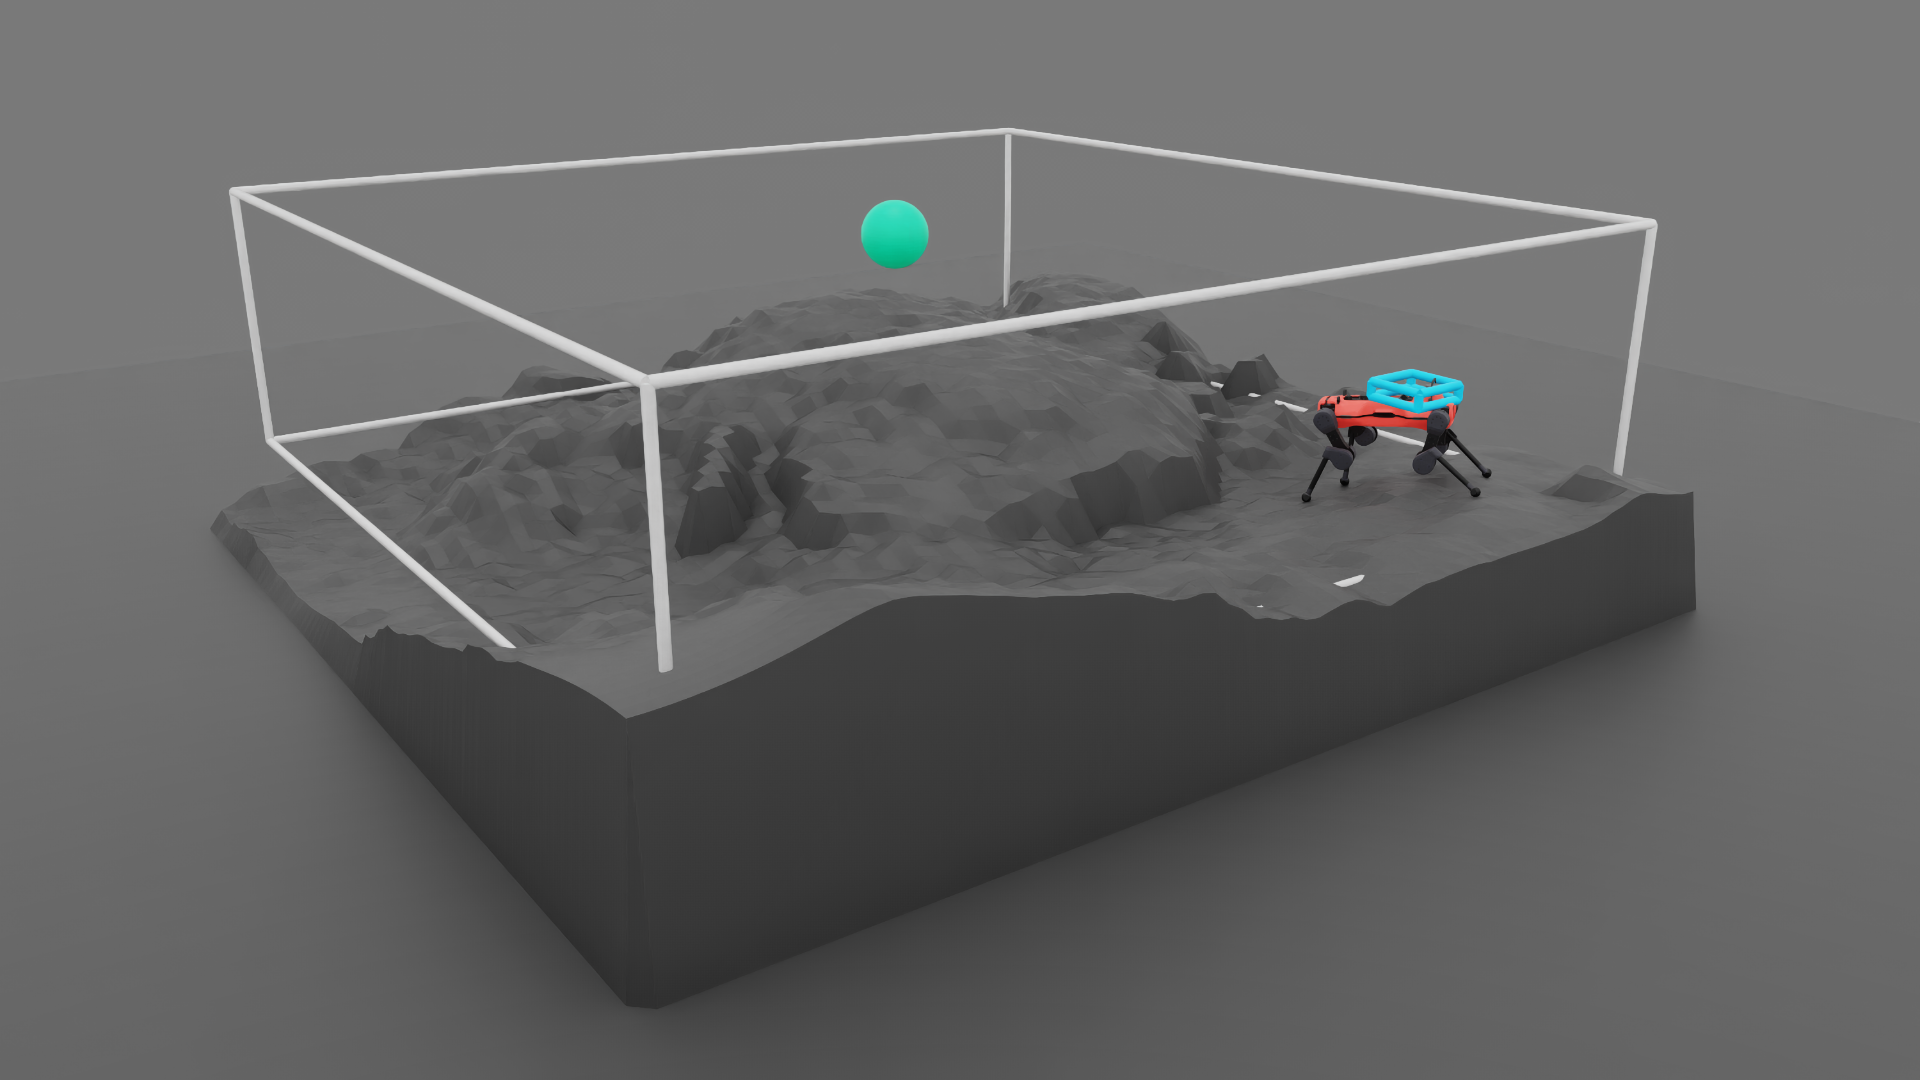
\includegraphics[width=\linewidth]{img/thumbnails/scan_boulder_small_rocks.png}
        \caption{Freestanding boulder I.}\label{fig:exp_renders_freestanding_boulder_I}
    \end{subfigure}
    \hfill
    \begin{subfigure}[t]{0.24\linewidth}
        \centering
        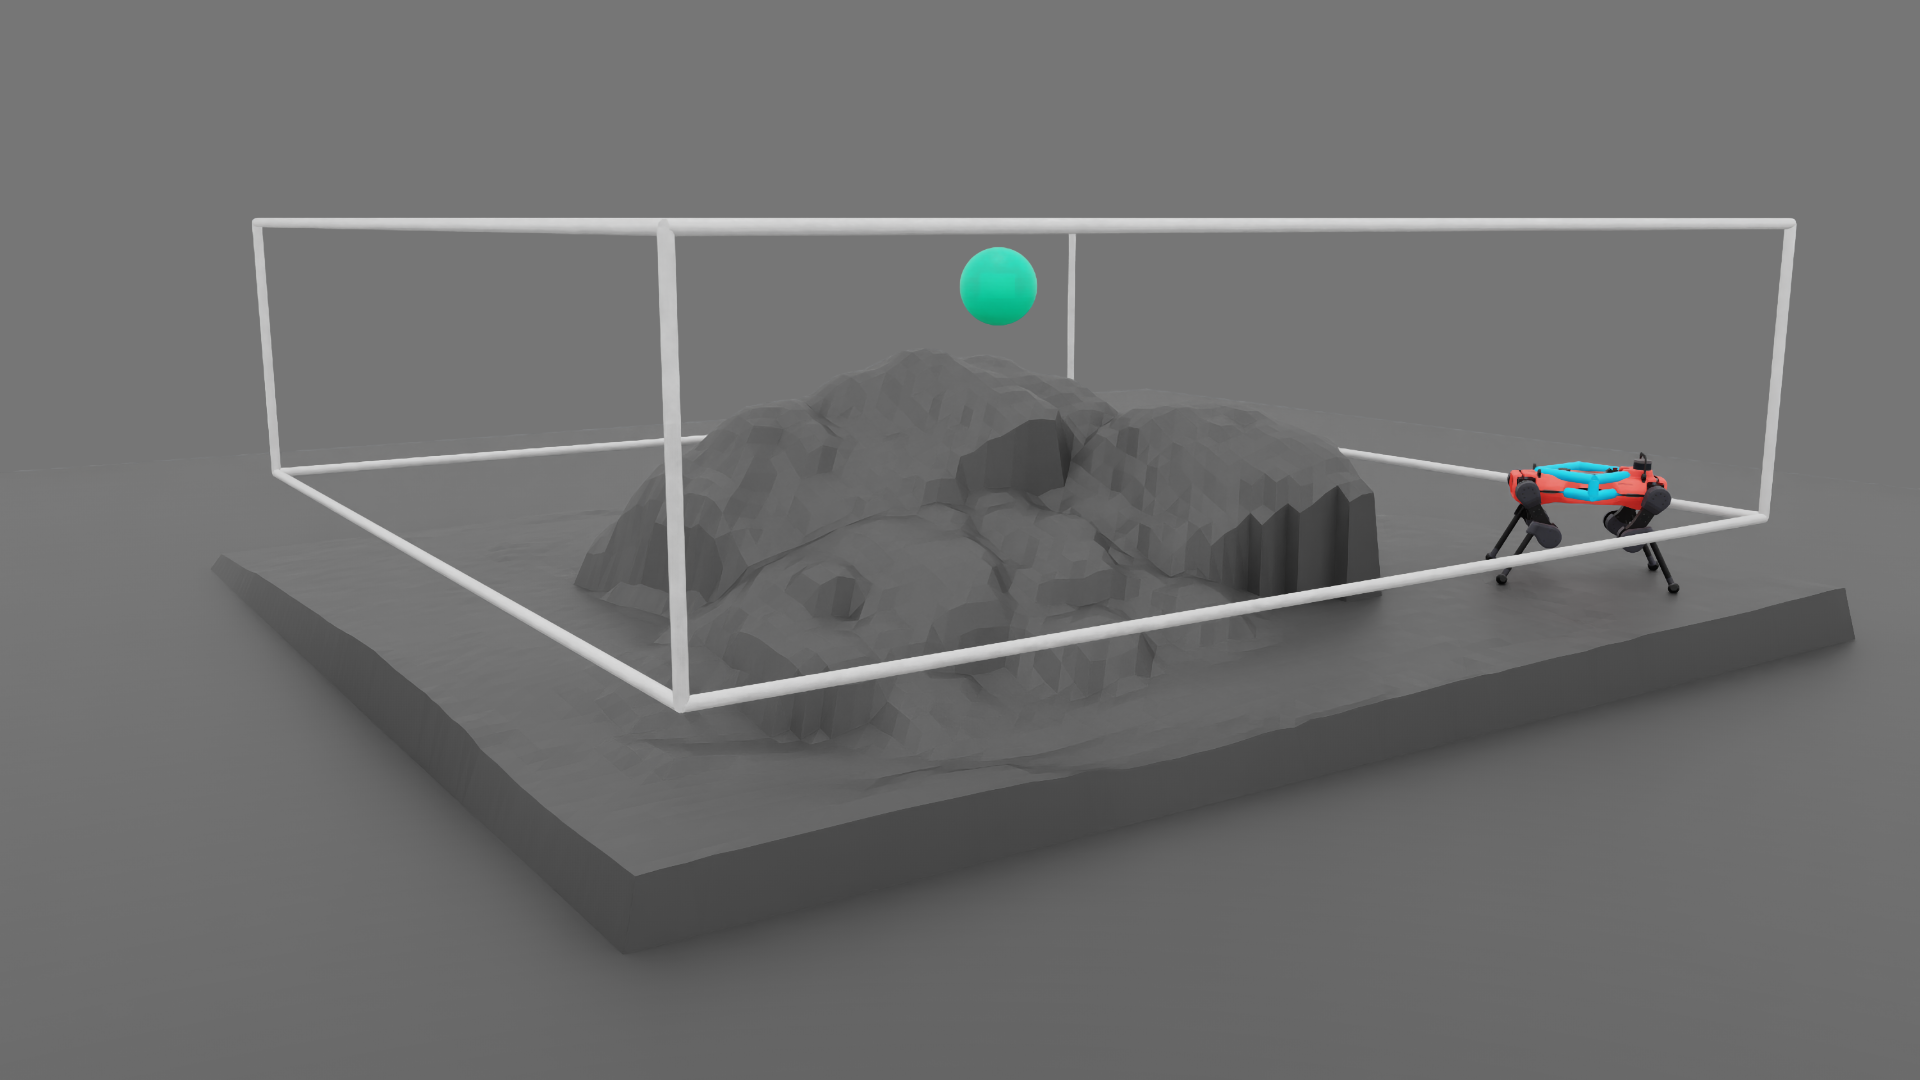
\includegraphics[width=\linewidth]{img/thumbnails/scan_freestanding_boulder.png}
        \caption{Freestanding boulder II.}\label{fig:exp_renders_freestanding_boulder_II}
    \end{subfigure}
    \hfill
    \begin{subfigure}[t]{0.24\linewidth}
        \centering
        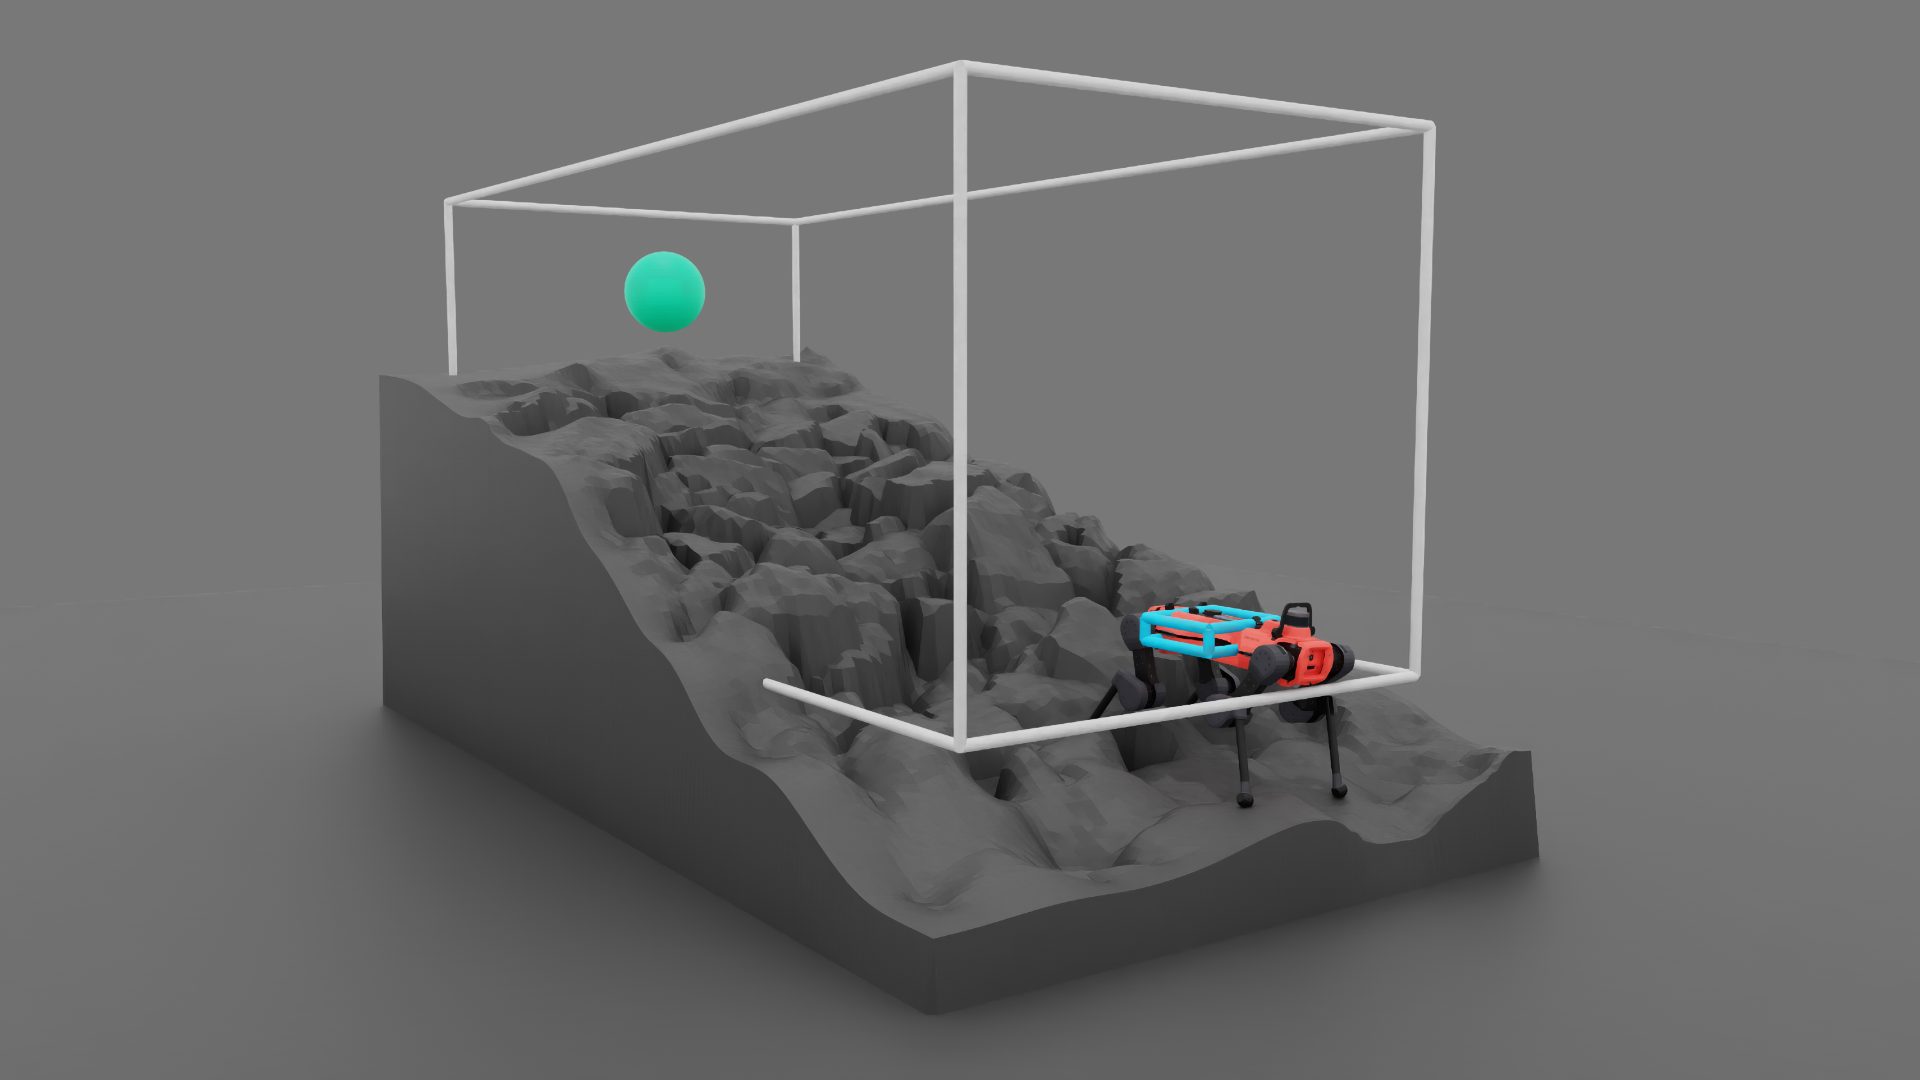
\includegraphics[width=\linewidth]{img/thumbnails/scan_rocky_ascent.png}
        \caption{Rocky ascent.}\label{fig:exp_renders_rocky_ascent}
    \end{subfigure}
    \hfill
    \begin{subfigure}[t]{0.24\linewidth}
        \centering
        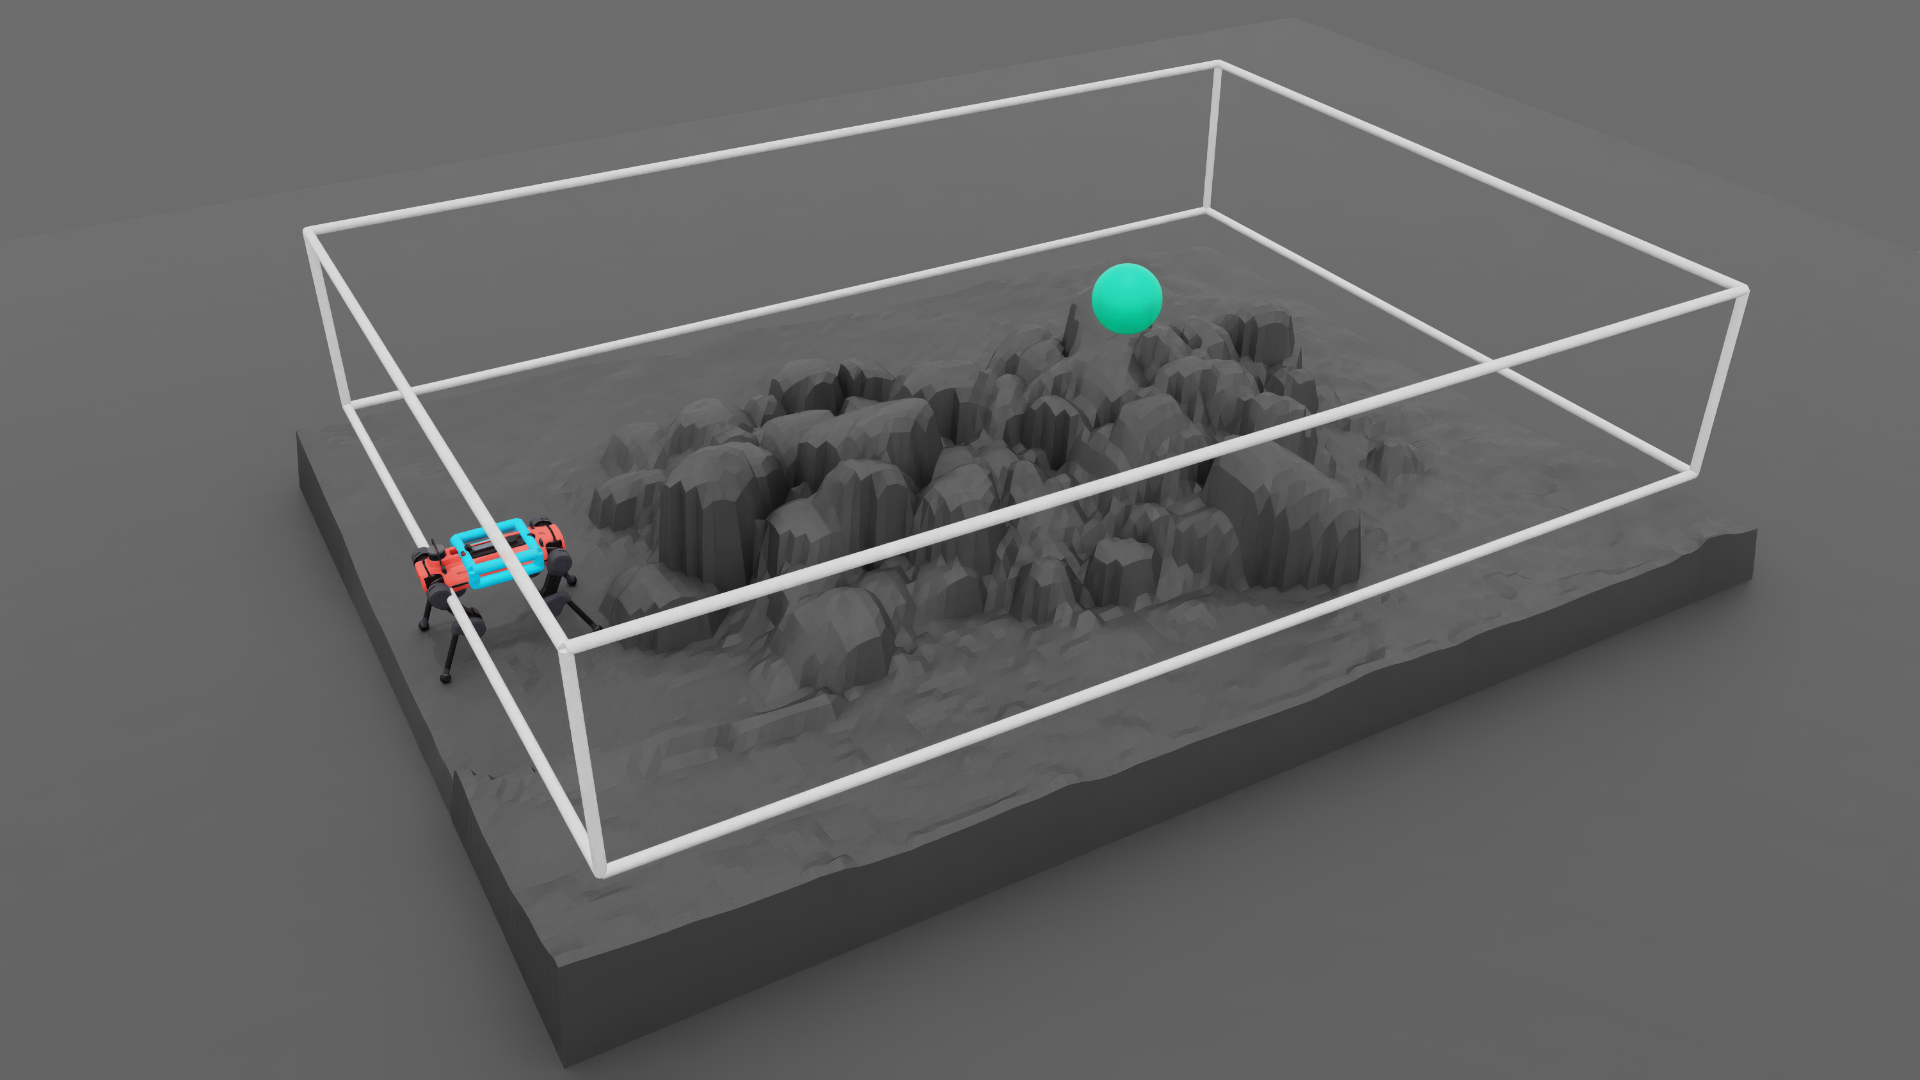
\includegraphics[width=\linewidth]{img/thumbnails/scan_small_rocks.png}
        \caption{Small stone field.}\label{fig:exp_renders_small_rocks}
    \end{subfigure}
    \hfill
    \caption{Experimental setup. {\color{cyan}Cyan} indicates the initial distribution, {\color{teal} green} the target goal, and the white box represents the task space.}\label{fig:experiment_renders}
\end{figure}

In all experiments, the rewards are defined as a combination of the sparse goal reward from Section~\ref{sec:problem_formulation} with $\epsilon = 0.25\,\mathrm{m}$, i.e., the agent has to reach the goal within a certain distance, and a termination penalty for collisions of the base with the terrain.

In the \textit{multiple terrain paths} experiments, a potential-based reward shaping term~\citep{ng1999policy}, which leaves the set of optimal policies of the underlying GA-MDP unchanged, is added to provide a reward signal strong enough for the no-curriculum PPO baseline to find solutions:
\begin{equation*}
    r_{\mathrm{progress}}(s_t, s_{t+1}, g) = \lVert \phi(s_t) - g \rVert - \gamma \lVert \phi(s_{t+1}) - g \rVert
\end{equation*}

\subsection{Sample Efficiency and Robustness}\label{sec:exp_main}
To evaluate sample efficiency and robustness, we compare our method BVER against state-of-the-art curriculum learning methods on a sparse-reward box climbing task. The task is defined as a goal-conditioned locomotion task where the agent has to reach a target goal position on top of a box from an initial distribution of start positions in front of the box. The task is challenging due to the sparse reward signal and the long horizon required to reach the goal.
\paragraph{Sample Efficiency:}
The results in Figure~\ref{fig:bench} already show a clear distinction between the vanilla PPO baseline, the curricula and the imitation learning methods (marked with $\star$). The policies trained on the initial distributions and no curriculum (vanilla PPO) are unable to solve the task, while training with random starts achieves a success rate of more than 95\%. This shows that the reward signal is attainable and the task solvable by initializing the agent closer to the goal.
Backplay~\citep{resnick2018backplay} shows the fastest convergence, and its advantage over RSI~\citep{peng2018deepmimic} shows the importance of ordering the task over training time. For the reference-free curricula, our method BVER shows the fastest convergence and highest success rate, outperforming both RC~\citep{florensa2017reverse} and random starts, while even surpassing RSI. BVER reaches a success rate of 95\% in roughly 65\% fewer training iterations than the best reference-free baseline.
% TODO: verify the 65% against the logged iteration counts (mean over seeds) and name the baseline.

\paragraph{Robustness:}
We evaluate the trained policies on (1) perturbations to the yaw angle used in the initialization, (2) variations in start positions (goal set to the target goal), and (3) variations in goal positions (initialized on the initial distribution). The results in Figure~\ref{fig:robustness} show that BVER's bidirectional curriculum leads to policies that can solve the task under various start-goal configurations, while the other curricula fail to generalize to unseen configurations.
\begin{figure}[h]
    \centering
    \hfill
    \begin{subfigure}[c]{0.6\linewidth}
        \centering
        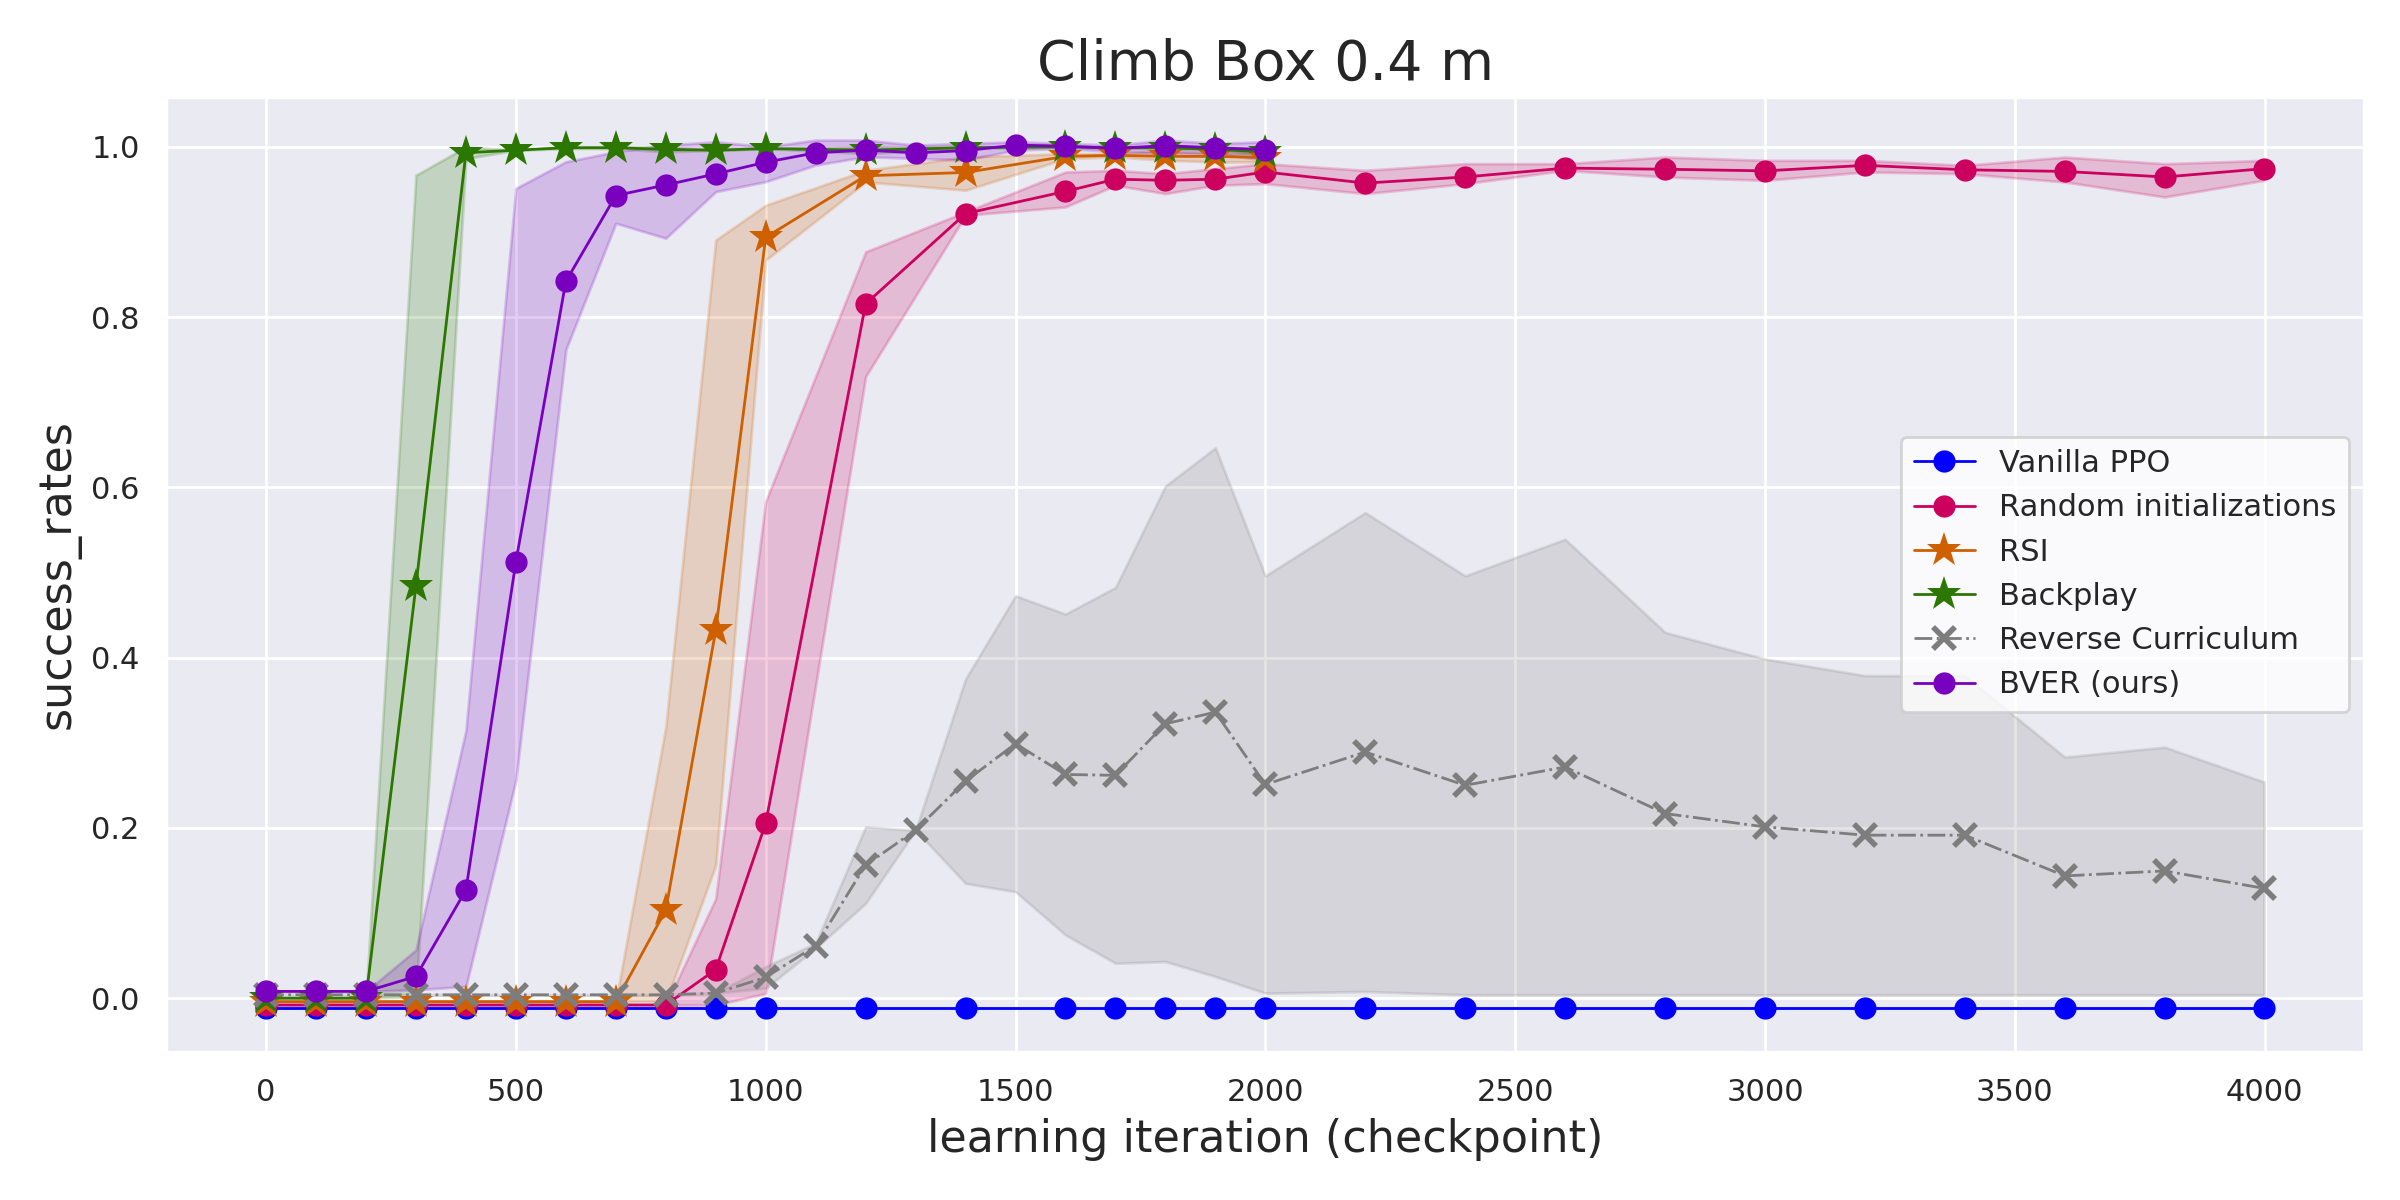
\includegraphics[width=\linewidth]{img/sb/eval_comparison_41_up_clean_comp.png}
        \caption{BVER is able to achieve a success rate of over 95\% faster than all other reference-free curricula and even faster than one reference-based method (RSI).}\label{fig:bench}
    \end{subfigure}
    \hfill
    \begin{subfigure}[c]{0.3\linewidth}
        \centering
        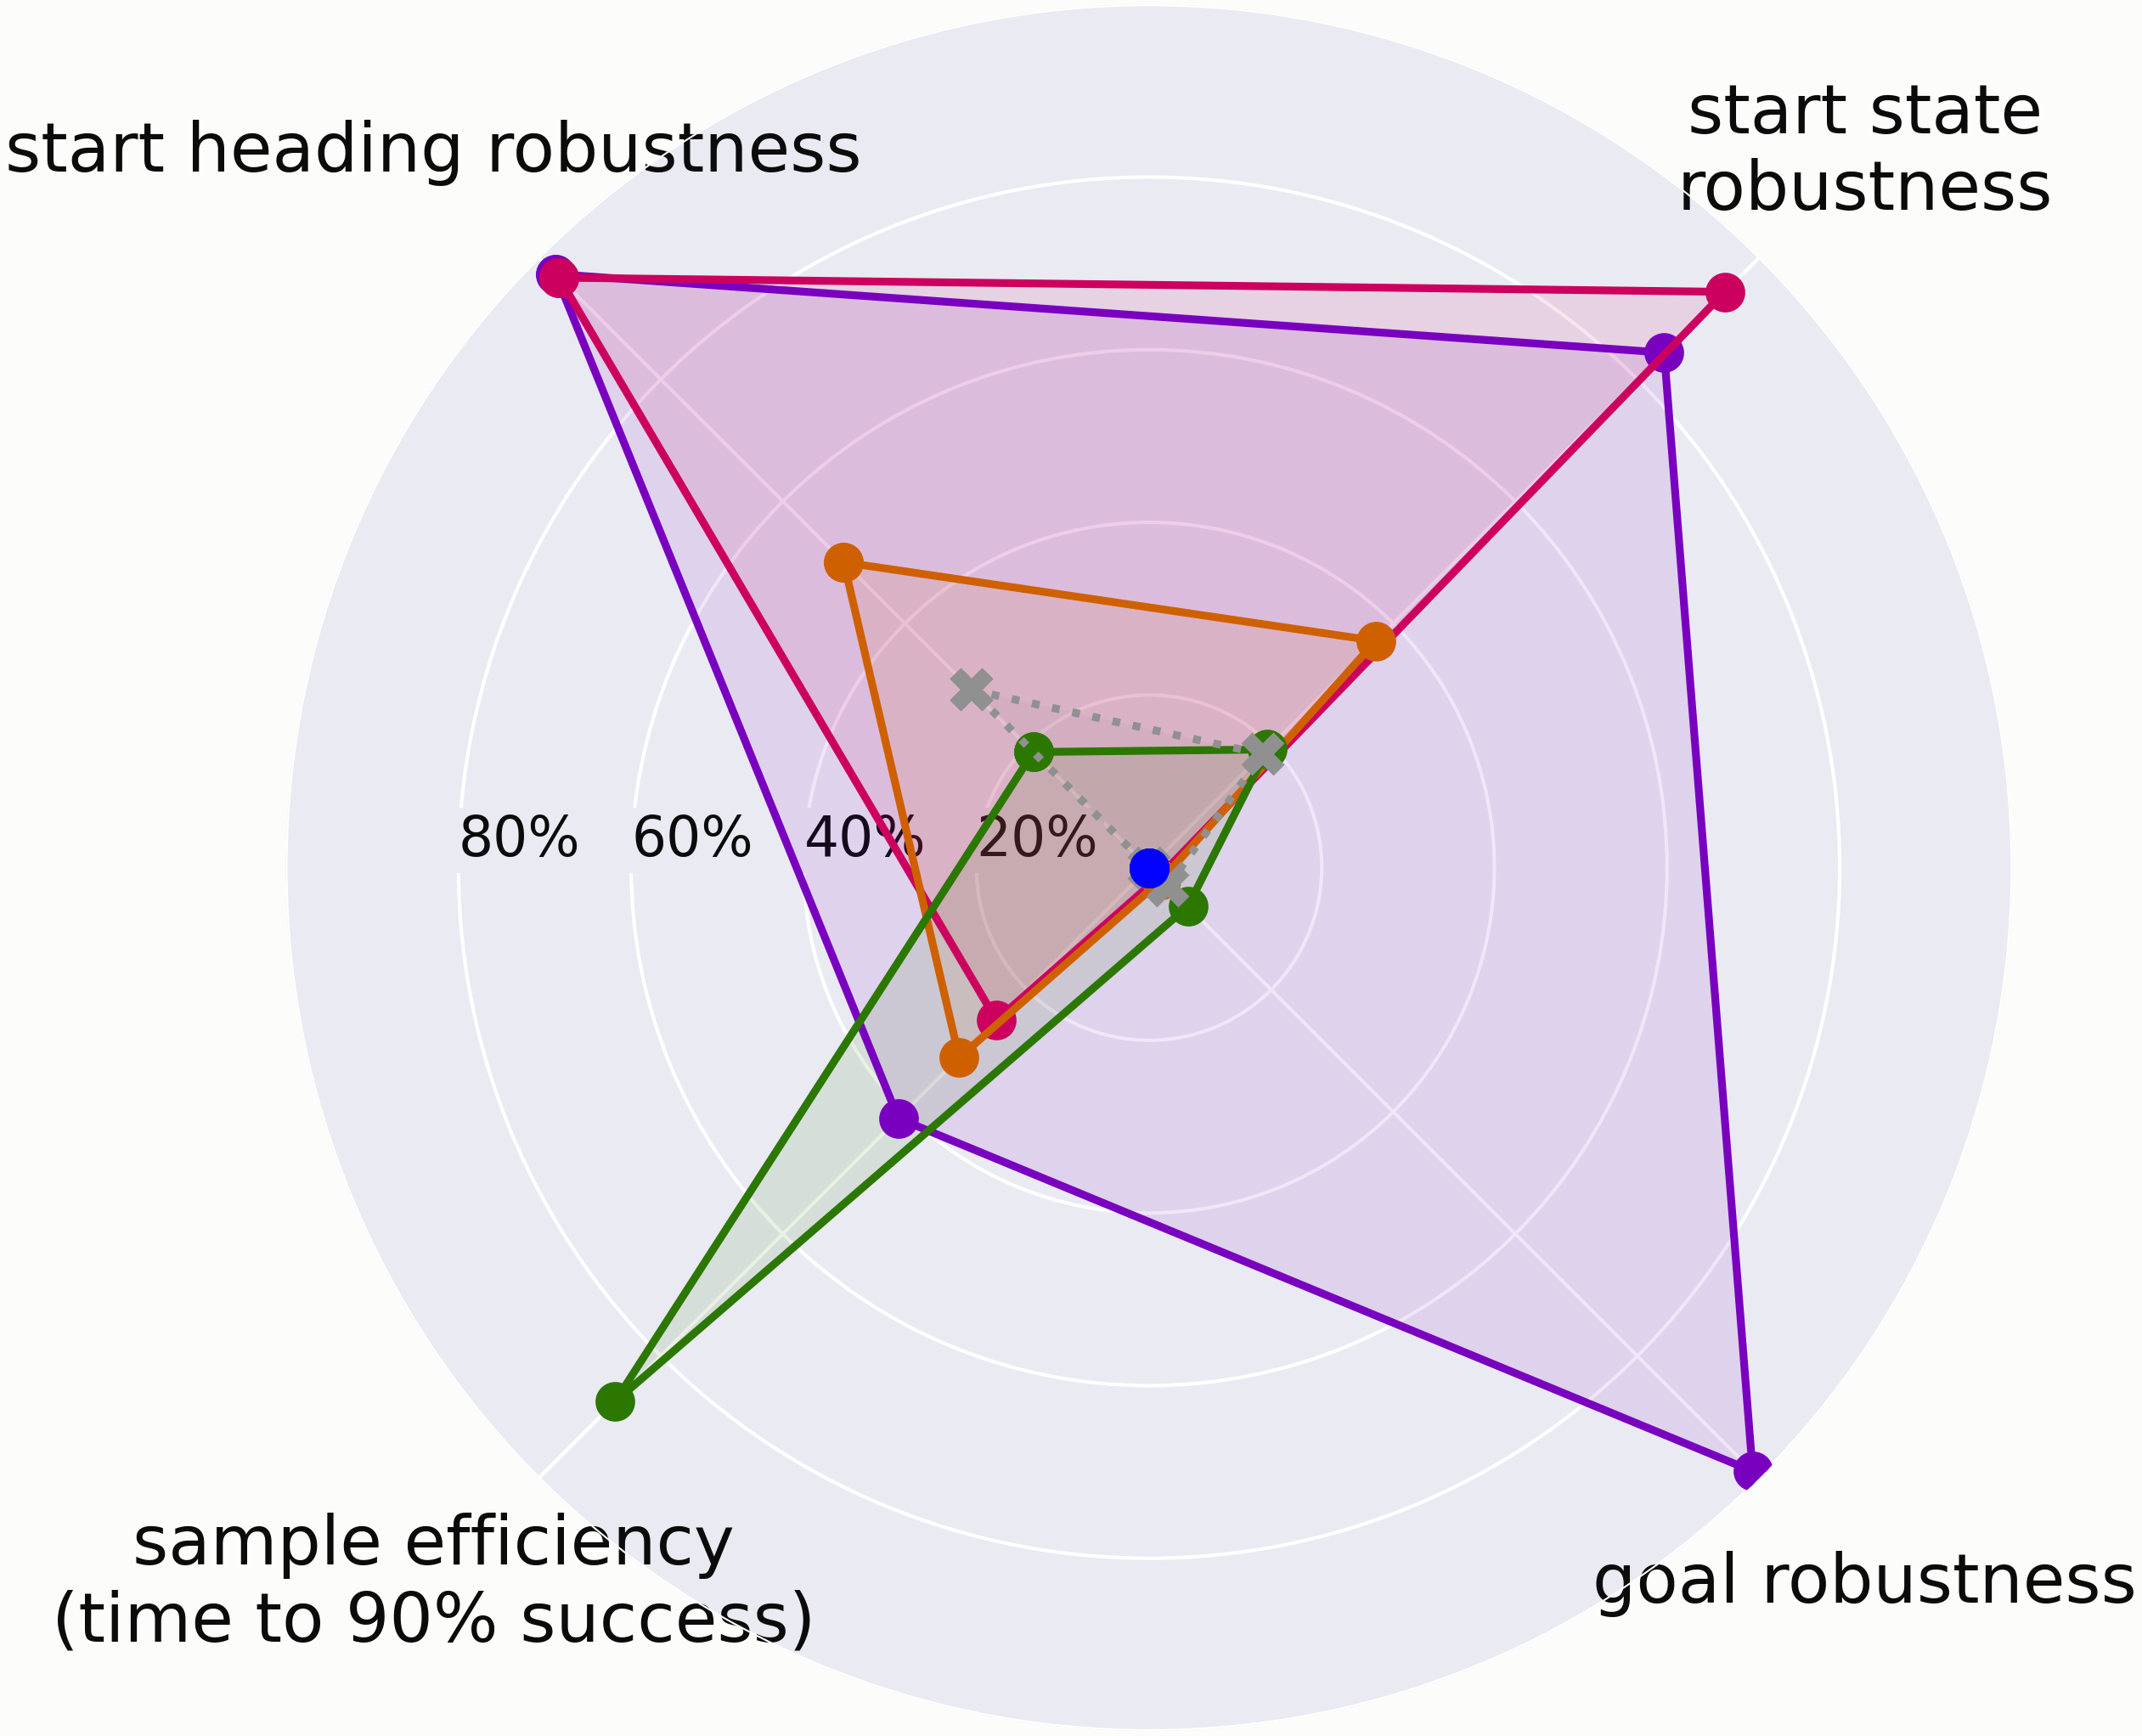
\includegraphics[width=\linewidth]{img/sb/robustness_spider_headline_nolegend.png}
        \caption{BVER's start-goal curriculum leads to policies that can solve the task under various start-goal configurations.}\label{fig:robustness}
    \end{subfigure}
    \hfill\strut{}
    \caption{Sample efficiency and robustness evaluated on a sparse-reward box climbing task.}\label{fig:eval_04}
\end{figure}

\subsection{Ablations: Forwards / Backwards Symmetry}\label{sec:exp_ablations}

\paragraph{Maze ablations:}\label{sec:exp_ablations_maze}
To evaluate the contribution of individual components of BVER, we conduct further ablation studies on three maze environments (Figure~\ref{fig:maze_layout}) similar to those used in prior work~\citep{florensa2017reverse,cho2023outcome}. Specifically, the agent ({\color{orange}orange point mass}) has to find a path from the initial distribution ({\color{cyan}cyan rectangle}) to the goal ({\color{teal}green ball}). First, we evaluate the effect of our curriculum against a baseline that does not use any curriculum (\textit{vanilla PPO}) and a simple curriculum that samples intermediate goals (to reach from the start) and intermediate starts (from which to reach the target goal) randomly from the free space (\textit{random initializations}). The results in Figure~\ref{fig:maze_ablation_bench} show that both curricula enable finding solutions in all three environments, whereas vanilla PPO does not. In the more complex \textit{N-maze} and \textit{large-maze} environments, BVER shows faster convergence than the random curriculum.

We compare using only the forwards expansion, only the backwards expansion, and the bidirectional expansion in Figure~\ref{fig:maze_ablation_dir}. In addition, we evaluate the effect of connecting the two frontiers by comparing a version of BVER that only samples from the task space to a version that samples from both the task space and the other frontier. The results in Figure~\ref{fig:maze_ablation_connect} show that connecting the two frontiers leads to better sample efficiency in the cases where the optimal path covers only a small fraction of the total search space (\textit{N-maze} and \textit{large-maze}). However, there is no significant difference between connect ratios above 0.5.
\begin{figure}[h]
    \centering
    \hfill
    \begin{subfigure}[c]{0.11\linewidth}
        \centering
        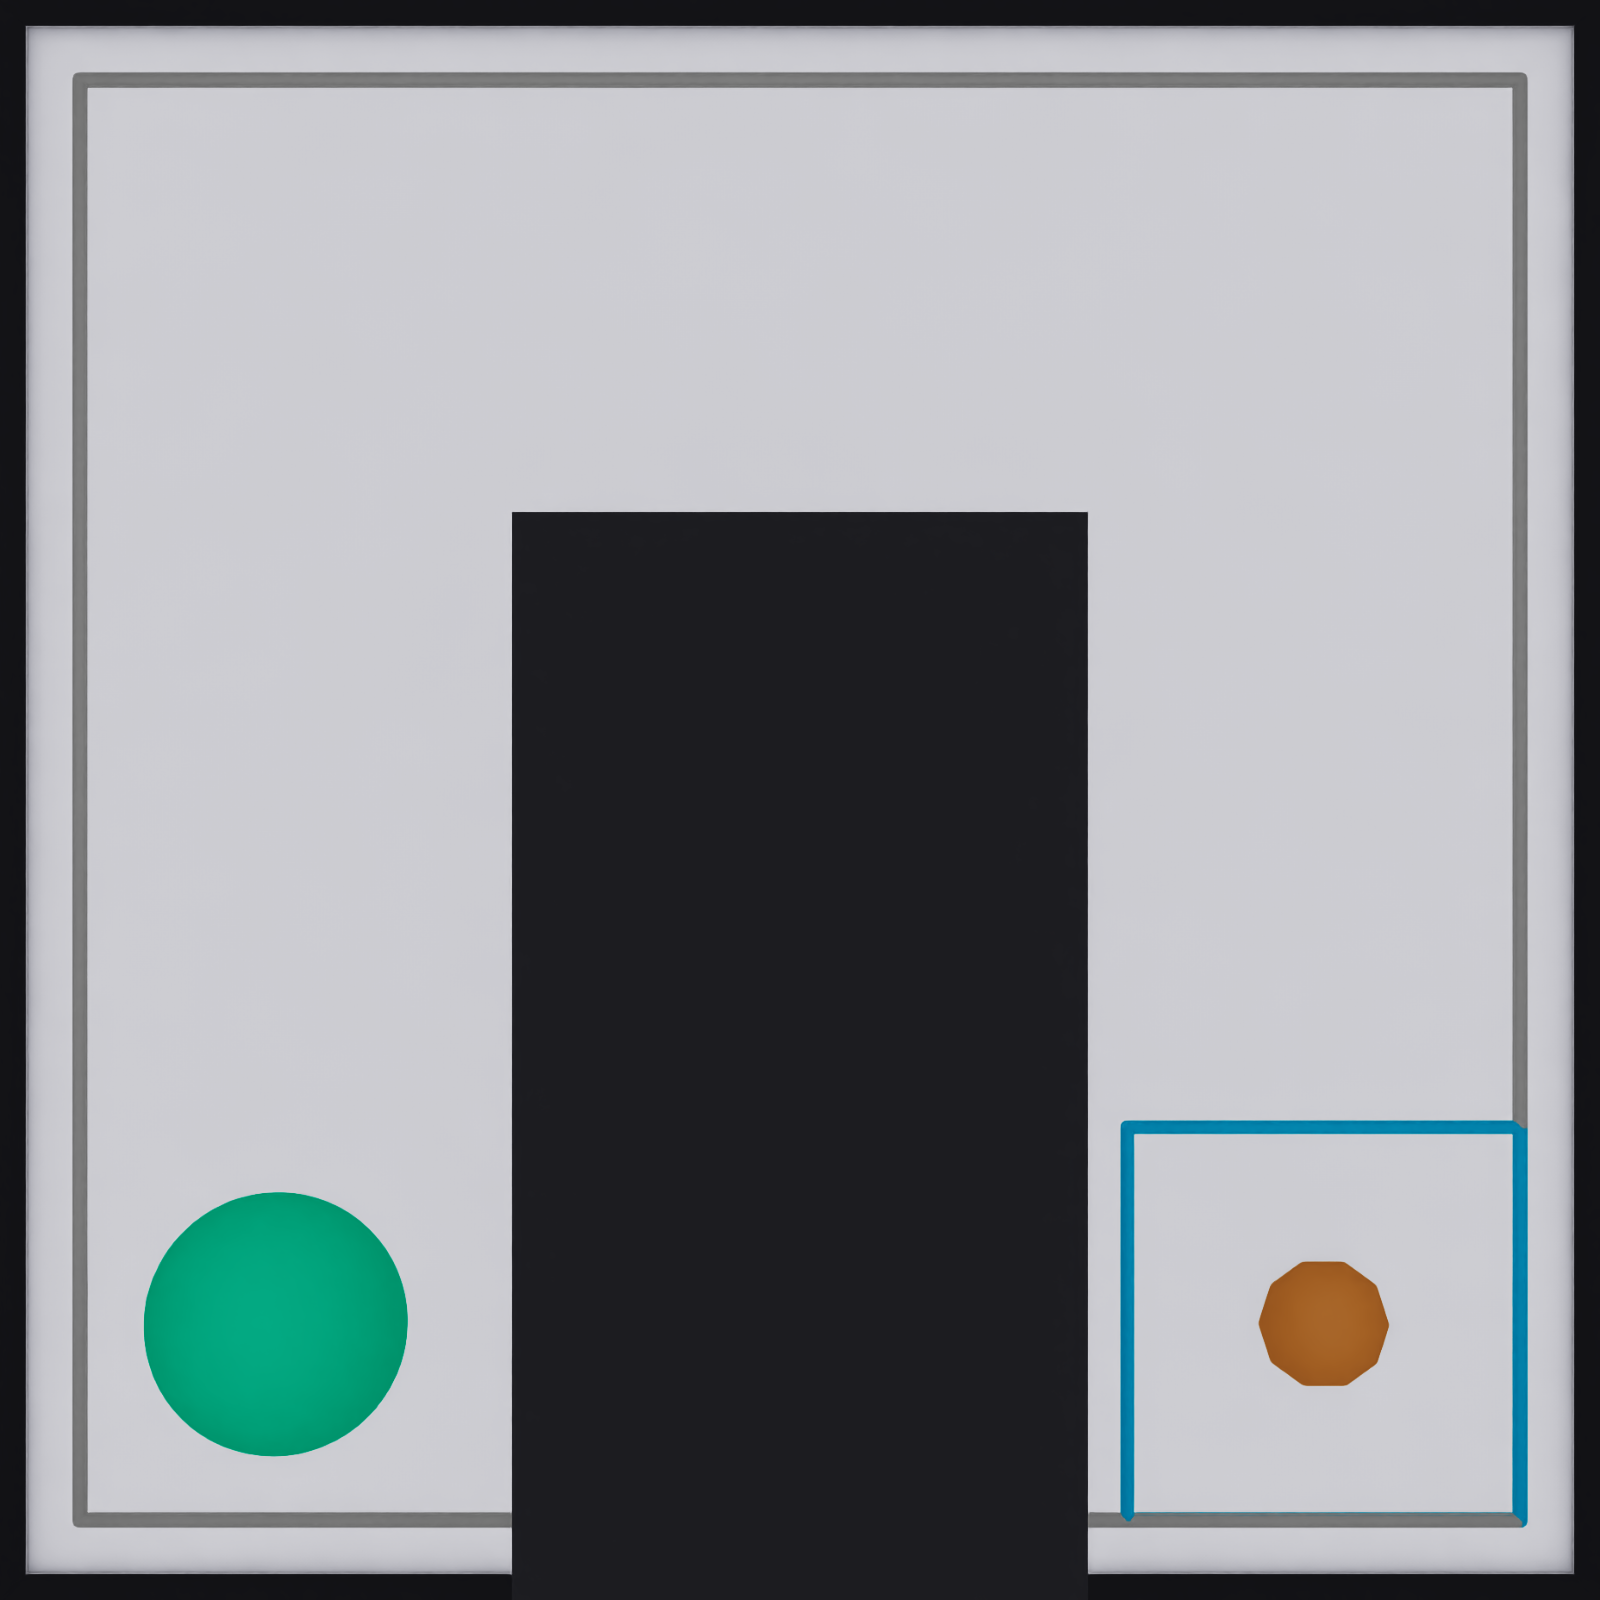
\includegraphics[width=\linewidth]{img/maze/layouts/maze_u.png}
    \end{subfigure}
    \hfill
    \begin{subfigure}[c]{0.29\linewidth}
        \centering
        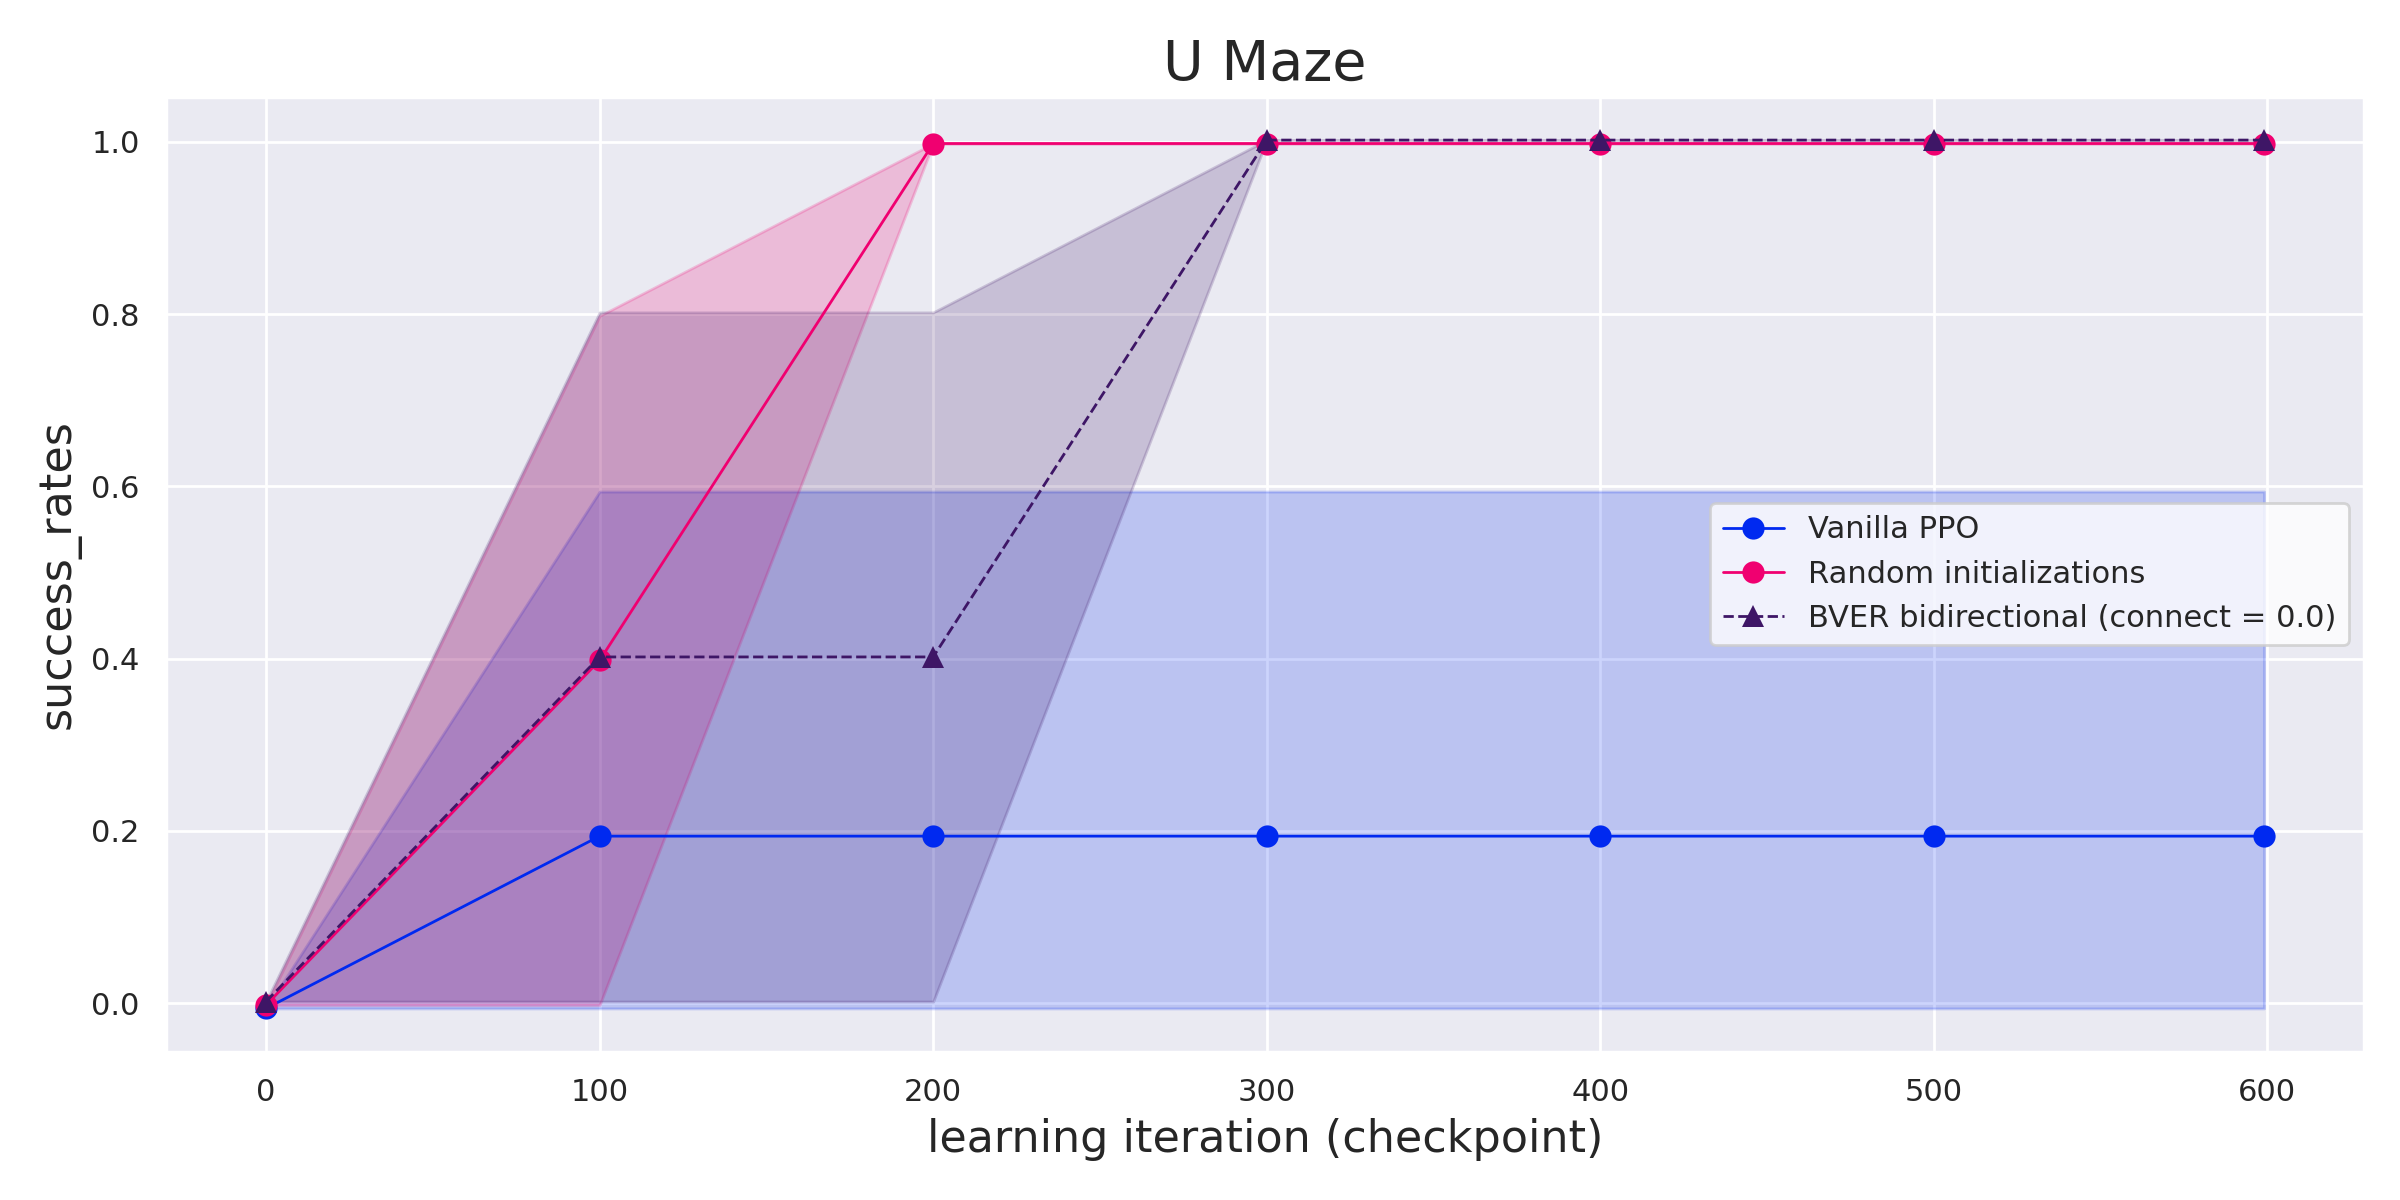
\includegraphics[width=\linewidth]{img/maze/u/eval_comparison_u_maze_bench.png}
    \end{subfigure}
    \hfill
    \begin{subfigure}[c]{0.29\linewidth}
        \centering
        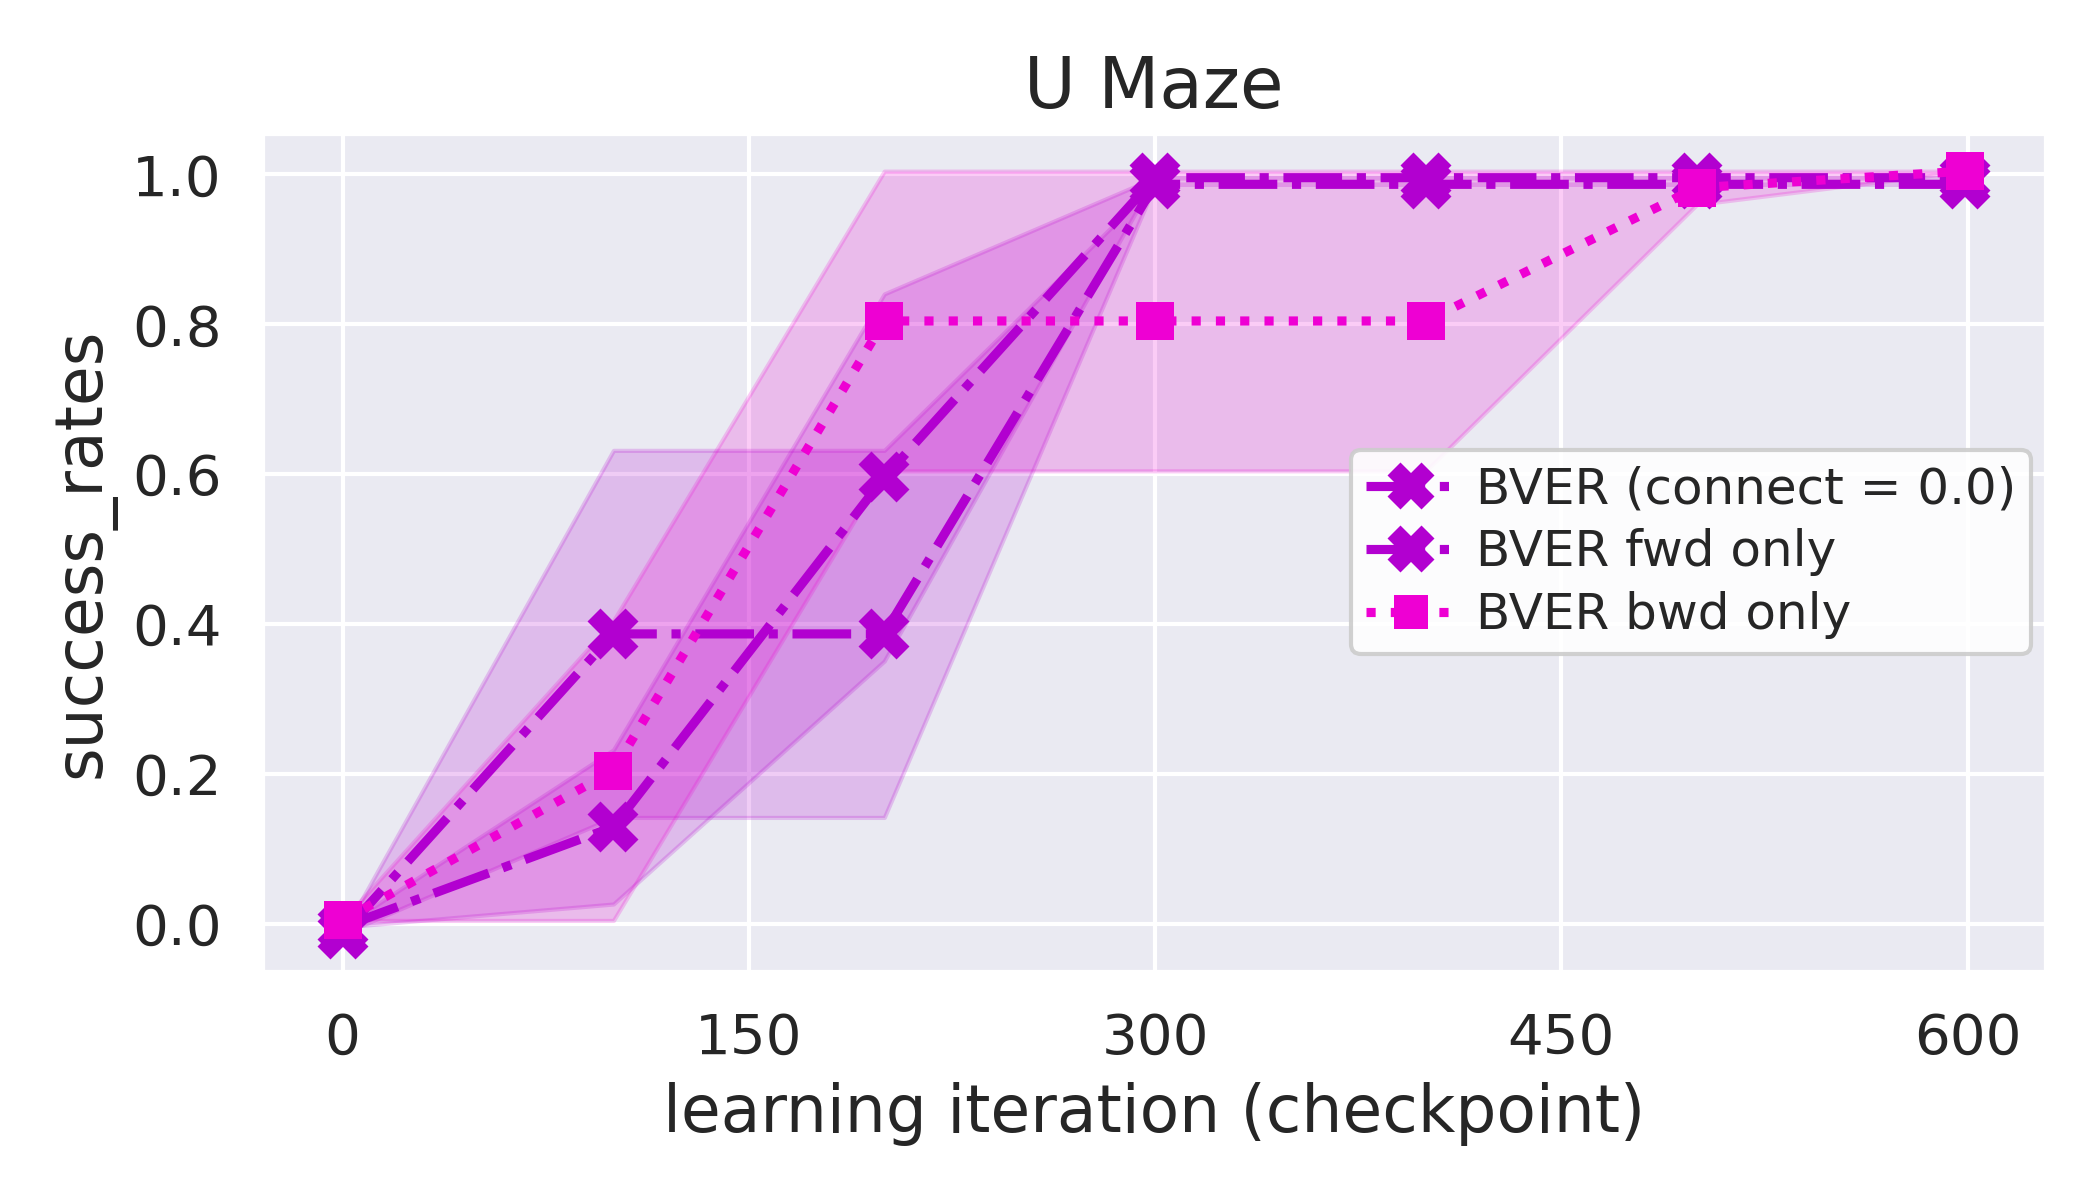
\includegraphics[width=\linewidth]{img/maze/u/eval_comparison_u_maze_abl_dir.png}
    \end{subfigure}
    \hfill
    \begin{subfigure}[c]{0.29\linewidth}
        \centering
        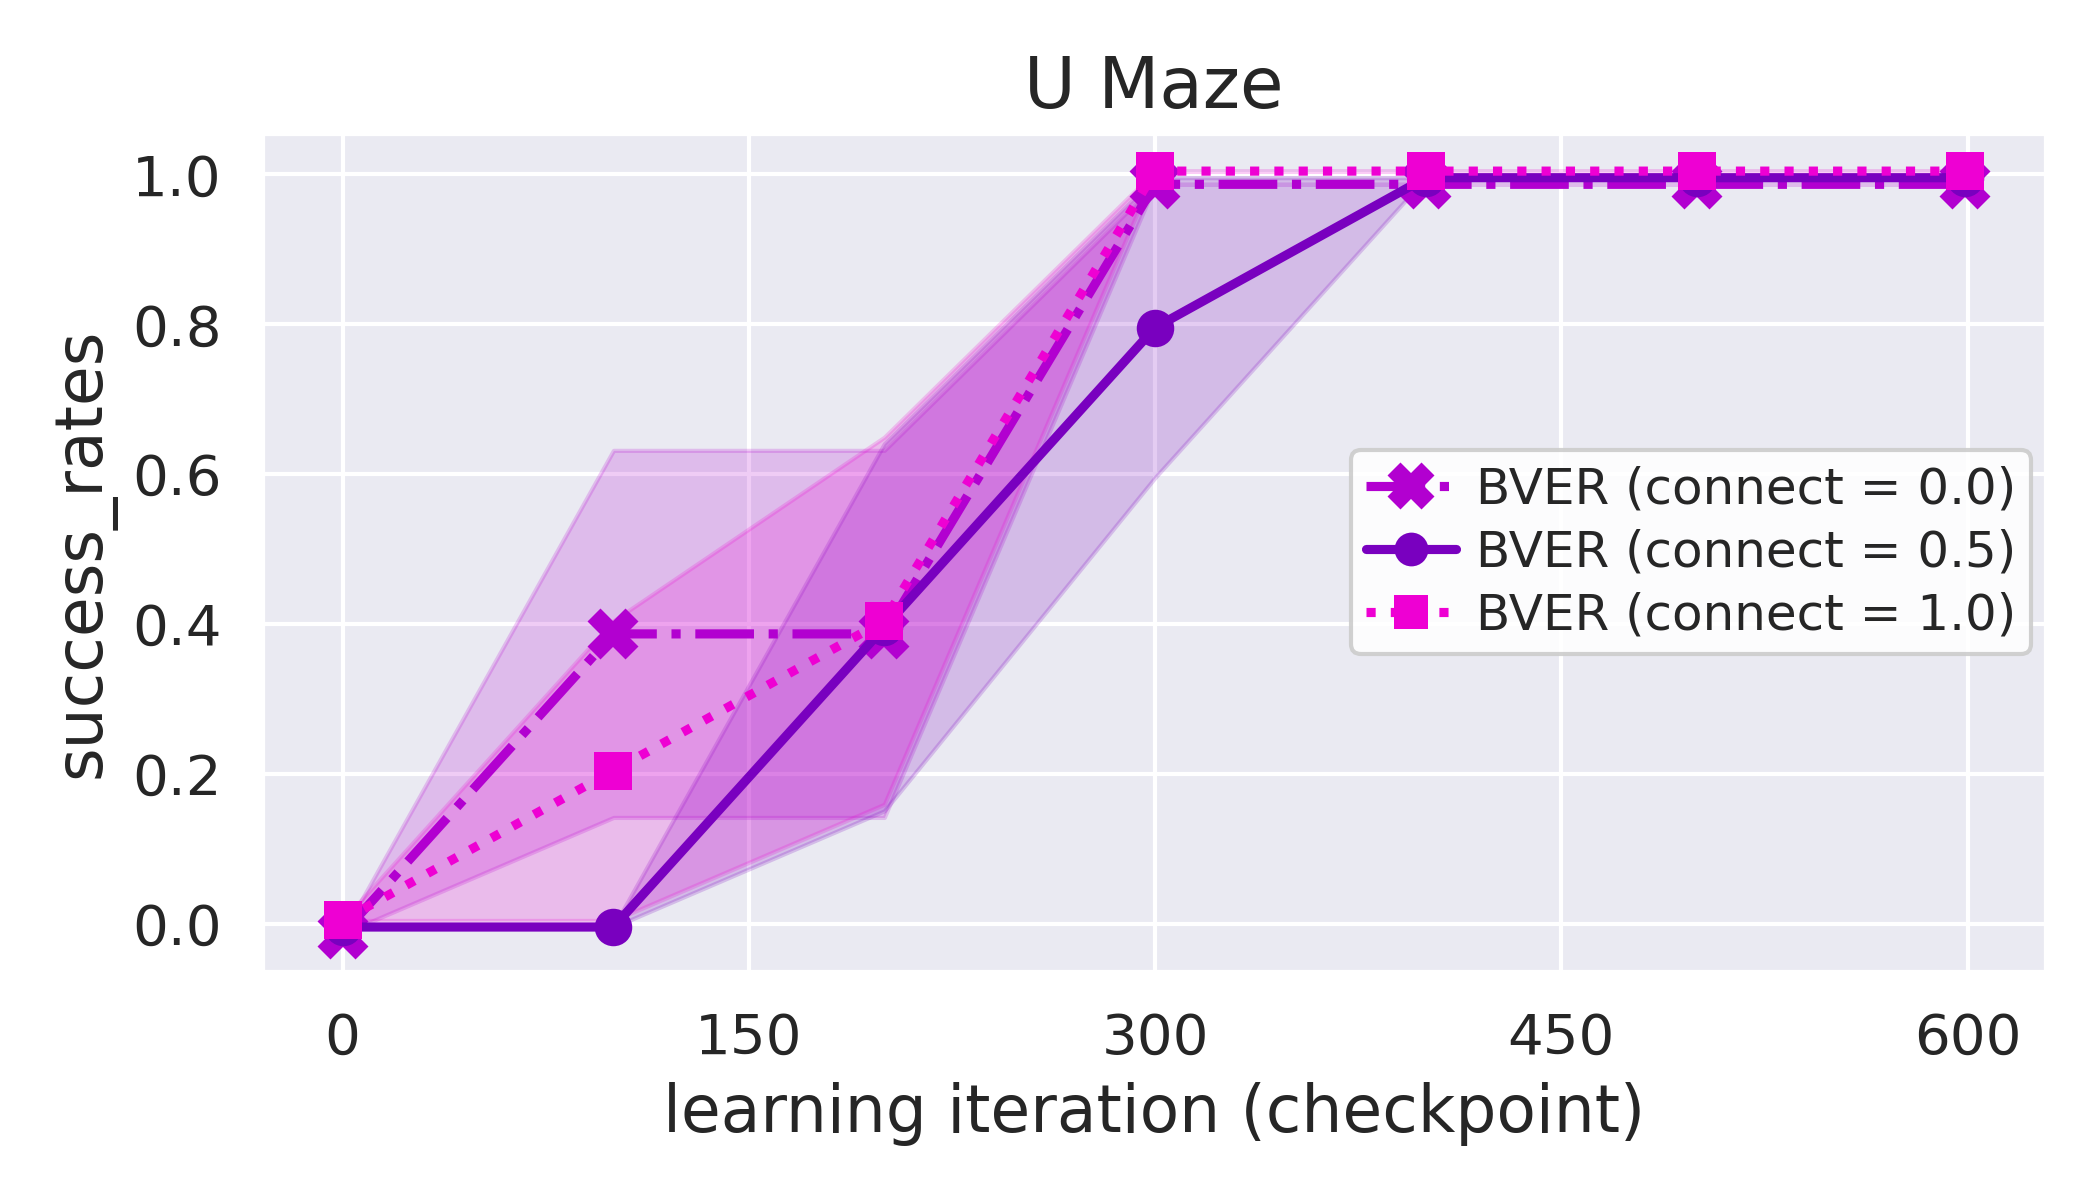
\includegraphics[width=\linewidth]{img/maze/u/eval_comparison_u_maze_abl_connect.png}
    \end{subfigure}
    %
    \hfill\strut{}\\[-2em]
    \hfill
    \begin{subfigure}[c]{0.11\linewidth}
        \centering
        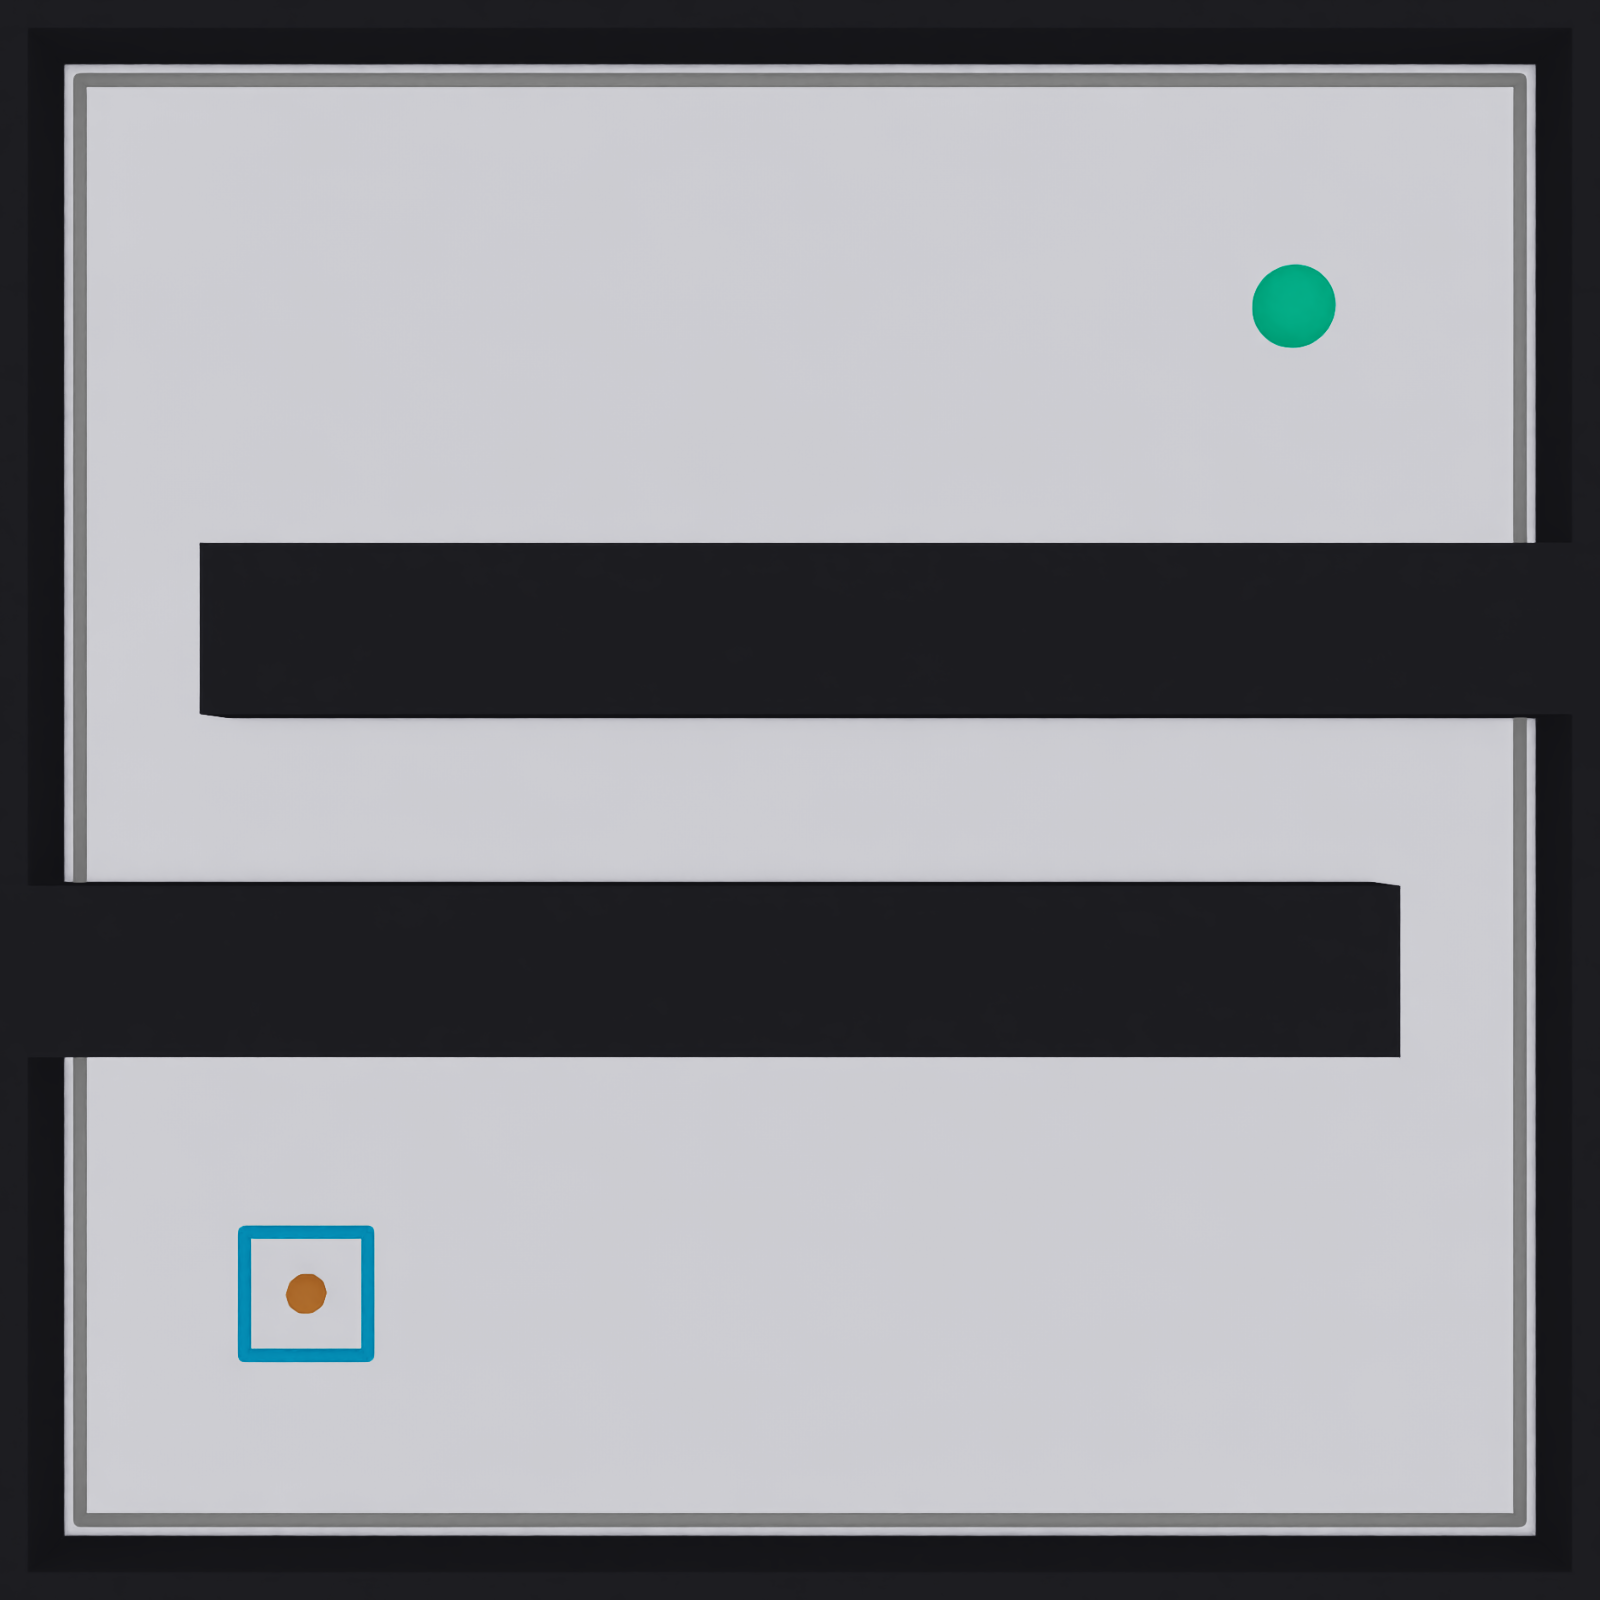
\includegraphics[width=\linewidth]{img/maze/layouts/maze_serpentine.png}
    \end{subfigure}
    \hfill
    \begin{subfigure}[c]{0.29\linewidth}
        \centering
        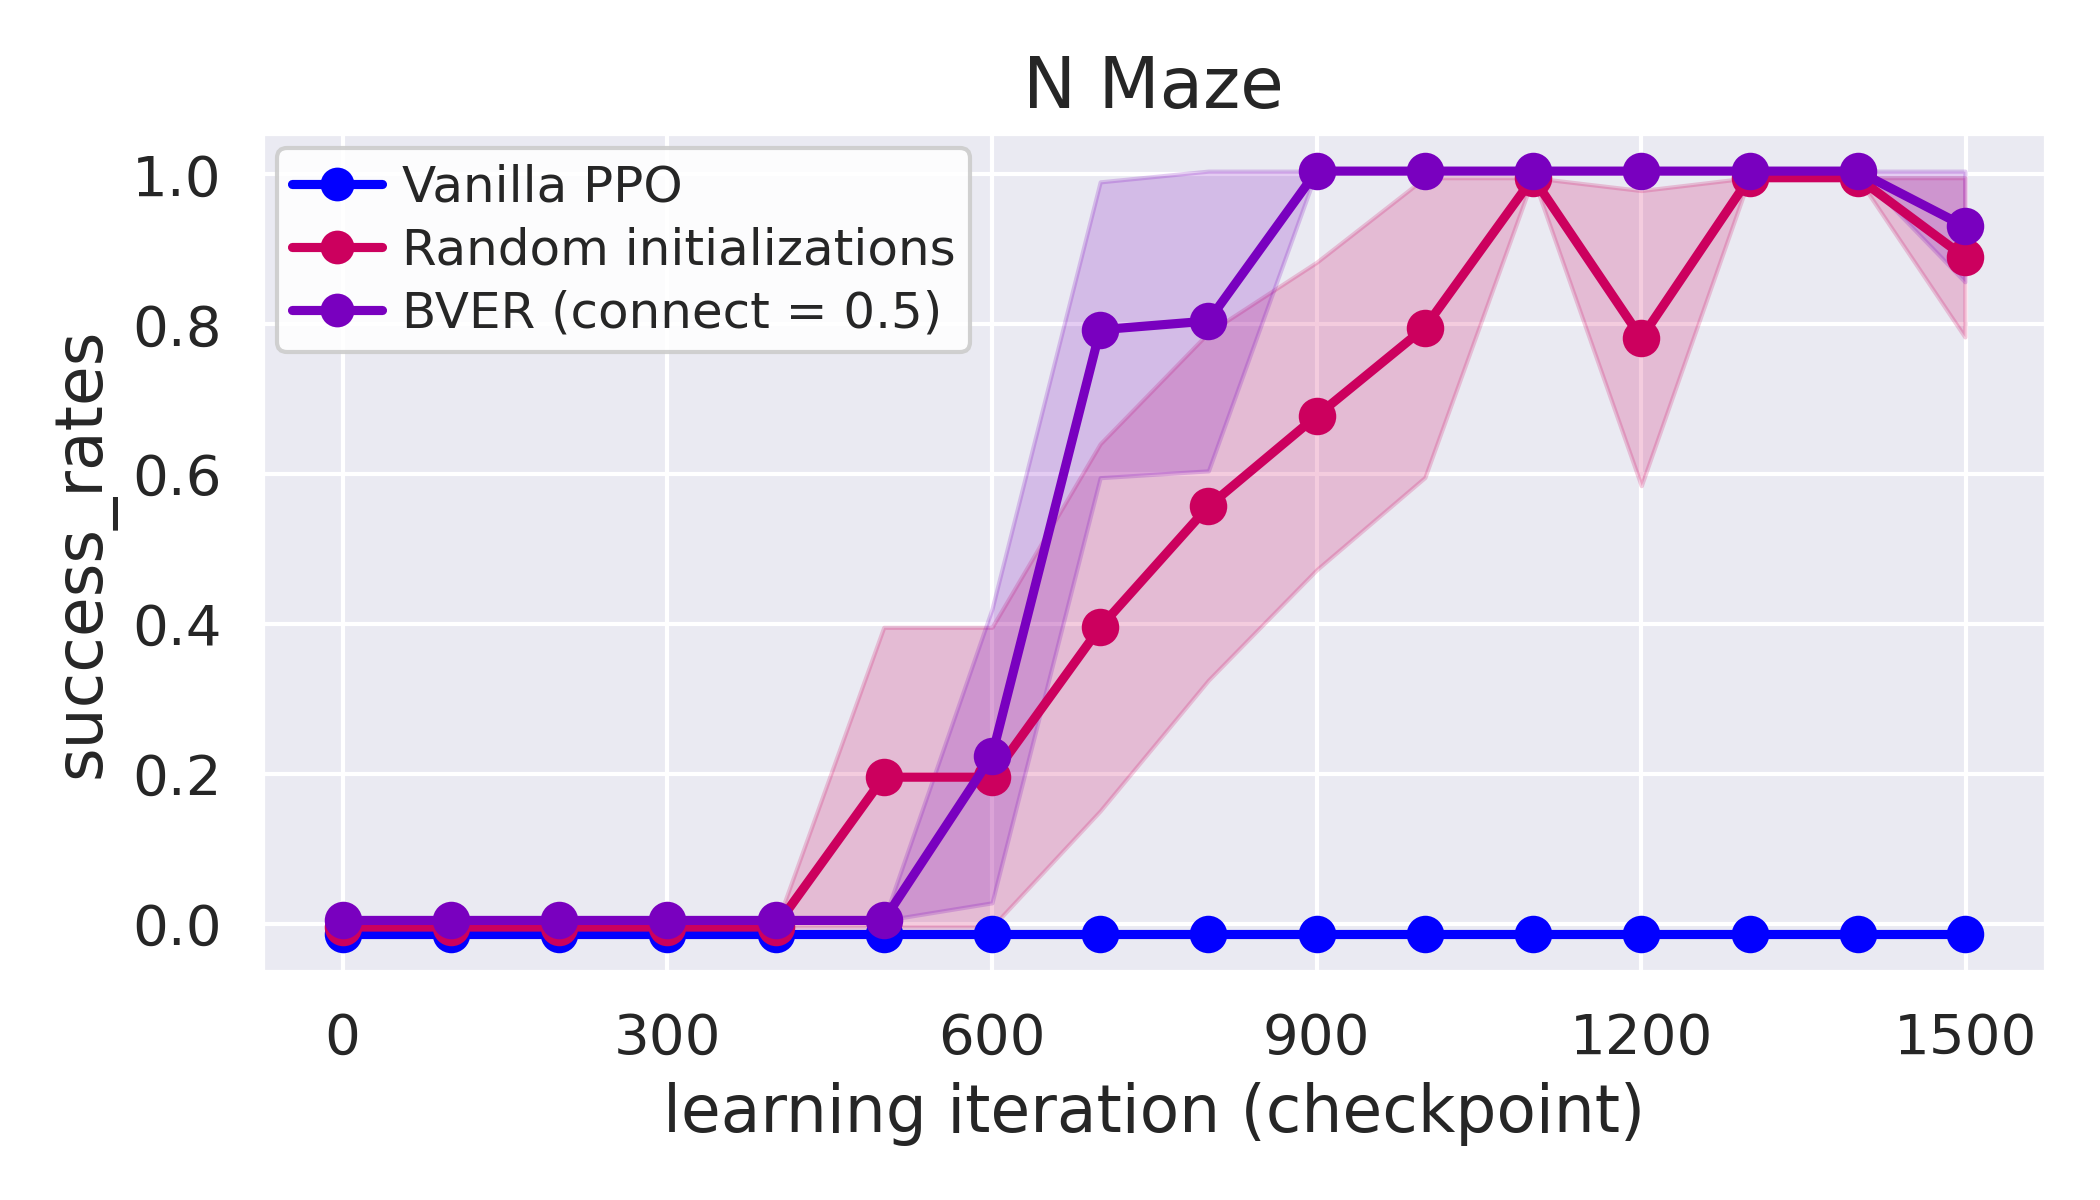
\includegraphics[width=\linewidth]{img/maze/N/eval_comparison_N_maze_bench.png}
    \end{subfigure}
    \hfill
    \begin{subfigure}[c]{0.29\linewidth}
        \centering
        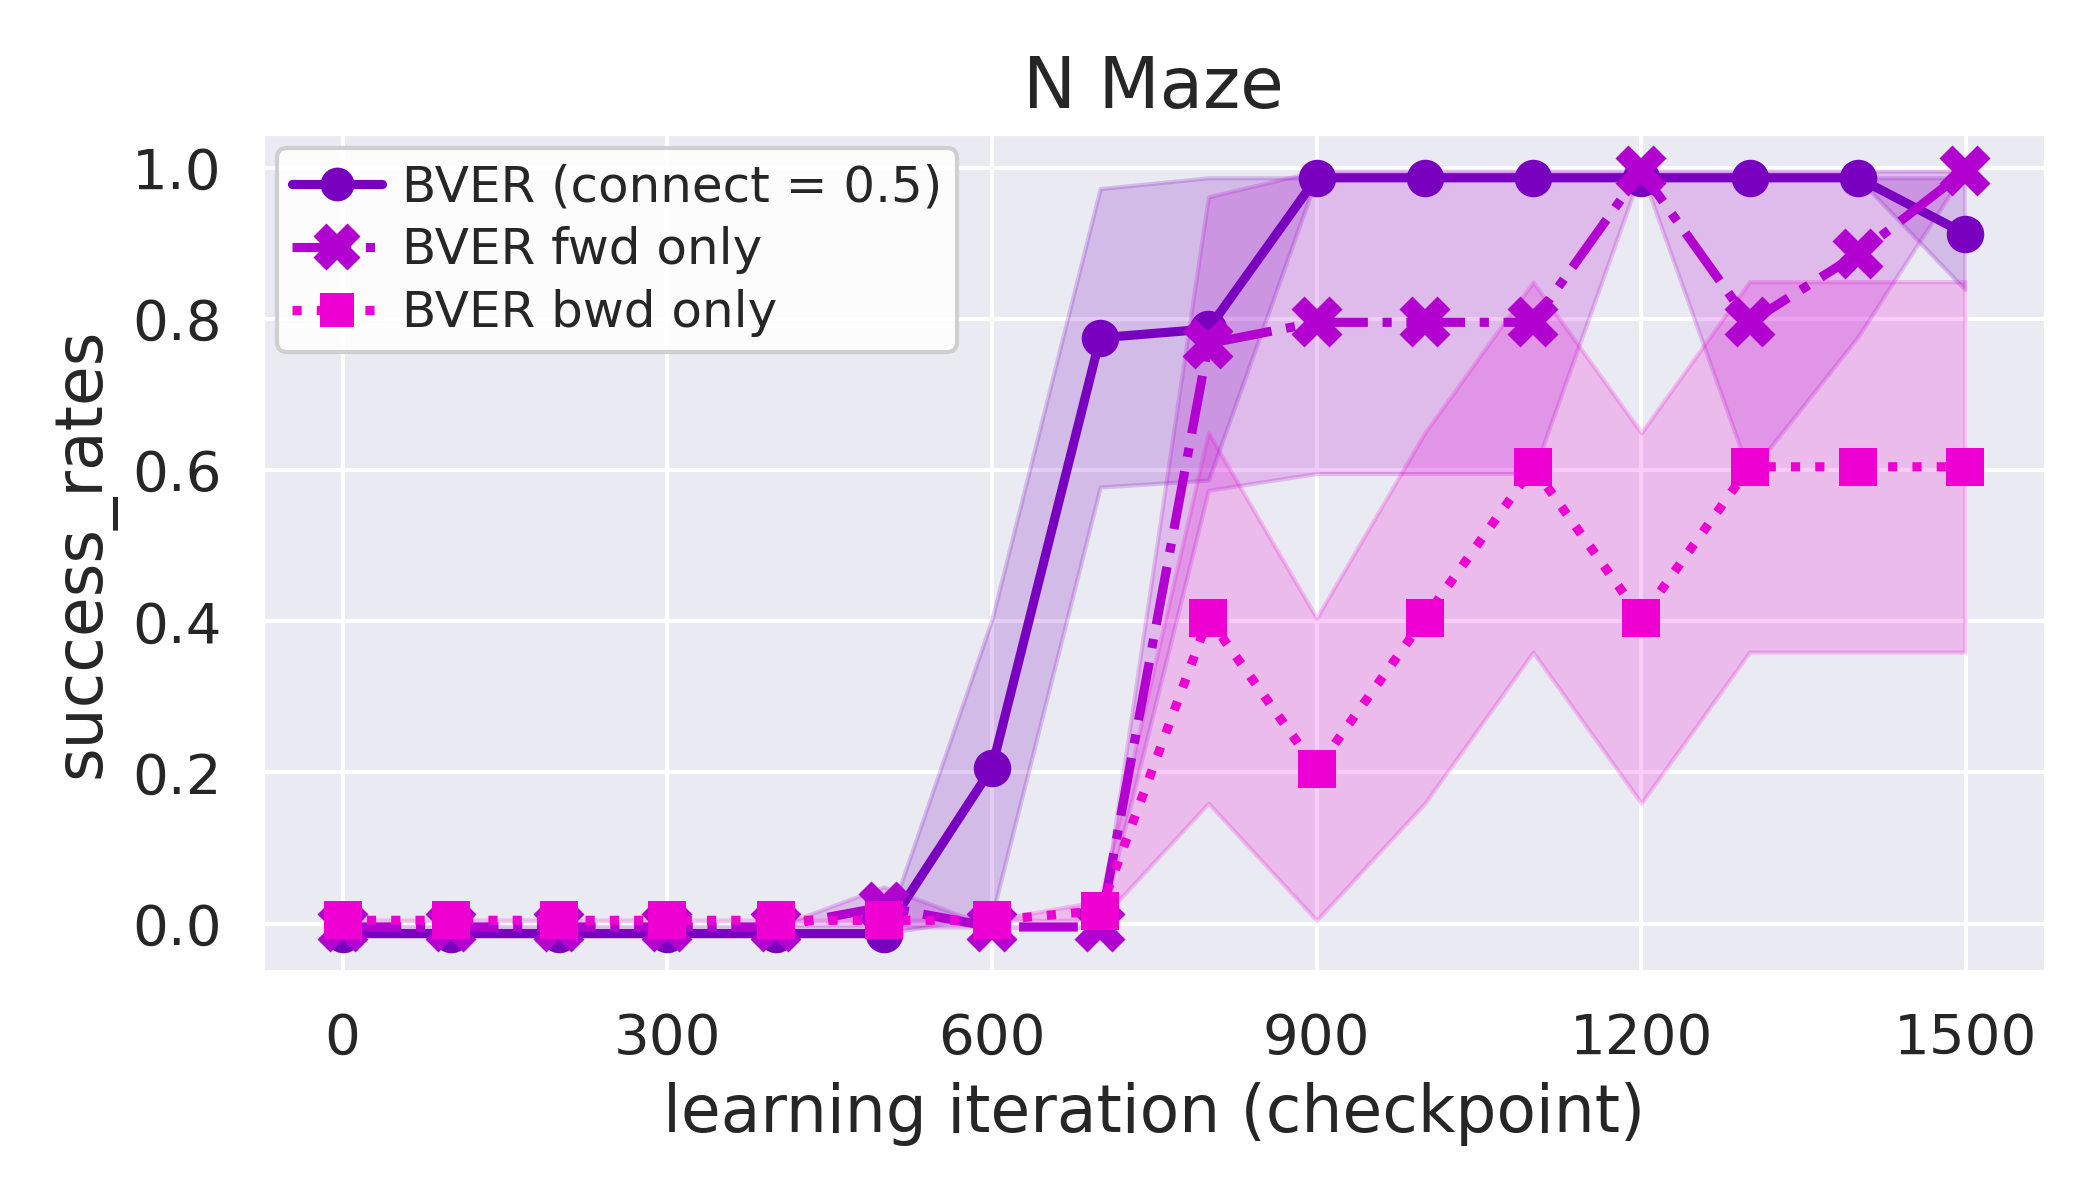
\includegraphics[width=\linewidth]{img/maze/N/eval_comparison_N_maze_abl_dir.png}
    \end{subfigure}
    \hfill
    \begin{subfigure}[c]{0.29\linewidth}
        \centering
        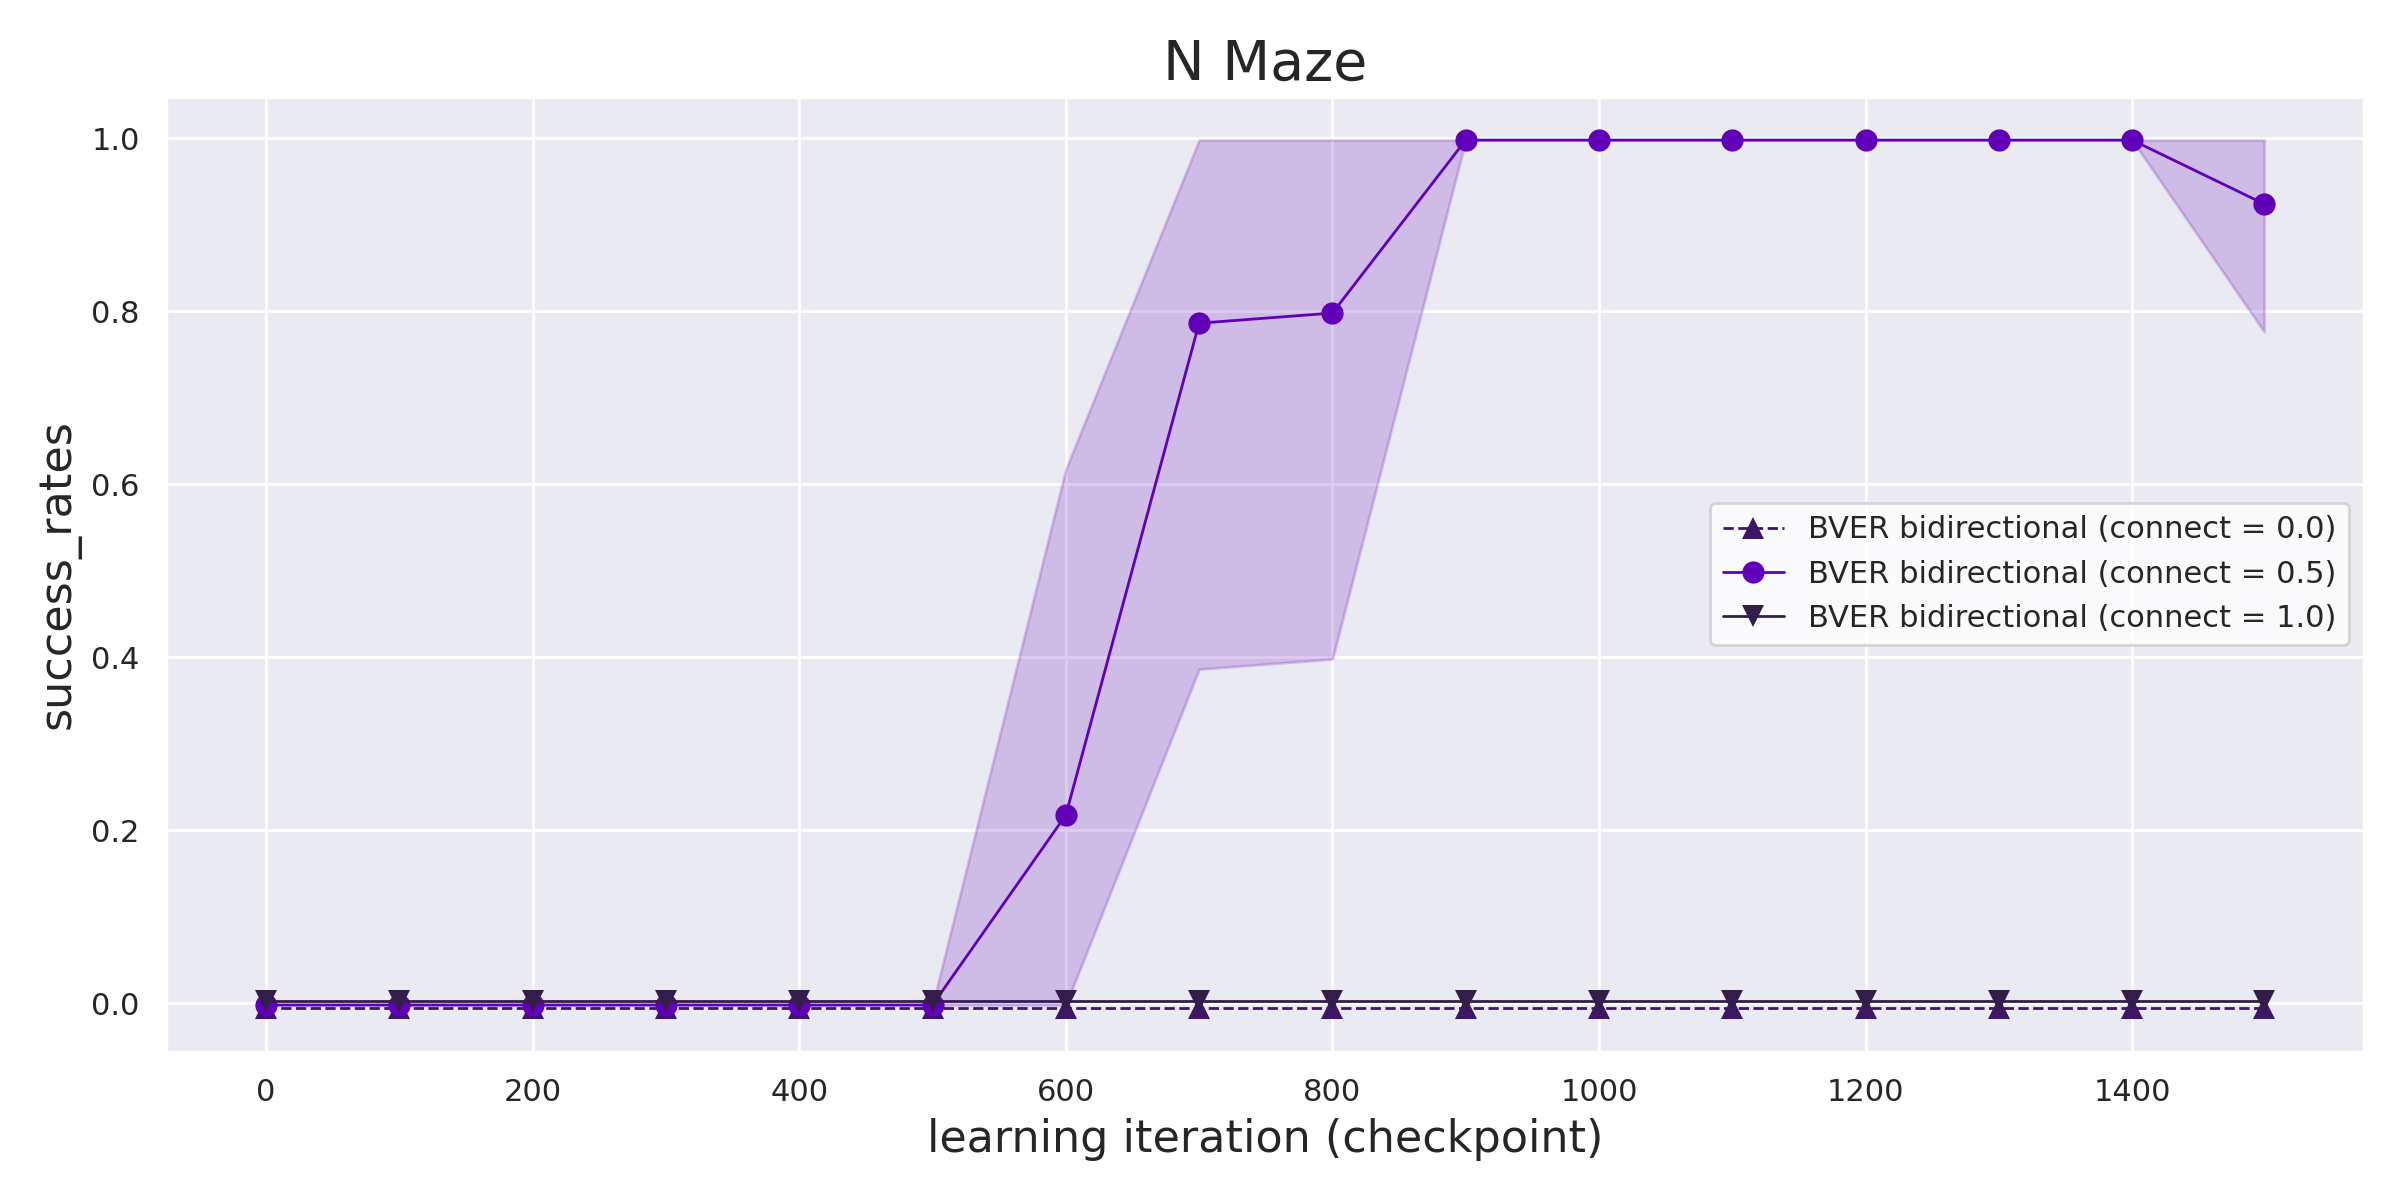
\includegraphics[width=\linewidth]{img/maze/N/eval_comparison_N_maze_abl_connect.png}
    \end{subfigure}
    \hfill\strut{}\\[-2em]
    %
    \hfill
    \begin{subfigure}[c]{0.11\linewidth}
        \centering
        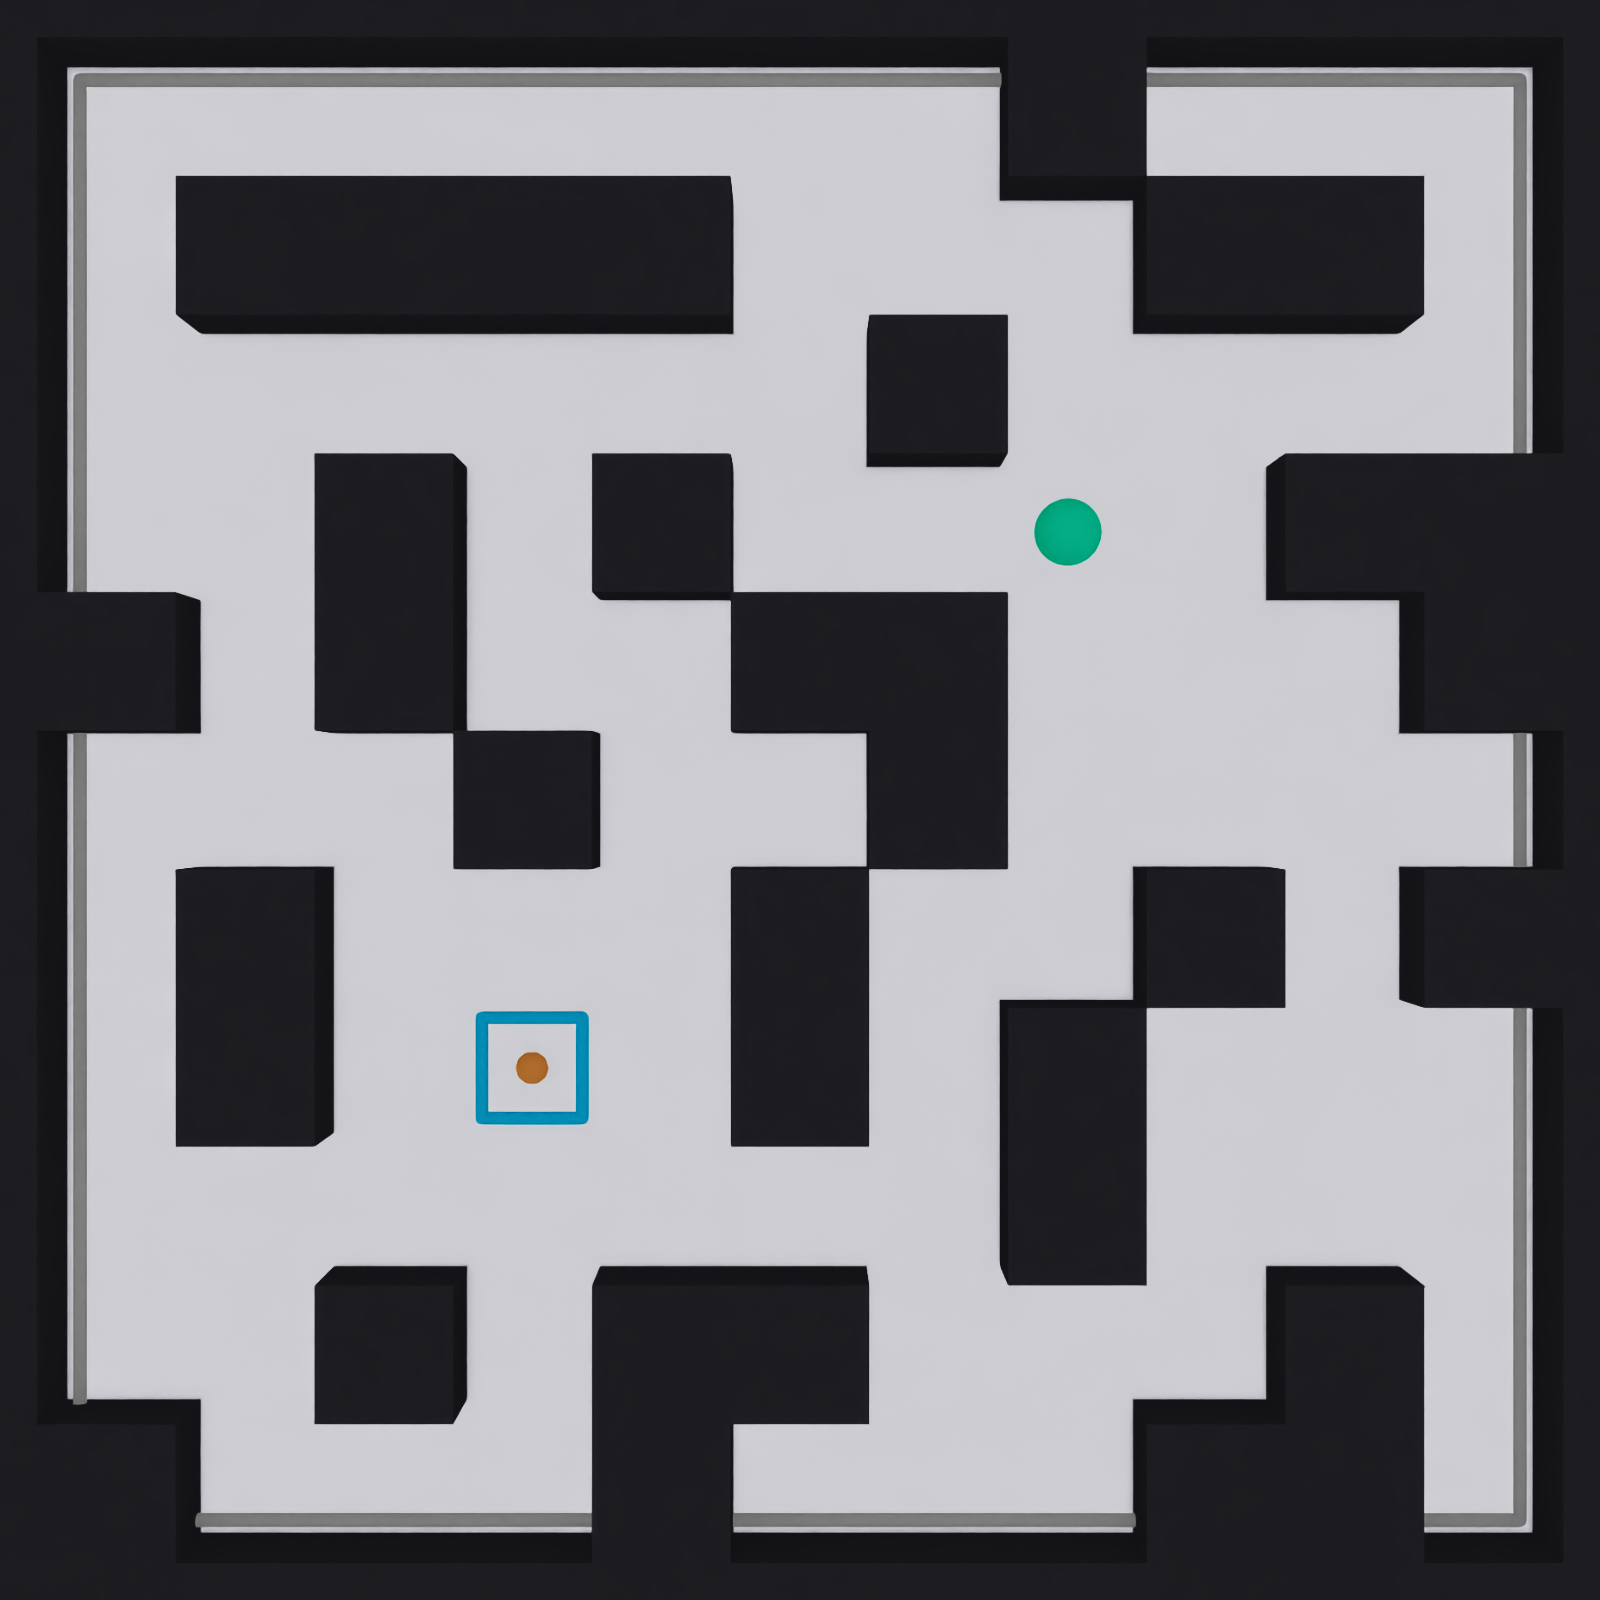
\includegraphics[width=\linewidth]{img/maze/layouts/maze_scatter.png}
        \caption{Maze layout.}\label{fig:maze_layout}
    \end{subfigure}
    \hfill
    \begin{subfigure}[c]{0.29\linewidth}
        \centering
        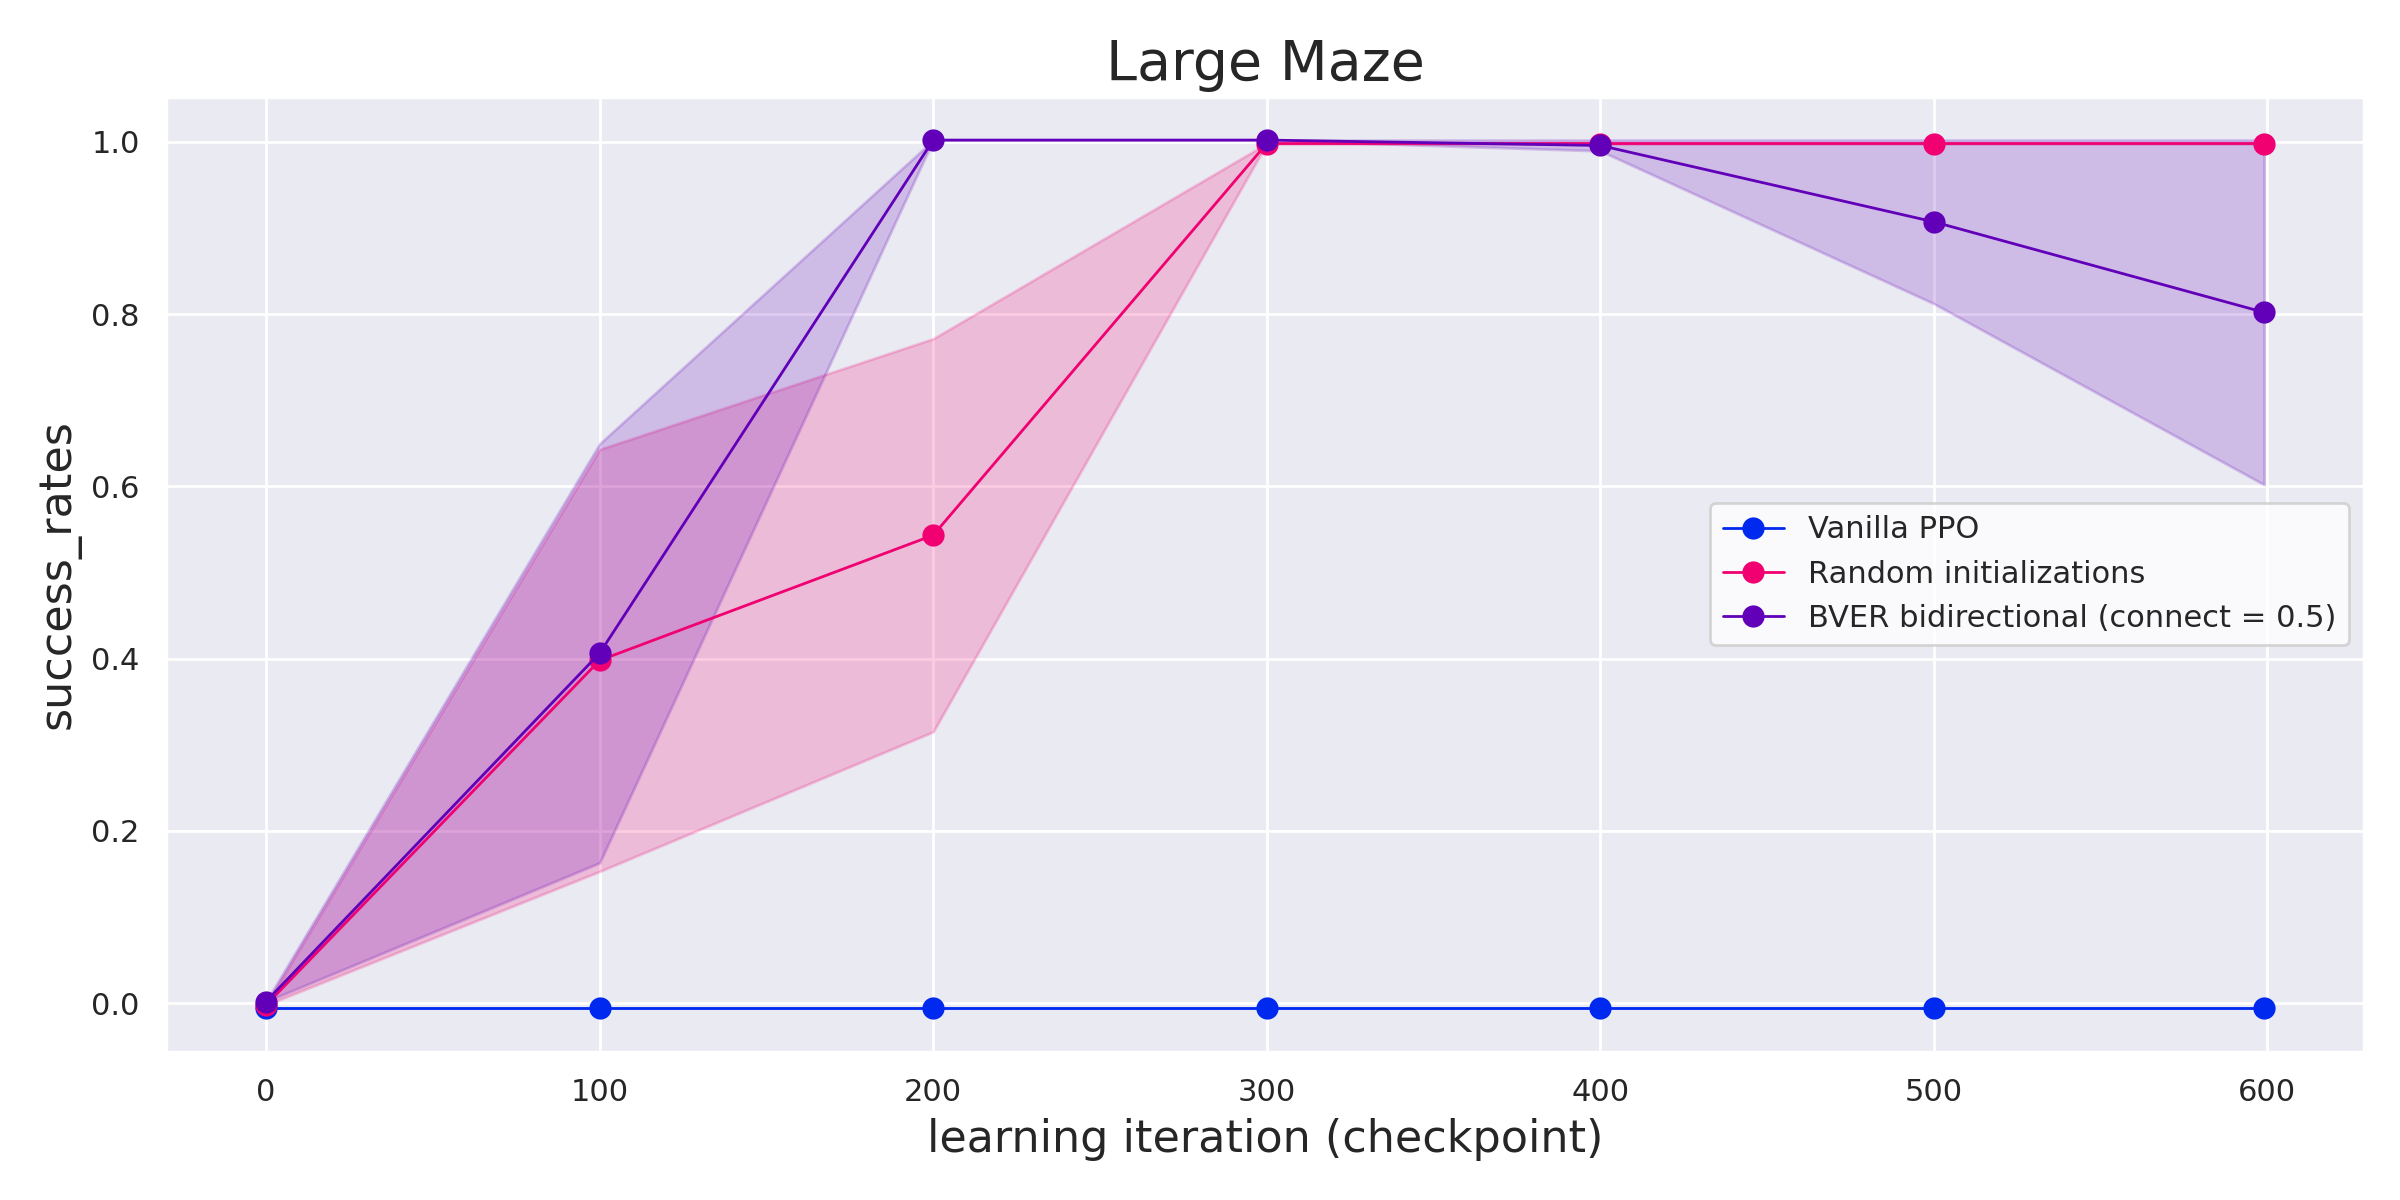
\includegraphics[width=\linewidth]{img/maze/large/eval_comparison_large_maze_bench.png}
        \caption{Benchmark.}\label{fig:maze_ablation_bench}
    \end{subfigure}
    \hfill
    \begin{subfigure}[c]{0.29\linewidth}
        \centering
        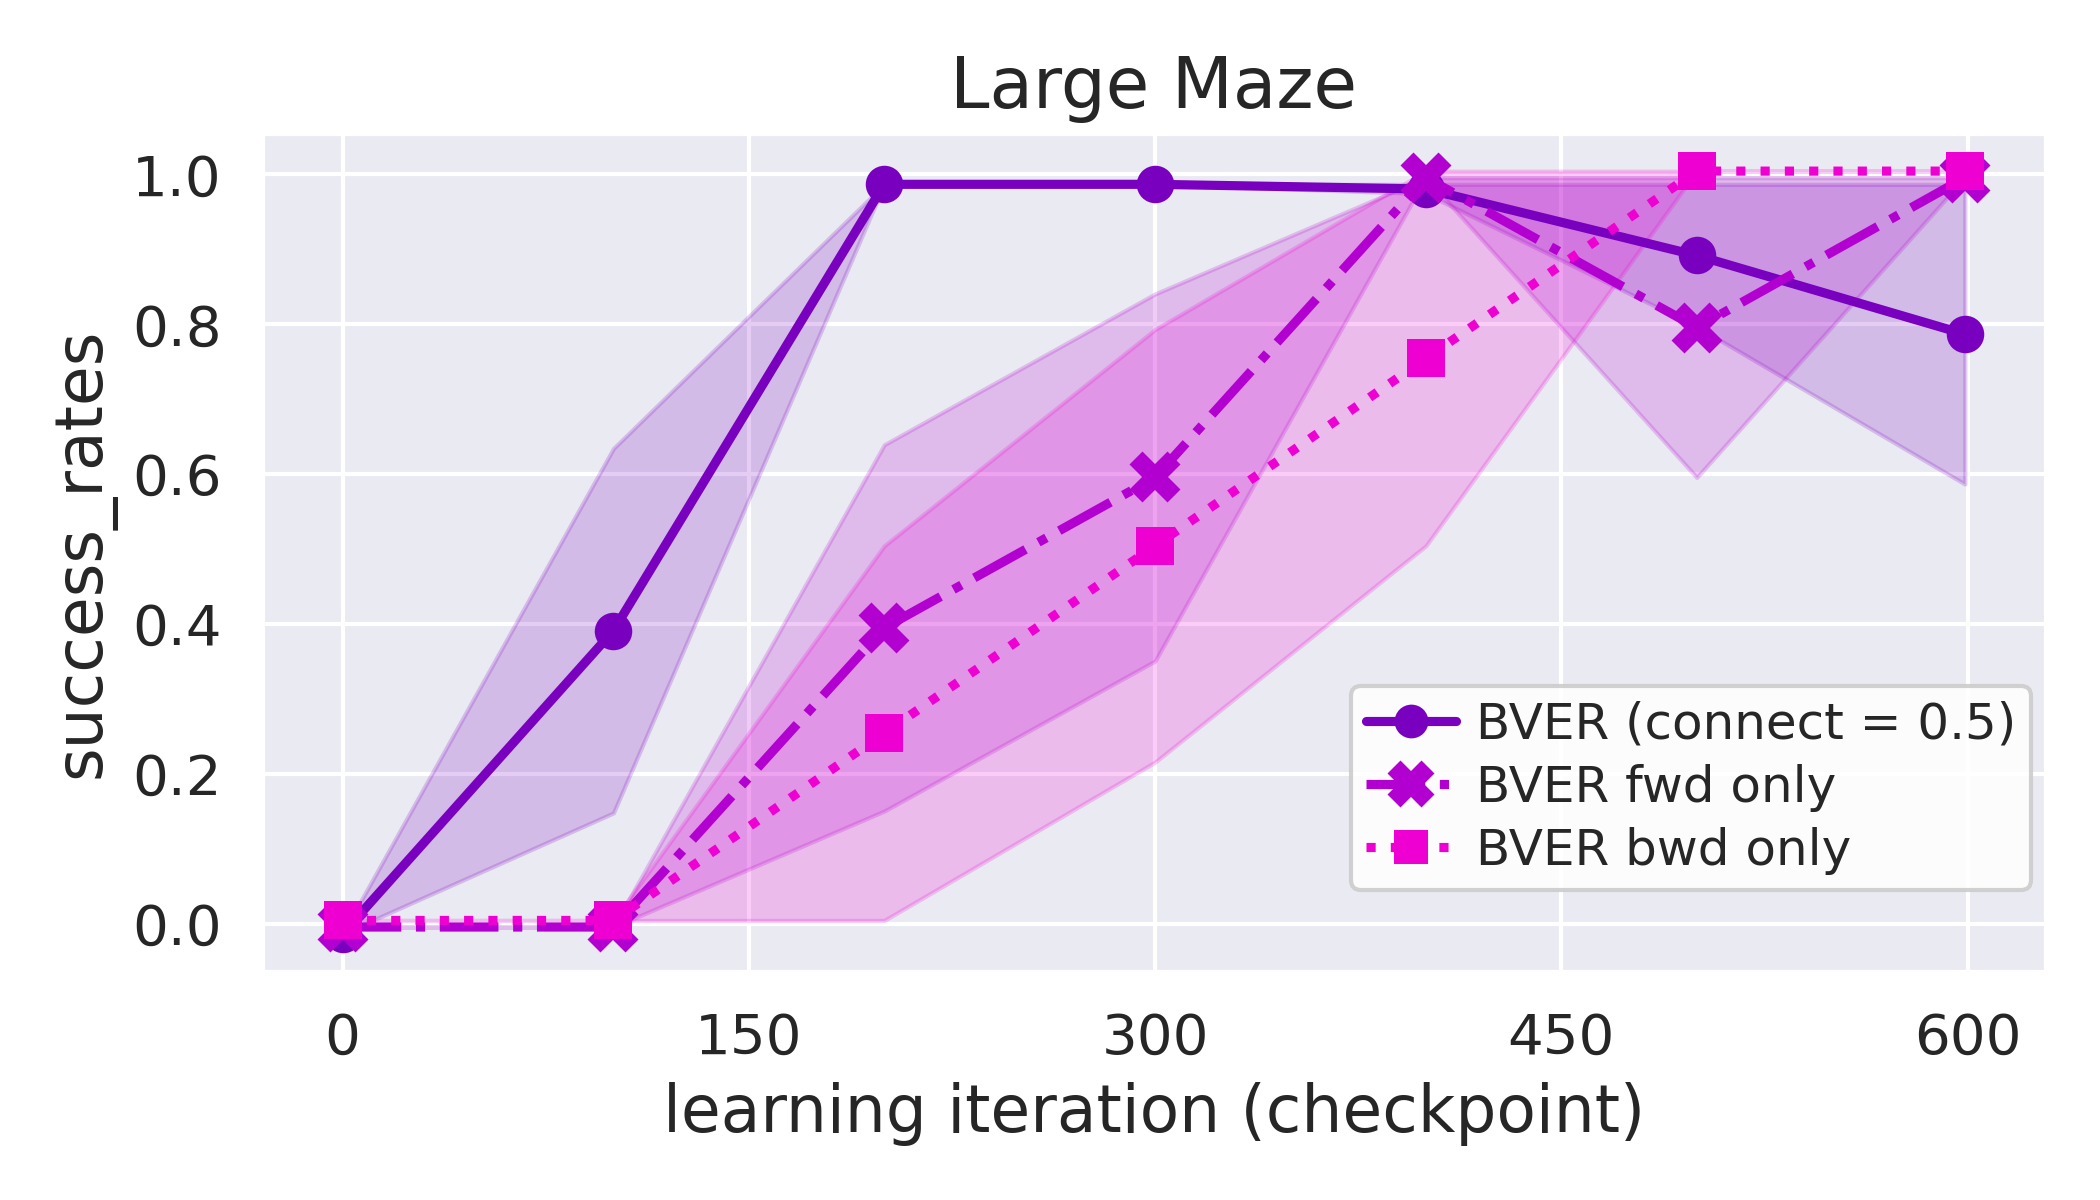
\includegraphics[width=\linewidth]{img/maze/large/eval_comparison_large_maze_abl_dir.png}
        \caption{Direction ablation.}\label{fig:maze_ablation_dir}
    \end{subfigure}
    \hfill
    \begin{subfigure}[c]{0.29\linewidth}
        \centering
        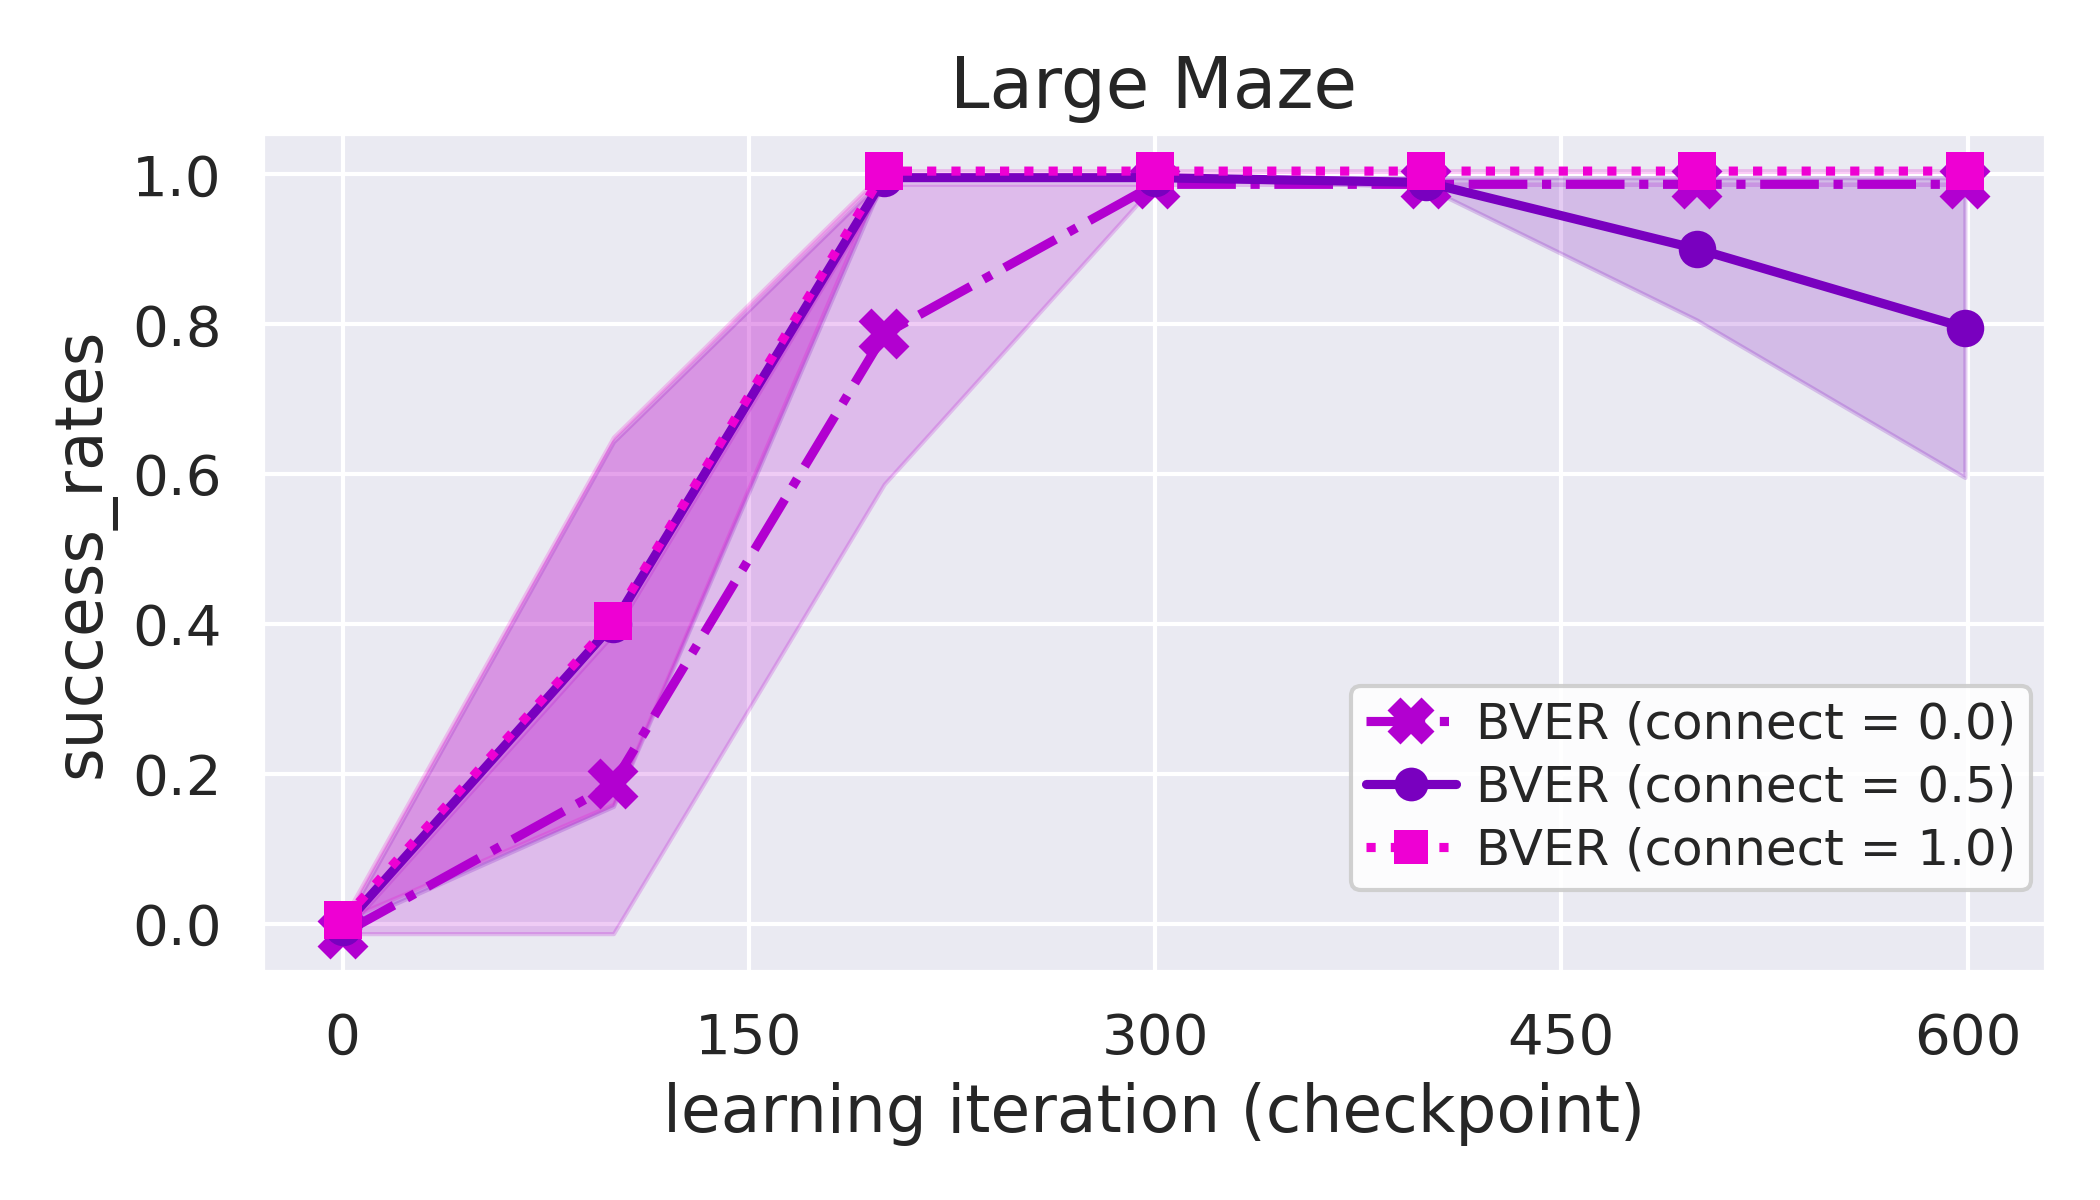
\includegraphics[width=\linewidth]{img/maze/large/eval_comparison_large_maze_abl_connect.png}
        \caption{Connect ablation.}\label{fig:maze_ablation_connect}
    \end{subfigure}
    \hfill\strut{}
    \caption{Comparison of BVER against vanilla PPO and a random curriculum, and ablations of different components (expansion directions) and hyperparameters (connect ratio).}\label{fig:eval_maze_ablations}
\end{figure}

\begin{wrapfigure}{r}{0.55\linewidth}
    \centering
    \vspace{-\baselineskip}
    \begin{subfigure}[b]{0.48\linewidth}
        \centering
        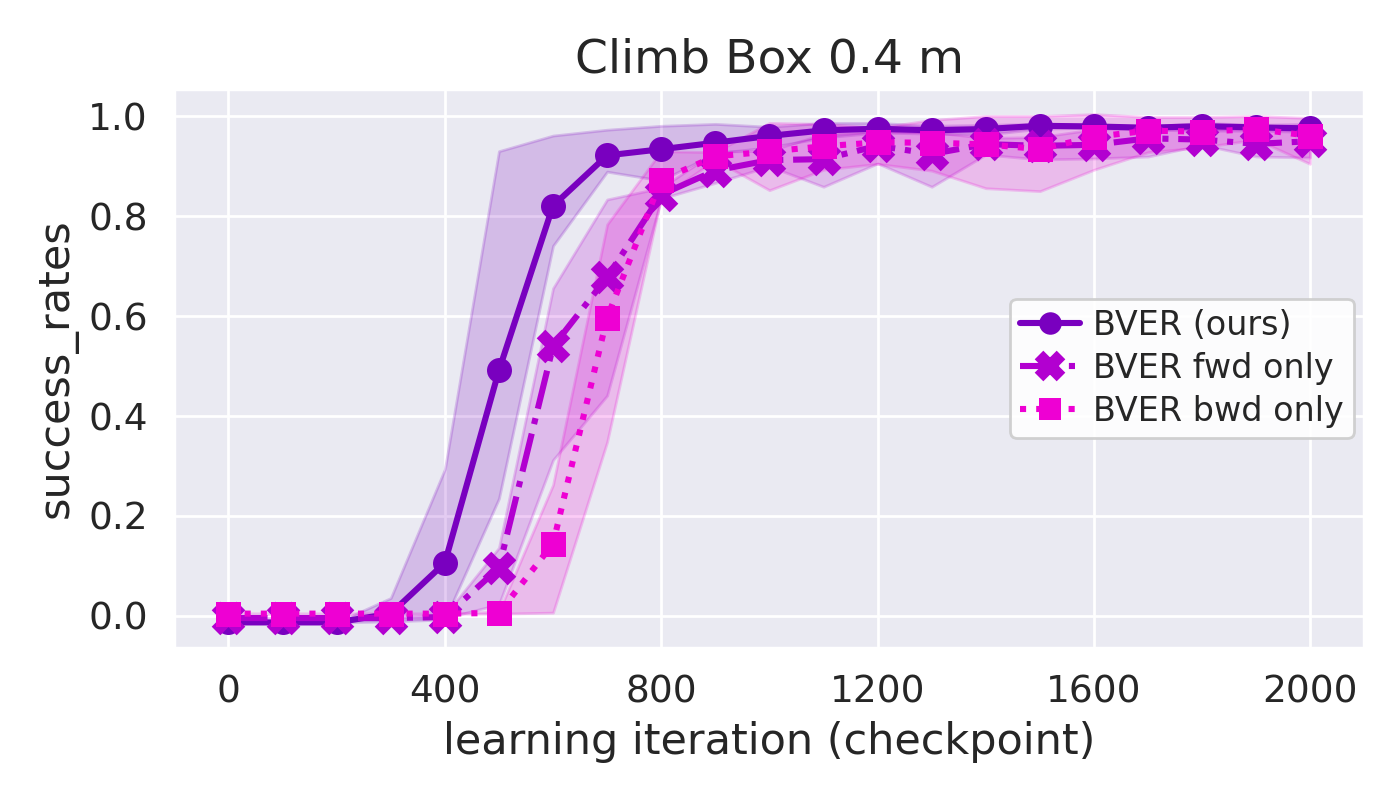
\includegraphics[width=\linewidth]{img/sb/eval_comparison_41_up_ours.png}
        \caption{Climb 0.4 m box up.}\label{fig:eval_comparison_41_up_ours}
    \end{subfigure}
    \hfill
    \begin{subfigure}[b]{0.48\linewidth}
        \centering
        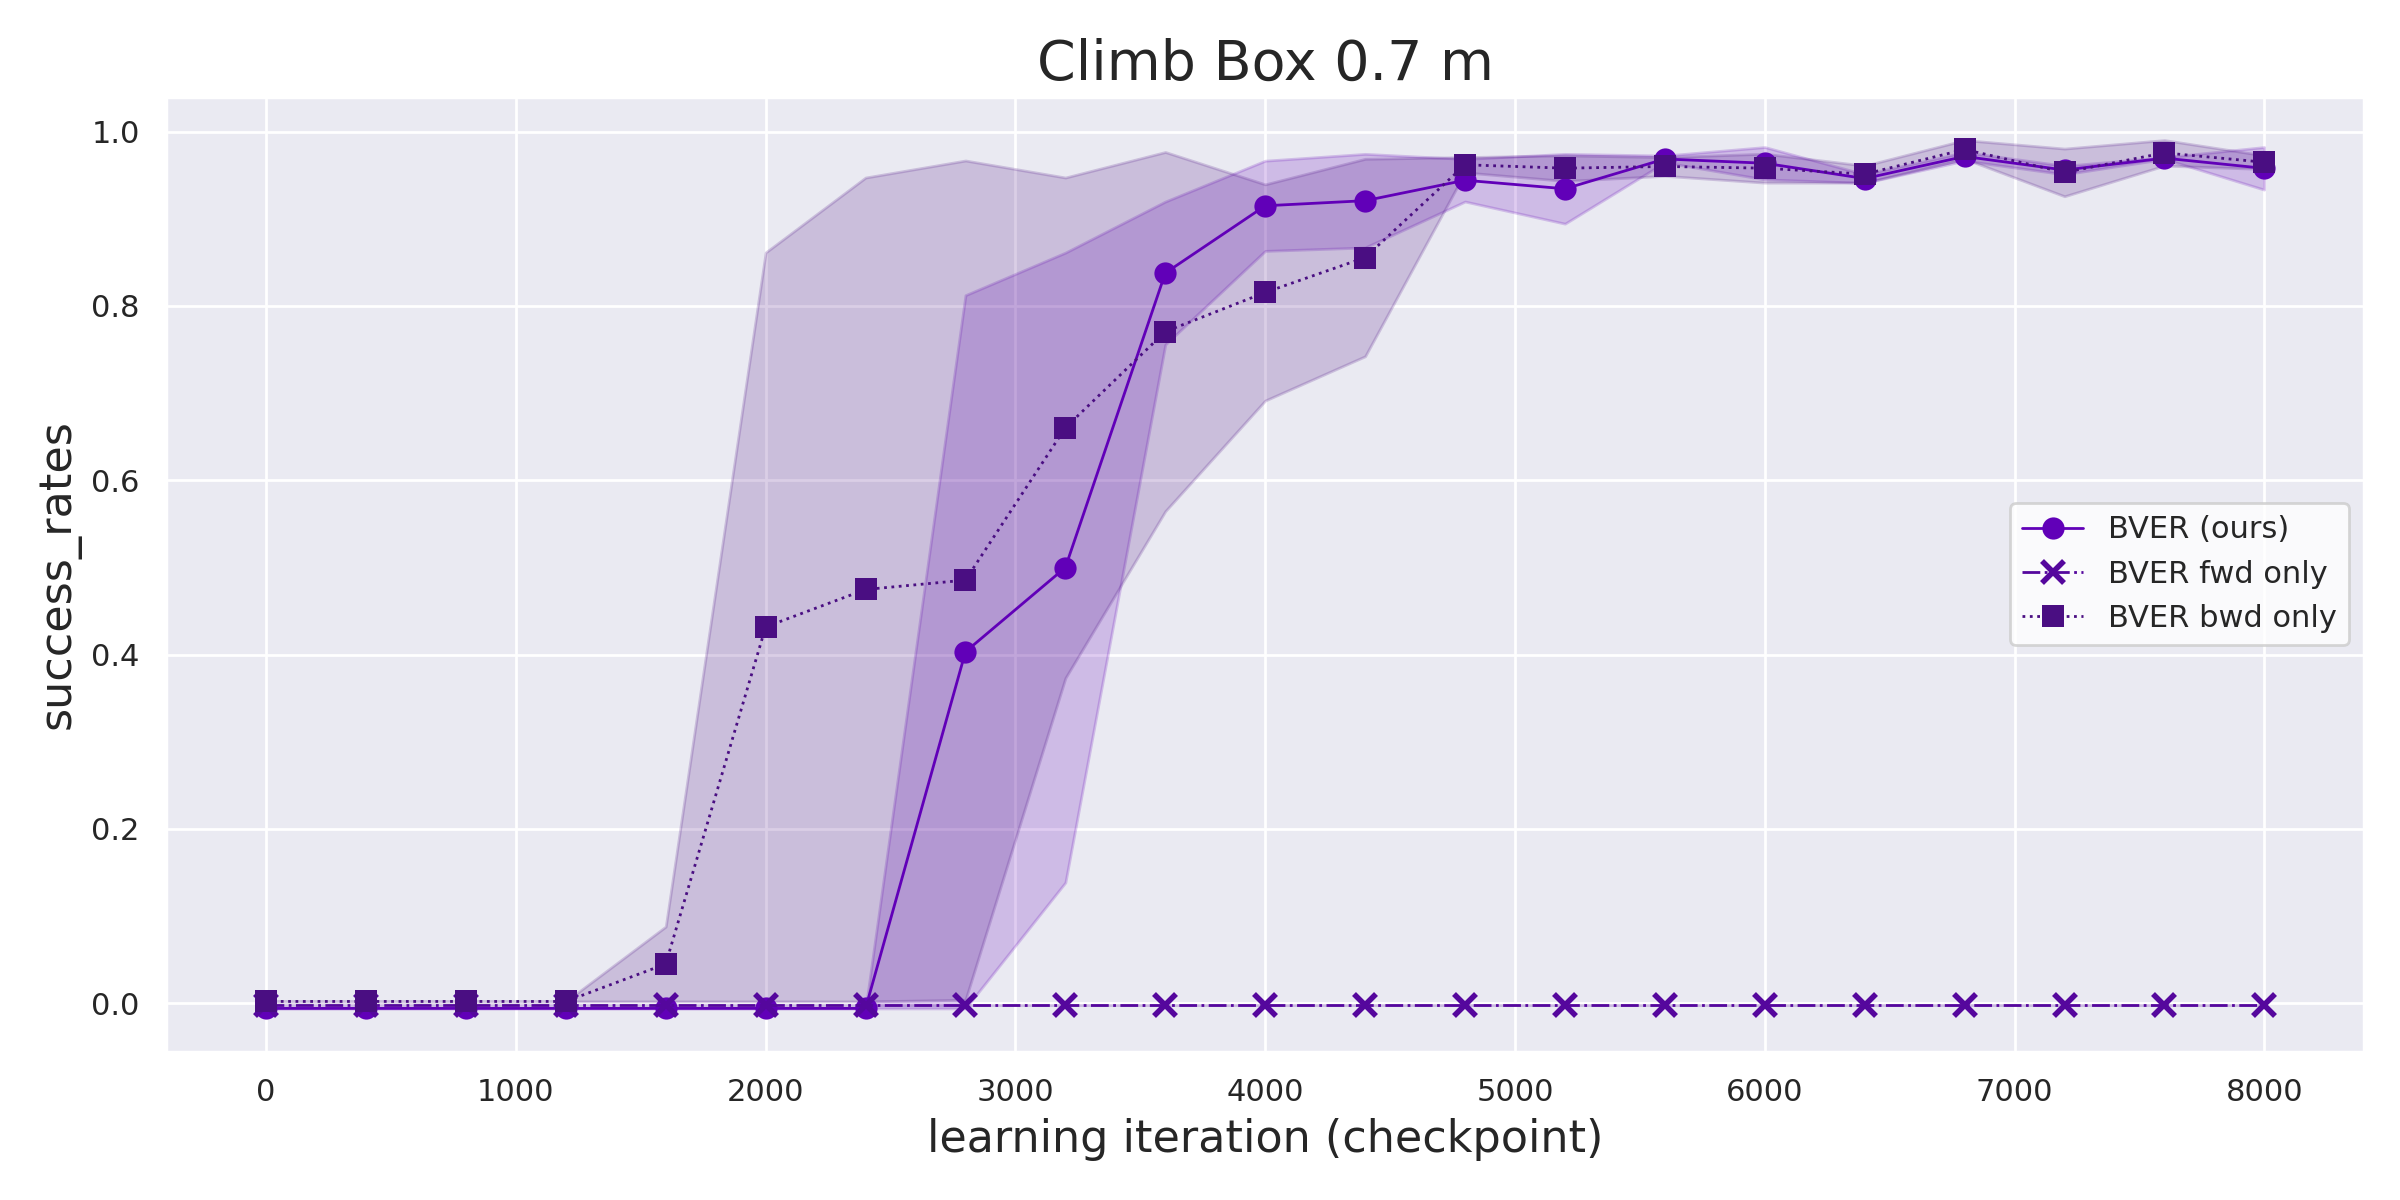
\includegraphics[width=\linewidth]{img/sb/eval_comparison_72_up_ours.png}
        \caption{Climb 0.7 m box up.}\label{fig:eval_comparison_72_up_ours}
    \end{subfigure}
    \\[1ex]
    \begin{subfigure}[b]{0.48\linewidth}
        \centering
        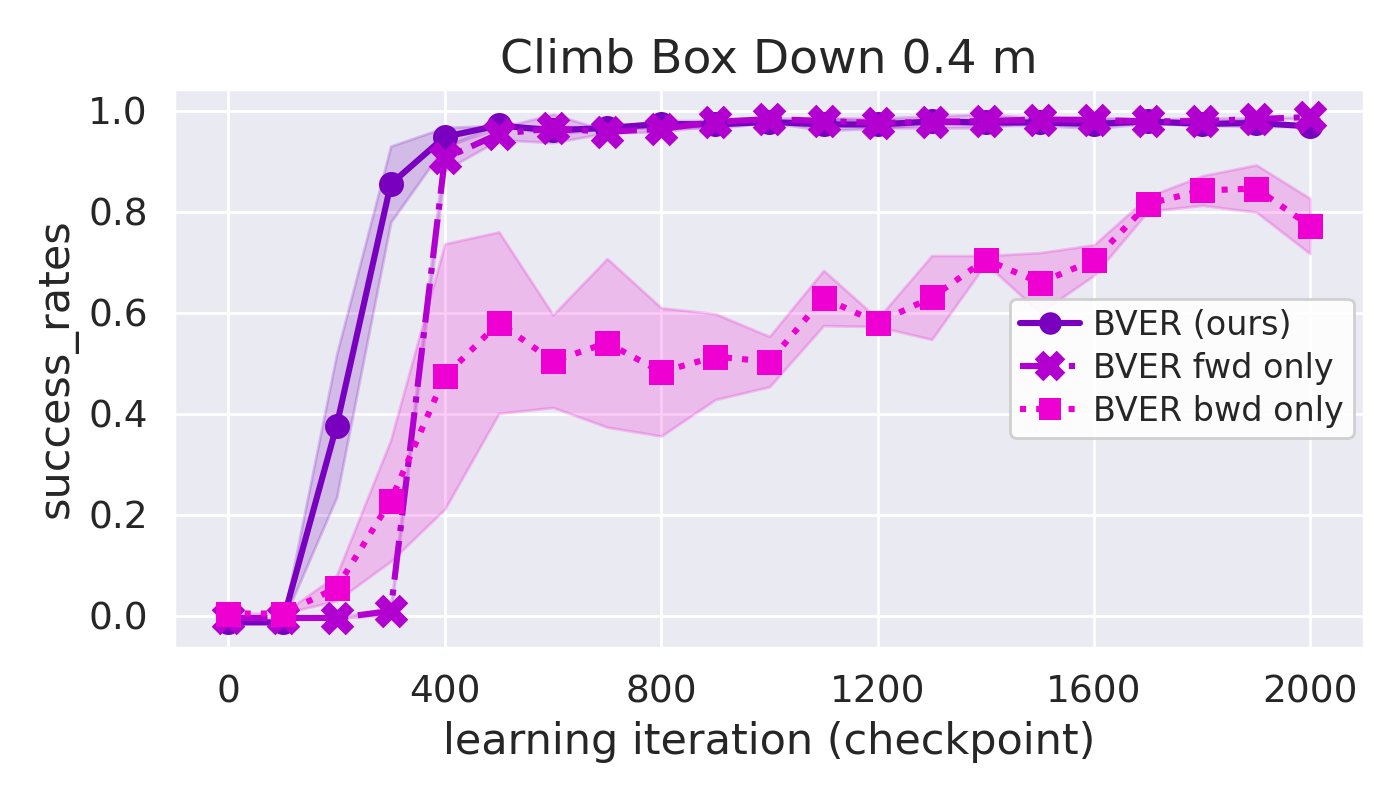
\includegraphics[width=\linewidth]{img/sb/eval_comparison_41_down_ours.png}
        \caption{Climb 0.4 m box down.}\label{fig:eval_comparison_41_down_ours}
    \end{subfigure}
    \hfill
    \begin{subfigure}[b]{0.48\linewidth}
        \centering
        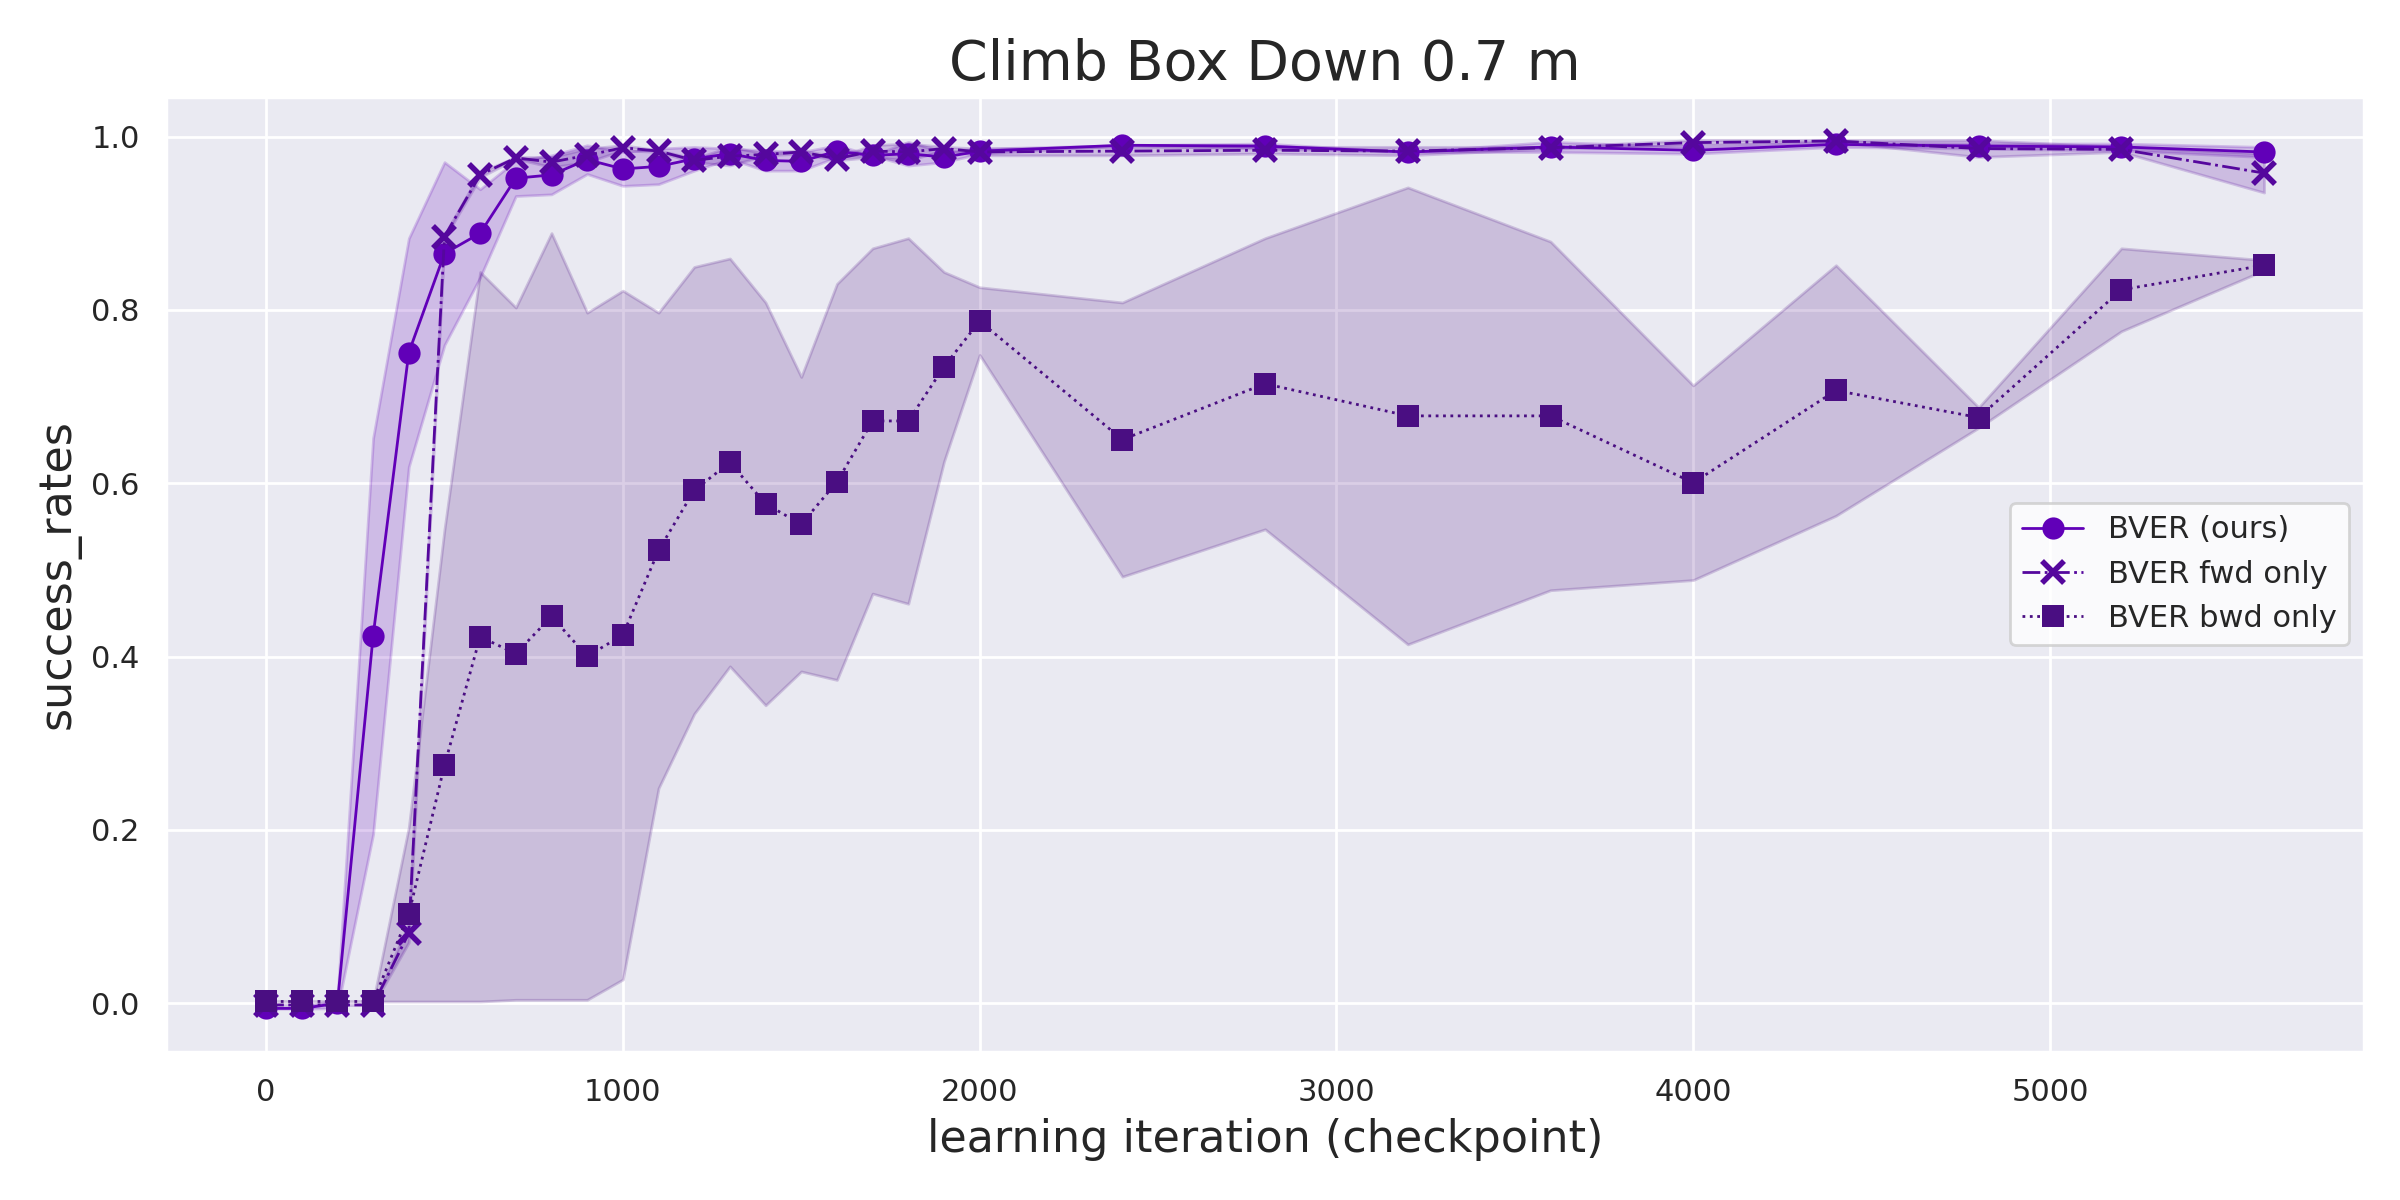
\includegraphics[width=\linewidth]{img/sb/eval_comparison_72_down_ours.png}
        \caption{Climb 0.7 m box down.}\label{fig:eval_comparison_72_down_ours}
    \end{subfigure}
    \caption{Ablations on the box climbing task show that combining forwards and backwards expansions leads to the best results irrespective of direction (up or down) and box height.}\label{fig:eval_ablations}
\end{wrapfigure}
\paragraph{Box climbing ablations:}
We evaluate the effect of the bidirectional expansion mechanism by comparing BVER on two symmetric climbing tasks (up and down) against its unidirectional variants, i.e., only expanding the curriculum from the start state (forwards expansion) or only expanding the curriculum from the goal state (backwards expansion). The results in Figure~\ref{fig:eval_ablations} show that combining forwards and backwards expansions leads to the best results irrespective of the task (up or down) and box height. In both tasks, the expansion that starts on top of the box performs better than the one that starts on the ground. This is likely because the random walks are subject to gravity, so traversing down the box edge is more likely than traversing up it.


\subsection{Emergent Behavior: Path Diversity}\label{sec:exp_emergent}

\begin{wrapfigure}{r}{0.4\linewidth}
    \centering
    \vspace{-\baselineskip}
    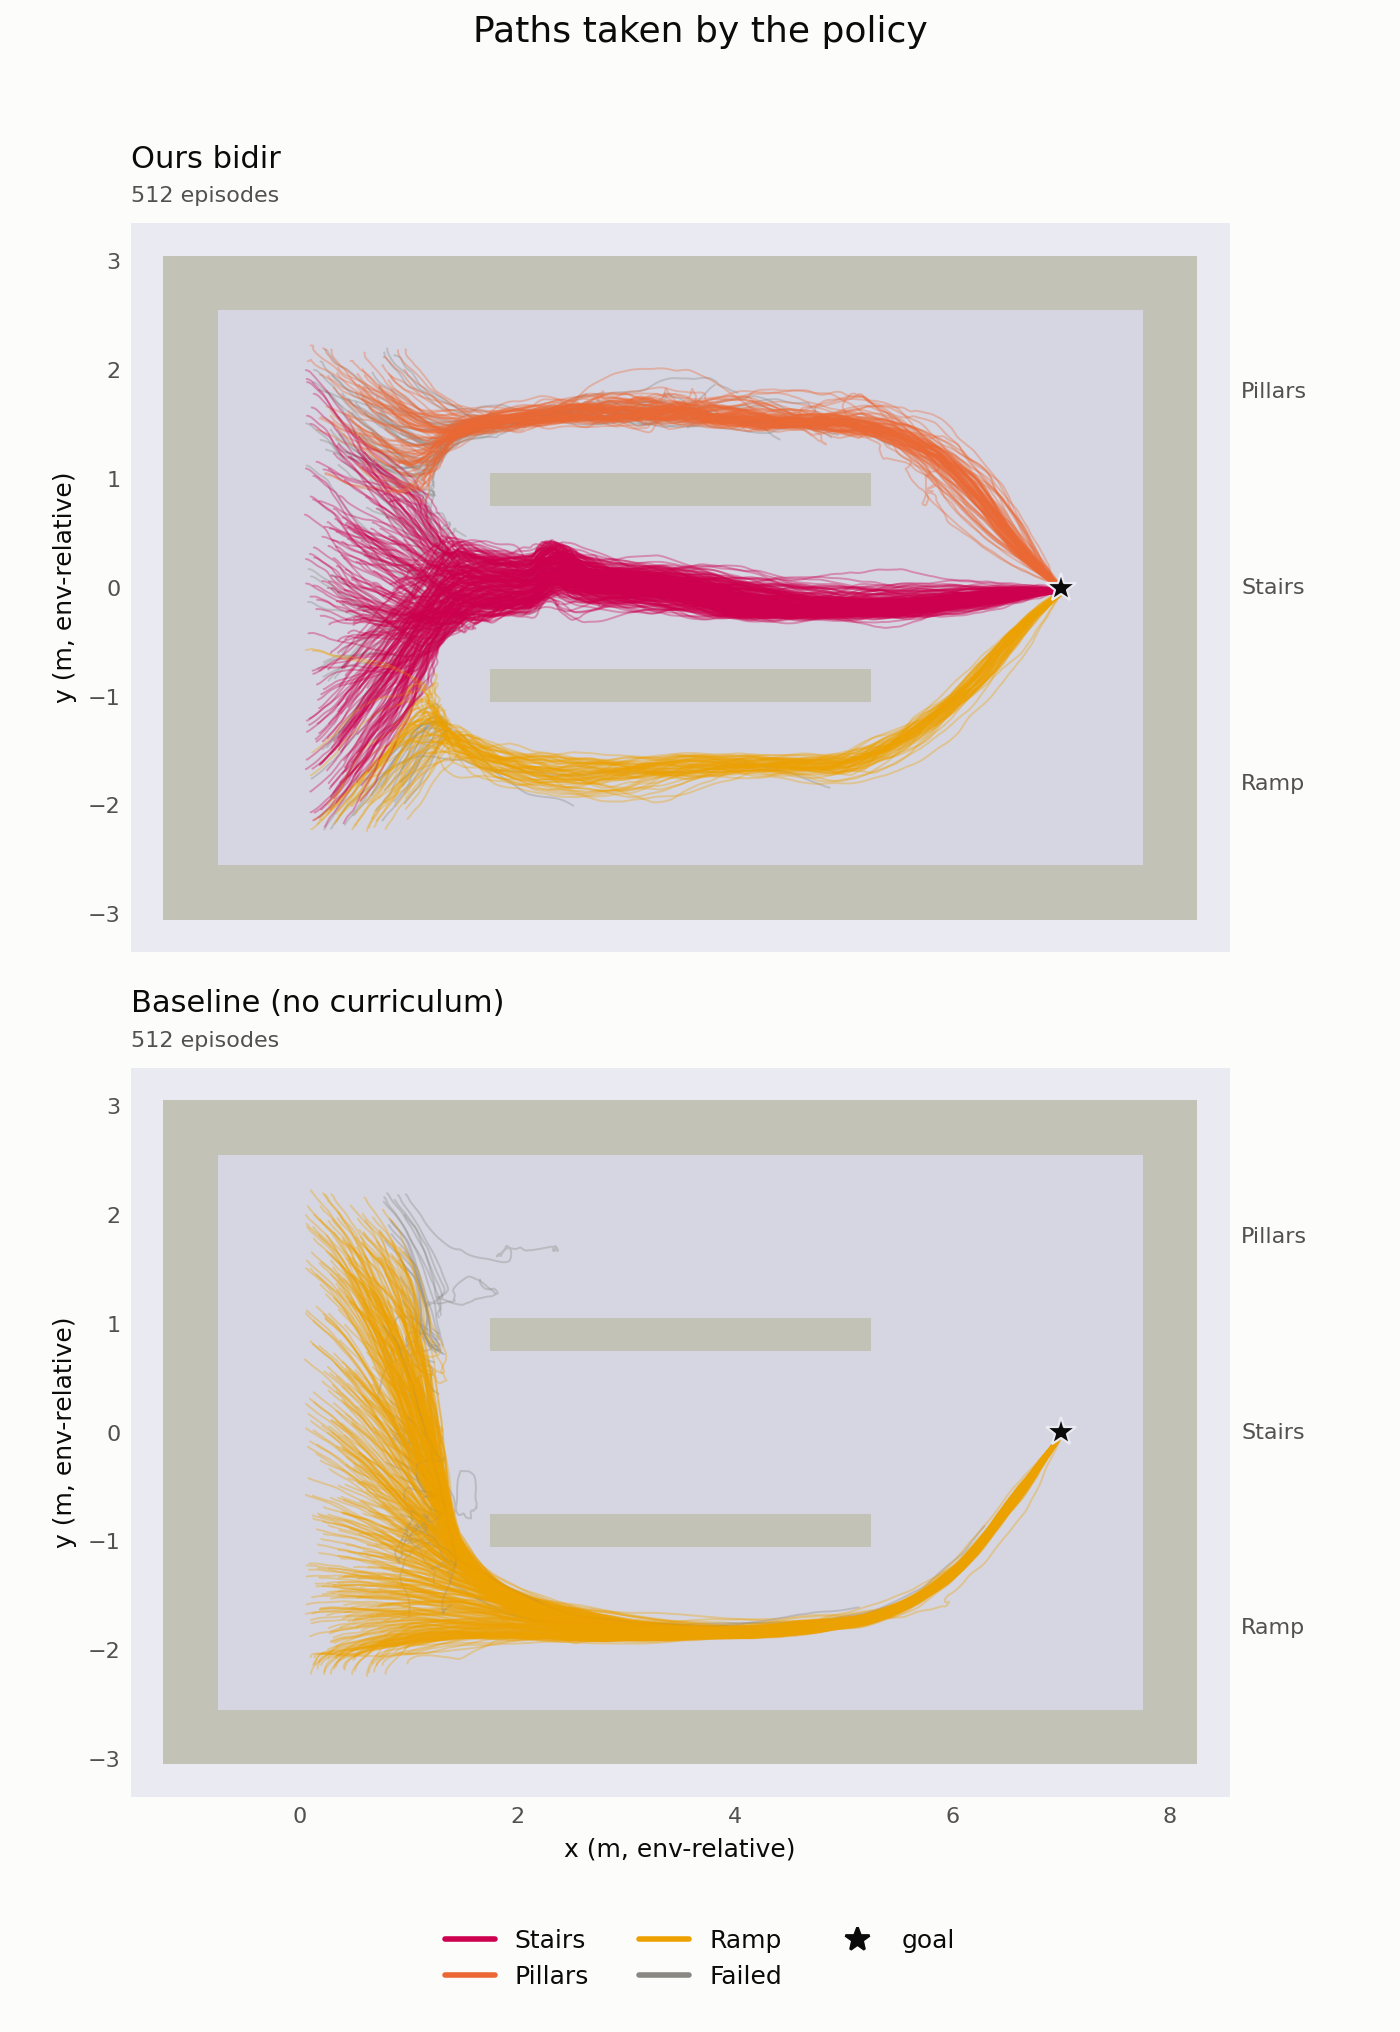
\includegraphics[width=\linewidth]{img/dt/trajectories_model_1999_headline.png}
    \caption{Path diversity on the three-route terrain. PPO without a curriculum collapses onto the ramp, while BVER learns to traverse all three routes.}\label{fig:eval_path_diversity}
\end{wrapfigure}

To answer research question 3, we design a task with three qualitatively different routes from the initial distribution to the goal: a set of stairs in the center, a field of pillars on one side, and a ramp on the other (Figure~\ref{fig:exp_renders_dtsg}). The initial distribution is chosen to span the full width of the terrain, such that each of the three routes is the closest one for roughly a third of the initial states and no route is favored. After training, we roll out both policies from this broad initial distribution and classify every successful episode by the route it takes.

Figure~\ref{fig:eval_path_diversity} shows that PPO without a curriculum collapses onto a single behavior: all successful episodes traverse the ramp, which is the easiest but not necessarily the shortest route, regardless of where the episode starts. Once this route is discovered, exploration of the remaining task space stops, and the policy never learns to climb the stairs or navigate the pillars, even when it is initialized directly in front of them. In contrast, BVER's task-space coverage-driven expansion forces the curriculum to remain active in all regions of the task space, and the resulting policy uses all three routes, choosing the one closest to its initial state. This indicates that task-space coverage promotes more diverse learning outcomes: rather than committing to the first solution it finds, the policy acquires the full set of locomotion skills the terrain affords, which makes it less dependent on any single route being available.

\subsection{Real-World Terrains}\label{sec:exp_real_world}

To show its practical applicability and answer research question 4, we evaluate BVER on four different real-world terrains with the ANYmal D quadrupedal robot in an identical setup to the box climbing task in Section~\ref{sec:exp_main}. We use the same hyperparameters and curriculum settings as in the box climbing task, and choose the task space to roughly cover the terrain area. The four terrains in Figure~\ref{fig:experiment_renders} can be categorized as follows: (1) climbing a freestanding boulder (Figures~\ref{fig:exp_renders_freestanding_boulder_I} and~\ref{fig:exp_renders_freestanding_boulder_II}), (2) traversing over a field of small stones (Figure~\ref{fig:exp_renders_small_rocks}), and (3) ascending a steep rocky slope (Figure~\ref{fig:exp_renders_rocky_ascent}), each requiring different locomotion skills. On the \textit{freestanding boulders} and the \textit{small stone field}, the initial distribution is chosen such that no specific path to the goal is favored and the policy has to find its own path to the goal. Table~\ref{tab:real_world_results} shows that, similar to box climbing, PPO without a curriculum is unable to solve the task, while BVER finds solutions in reasonable time on all four terrains.
% \renewcommand{\arraystretch}{1.3}
\begin{table}[h]
    \centering
    \caption{Training iterations needed to reach a success rate of 95\% on the four real-world terrains.}\label{tab:real_world_results}
    \begin{tabularx}{\linewidth}{@{}rcccc@{}}
        \bf Task    & Freestanding boulder I & Freestanding boulder II & Small stone field & Rocky ascent \\
        \cmidrule{2-5}
        Vanilla PPO & --                     & --                      & --                & --           \\
        BVER        & $1800\pm x$            & $2300\pm x$             & $2500\pm x$       & $3500\pm x$  \\
    \end{tabularx}
\end{table}
% \renewcommand{\arraystretch}{1}

Figure~\ref{fig:scans} shows the explored regions on the \textit{rocky ascent} terrain at different training iterations. The intermediate starts and goals are clustered around their respective roots at the beginning of training, and gradually expand to cover the entire task space as the policy's skill improves. Even though the task space (black/white box) is much larger than the reachable area of the robot, the curriculum is able to find a path to the goal without any prior knowledge of the terrain, showing the effectiveness of the random walks. The even spread of intermediate starts and goals across the task space indicates that the policy has learned to traverse the terrain rather than just solving the target task.
\begin{figure}[h]
    \centering
    \hfill
    \begin{subfigure}[t]{0.24\linewidth}
        \centering
        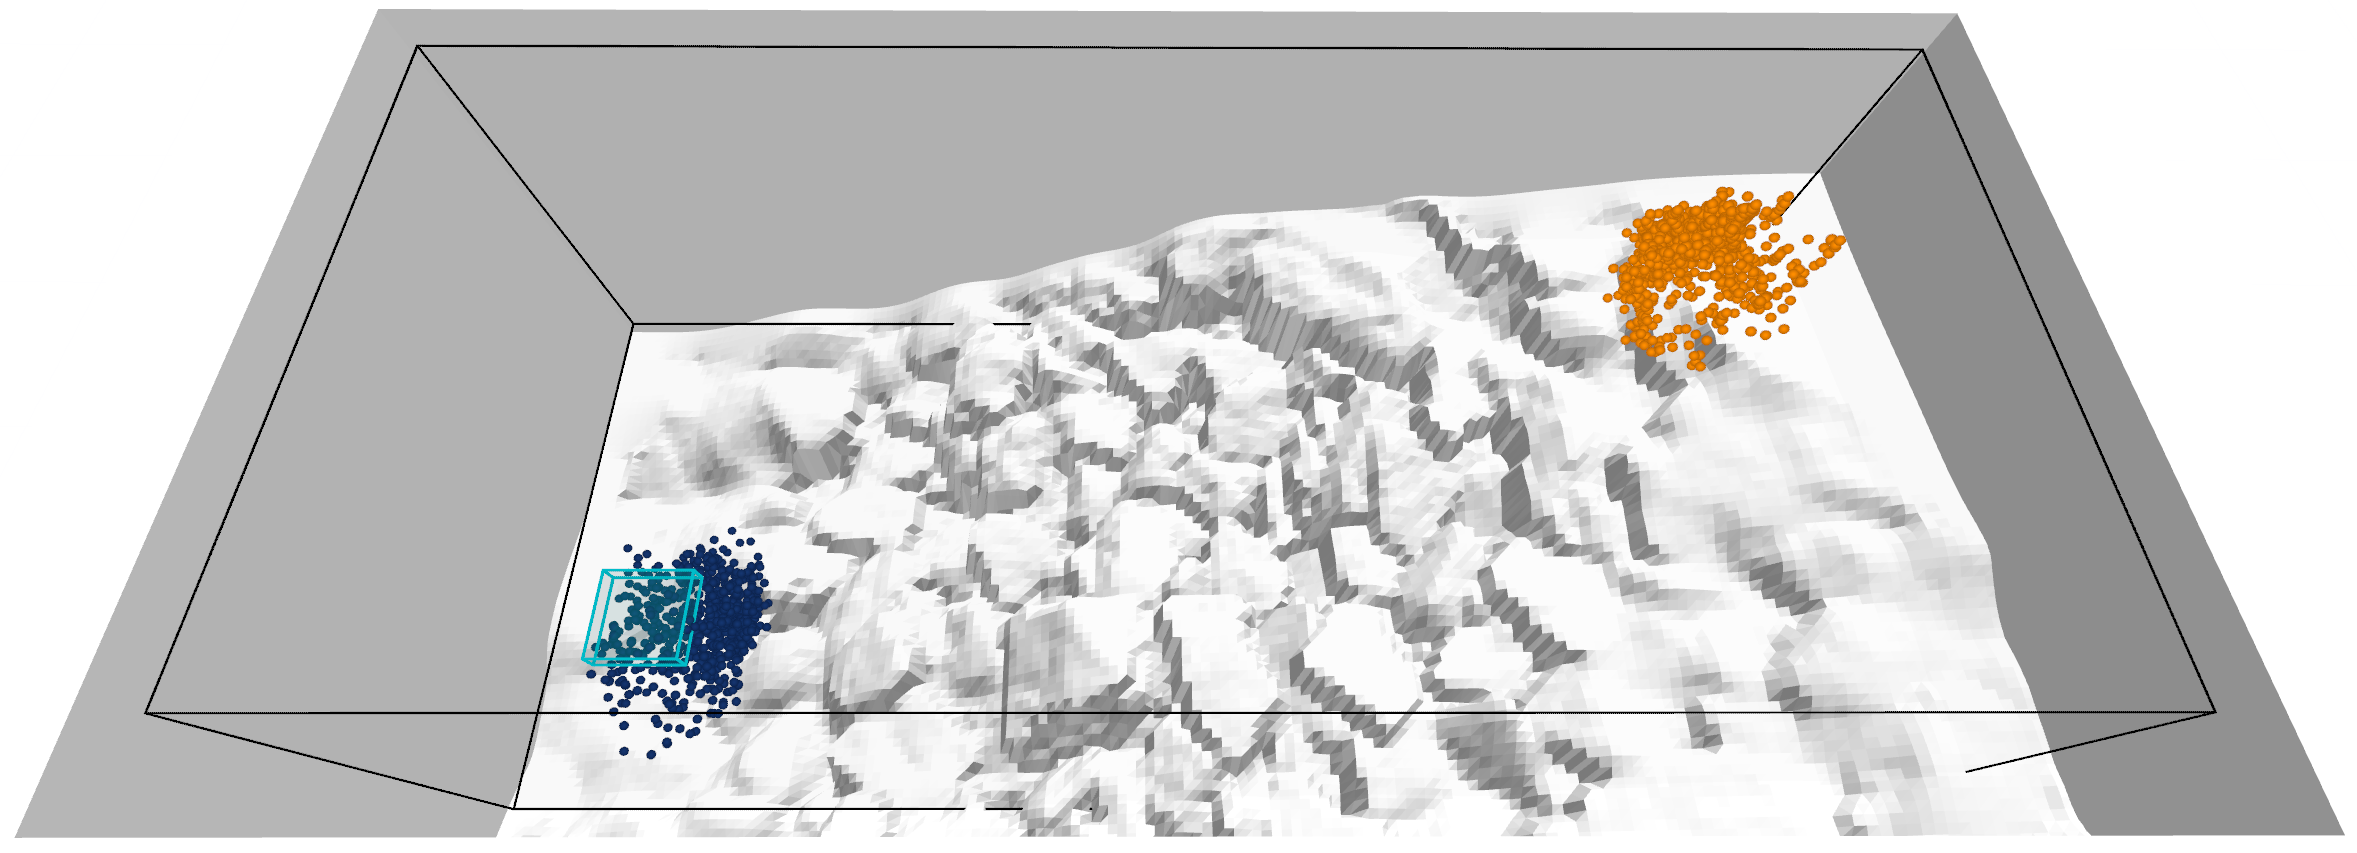
\includegraphics[width=\linewidth]{img/scans/ra_150.png}
        \caption{Iteration 150.}\label{fig:ra_150}
    \end{subfigure}
    \hfill
    \begin{subfigure}[t]{0.24\linewidth}
        \centering
        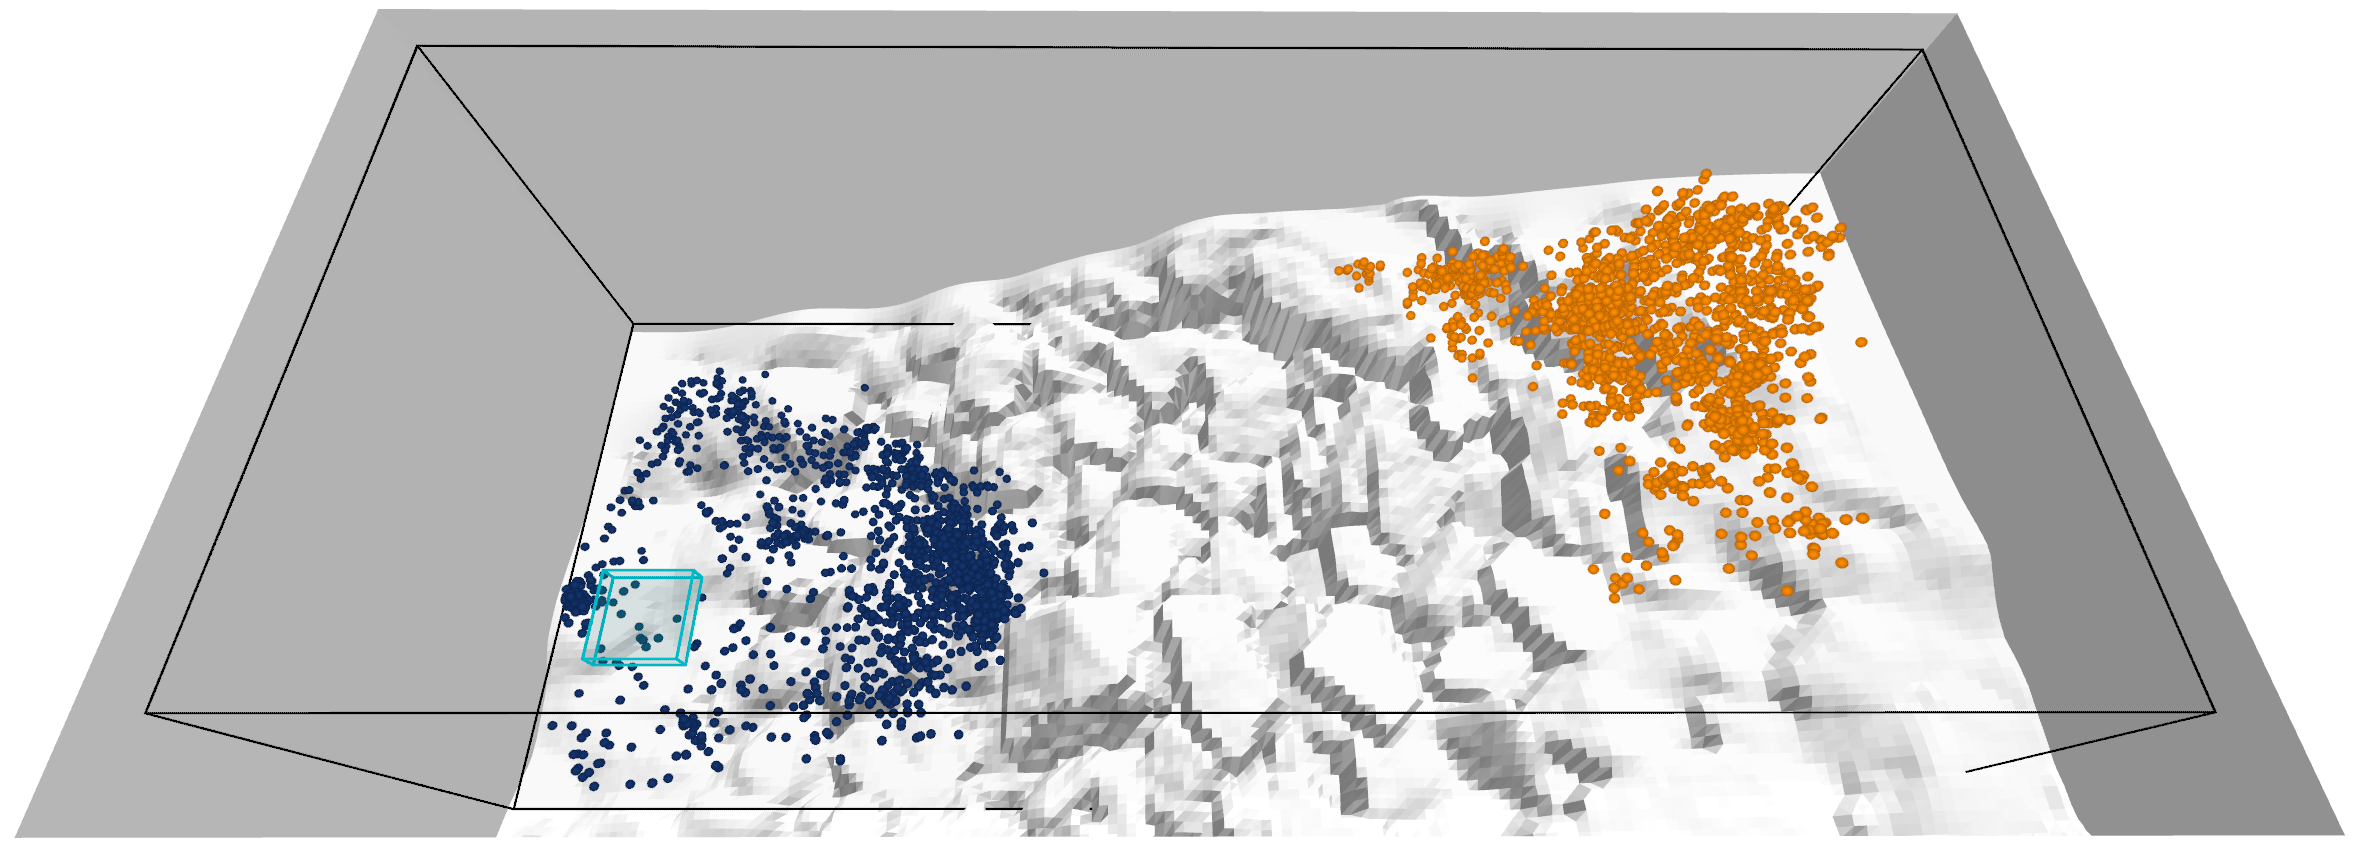
\includegraphics[width=\linewidth]{img/scans/ra_500.png}
        \caption{Iteration 500.}\label{fig:ra_500}
    \end{subfigure}
    \hfill
    \begin{subfigure}[t]{0.24\linewidth}
        \centering
        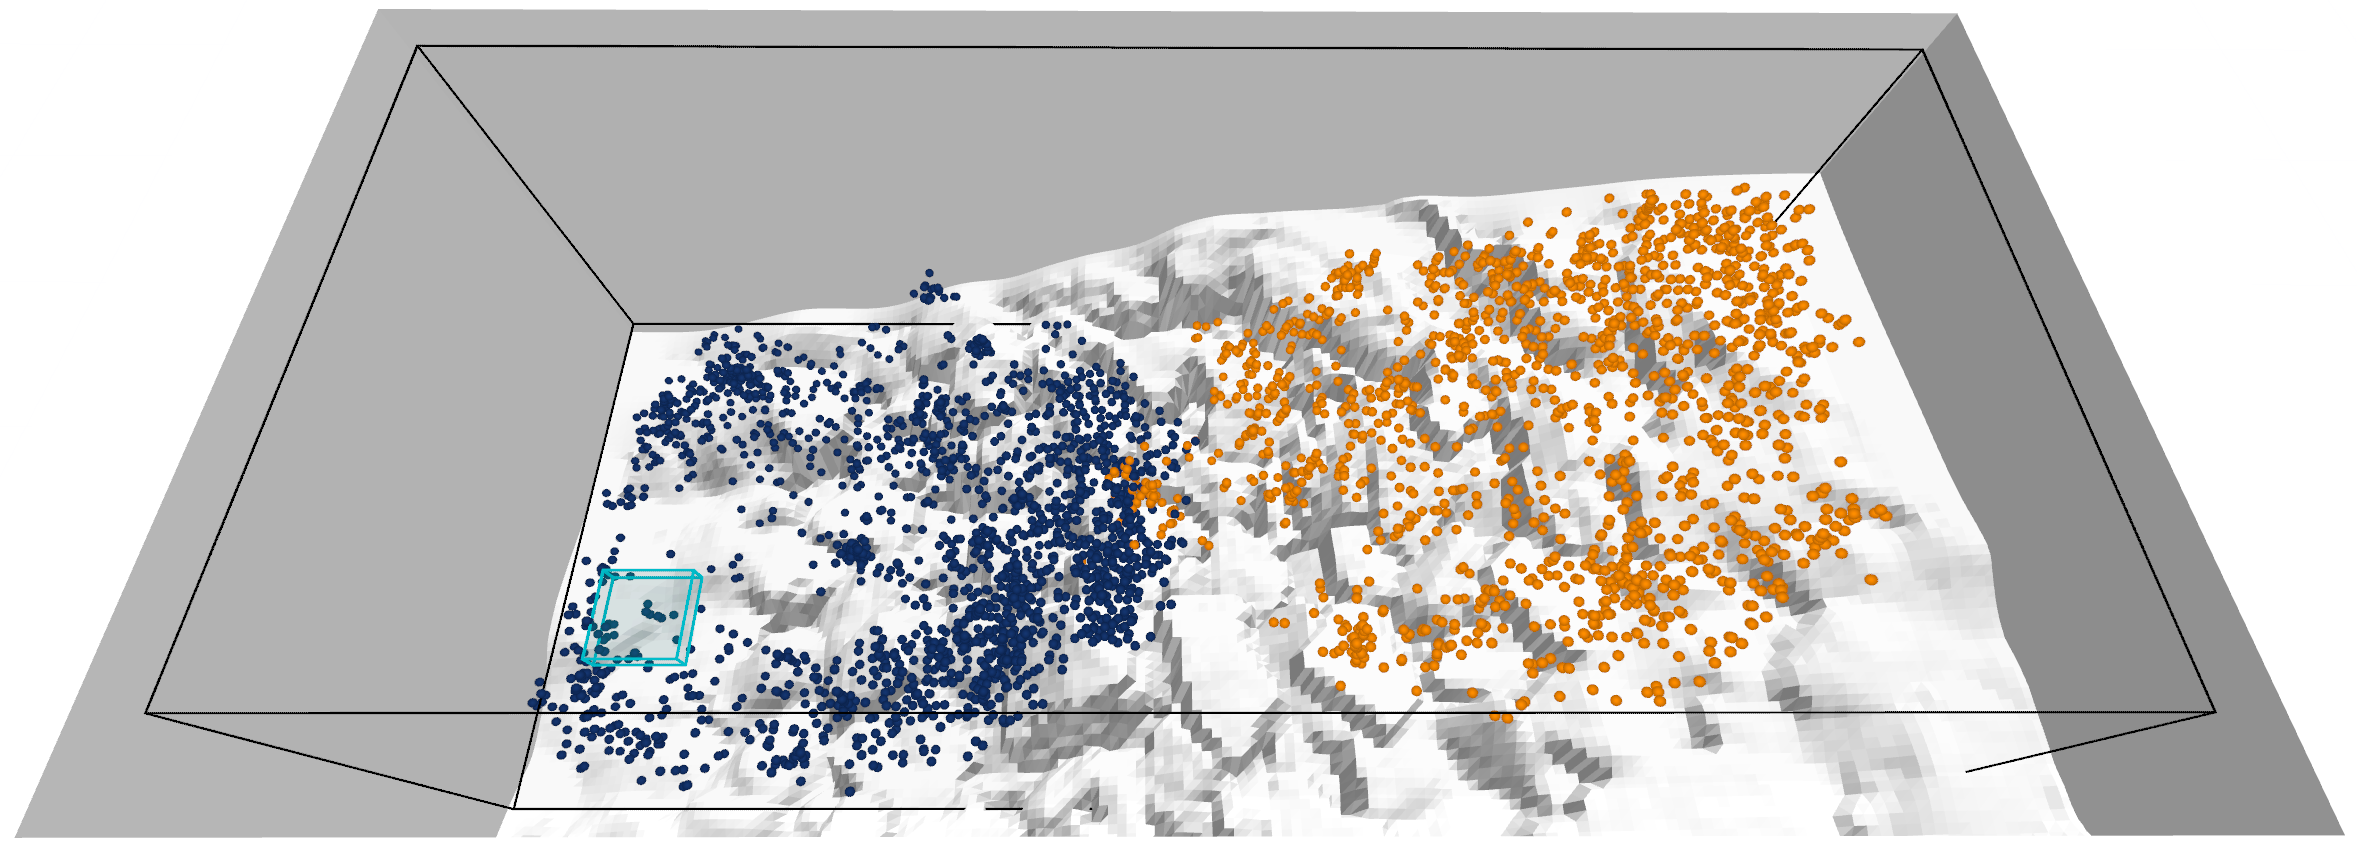
\includegraphics[width=\linewidth]{img/scans/ra_1000.png}
        \caption{Iteration 1000.}\label{fig:ra_1000}
    \end{subfigure}
    \hfill
    \begin{subfigure}[t]{0.24\linewidth}
        \centering
        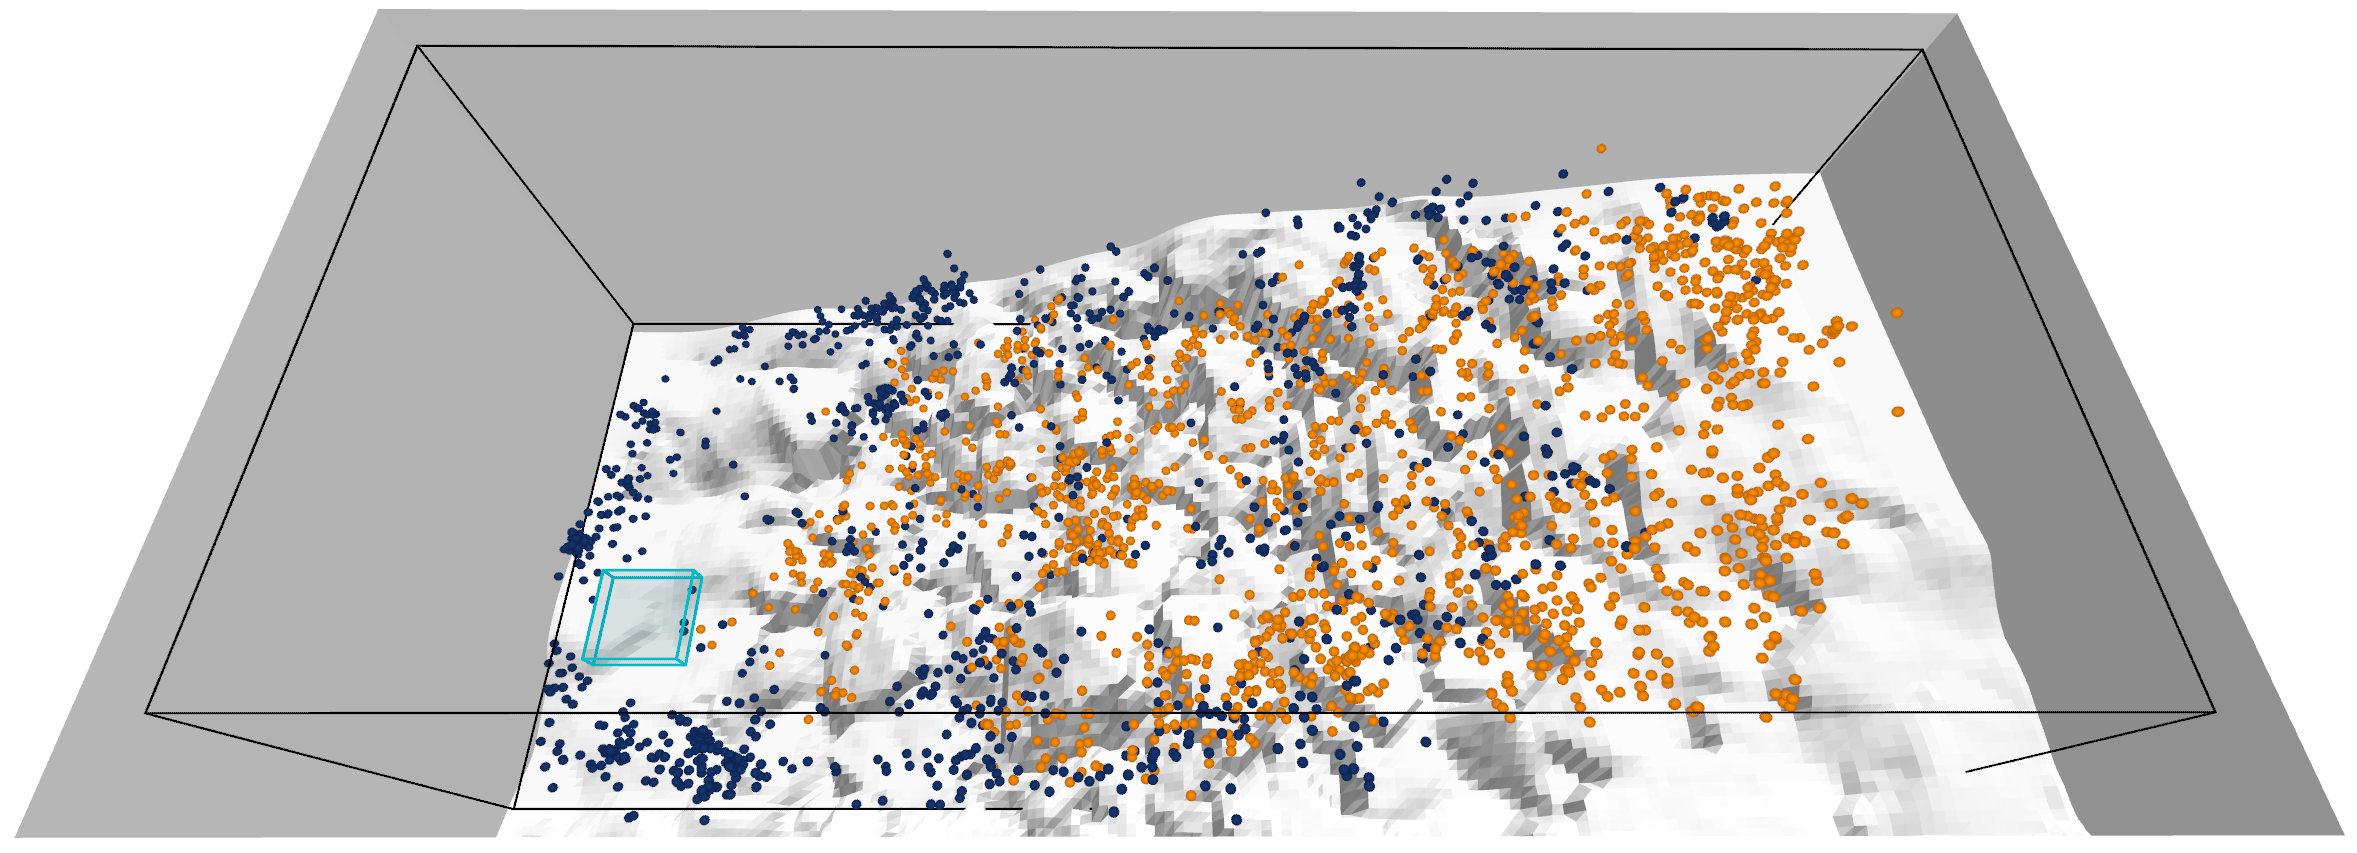
\includegraphics[width=\linewidth]{img/scans/ra_2000.png}
        \caption{Iteration 2000.}\label{fig:ra_2000}
    \end{subfigure}
    \hfill\strut{}
    \caption{Samples of the explored regions on the \textit{rocky ascent} terrain at different training iterations. {\color{blue} Blue} indicates the intermediate goals (forwards expansion), {\color{orange} orange} indicates the intermediate starts (backwards expansion), {\color{cyan}cyan} indicates the initial distribution, and the black/white box represents the task space.}\label{fig:scans}
\end{figure}
\subsection{Generalization to Different Domains: Manipulation Tasks}\label{sec:exp_manipulation}

todo
\begin{wrapfigure}{r}{0.24\linewidth}
    \centering
    \vspace{-\baselineskip}
    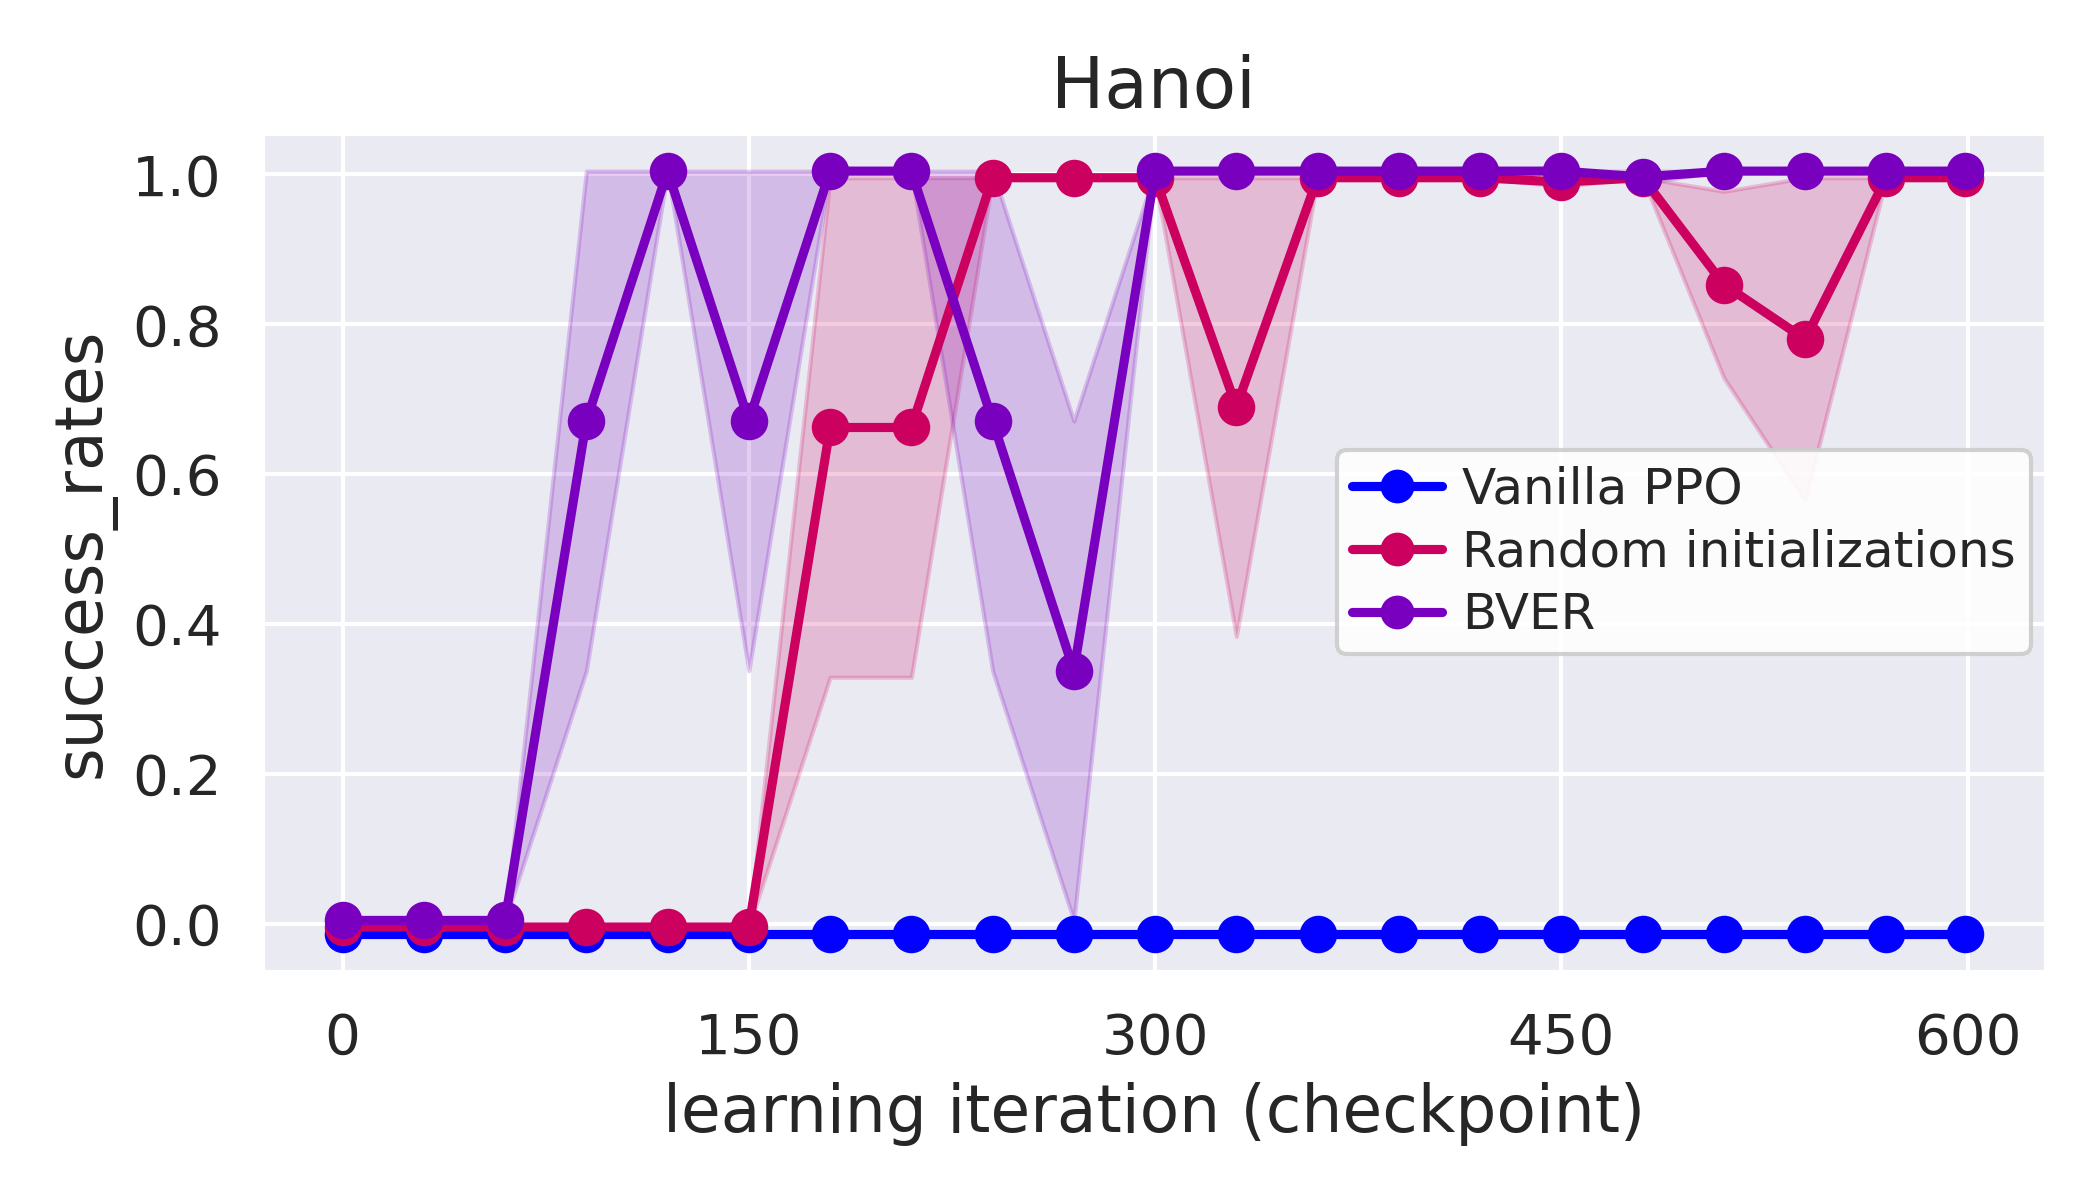
\includegraphics[width=\linewidth]{img/manipulation/eval_comparison_hanoi_bench.png}
    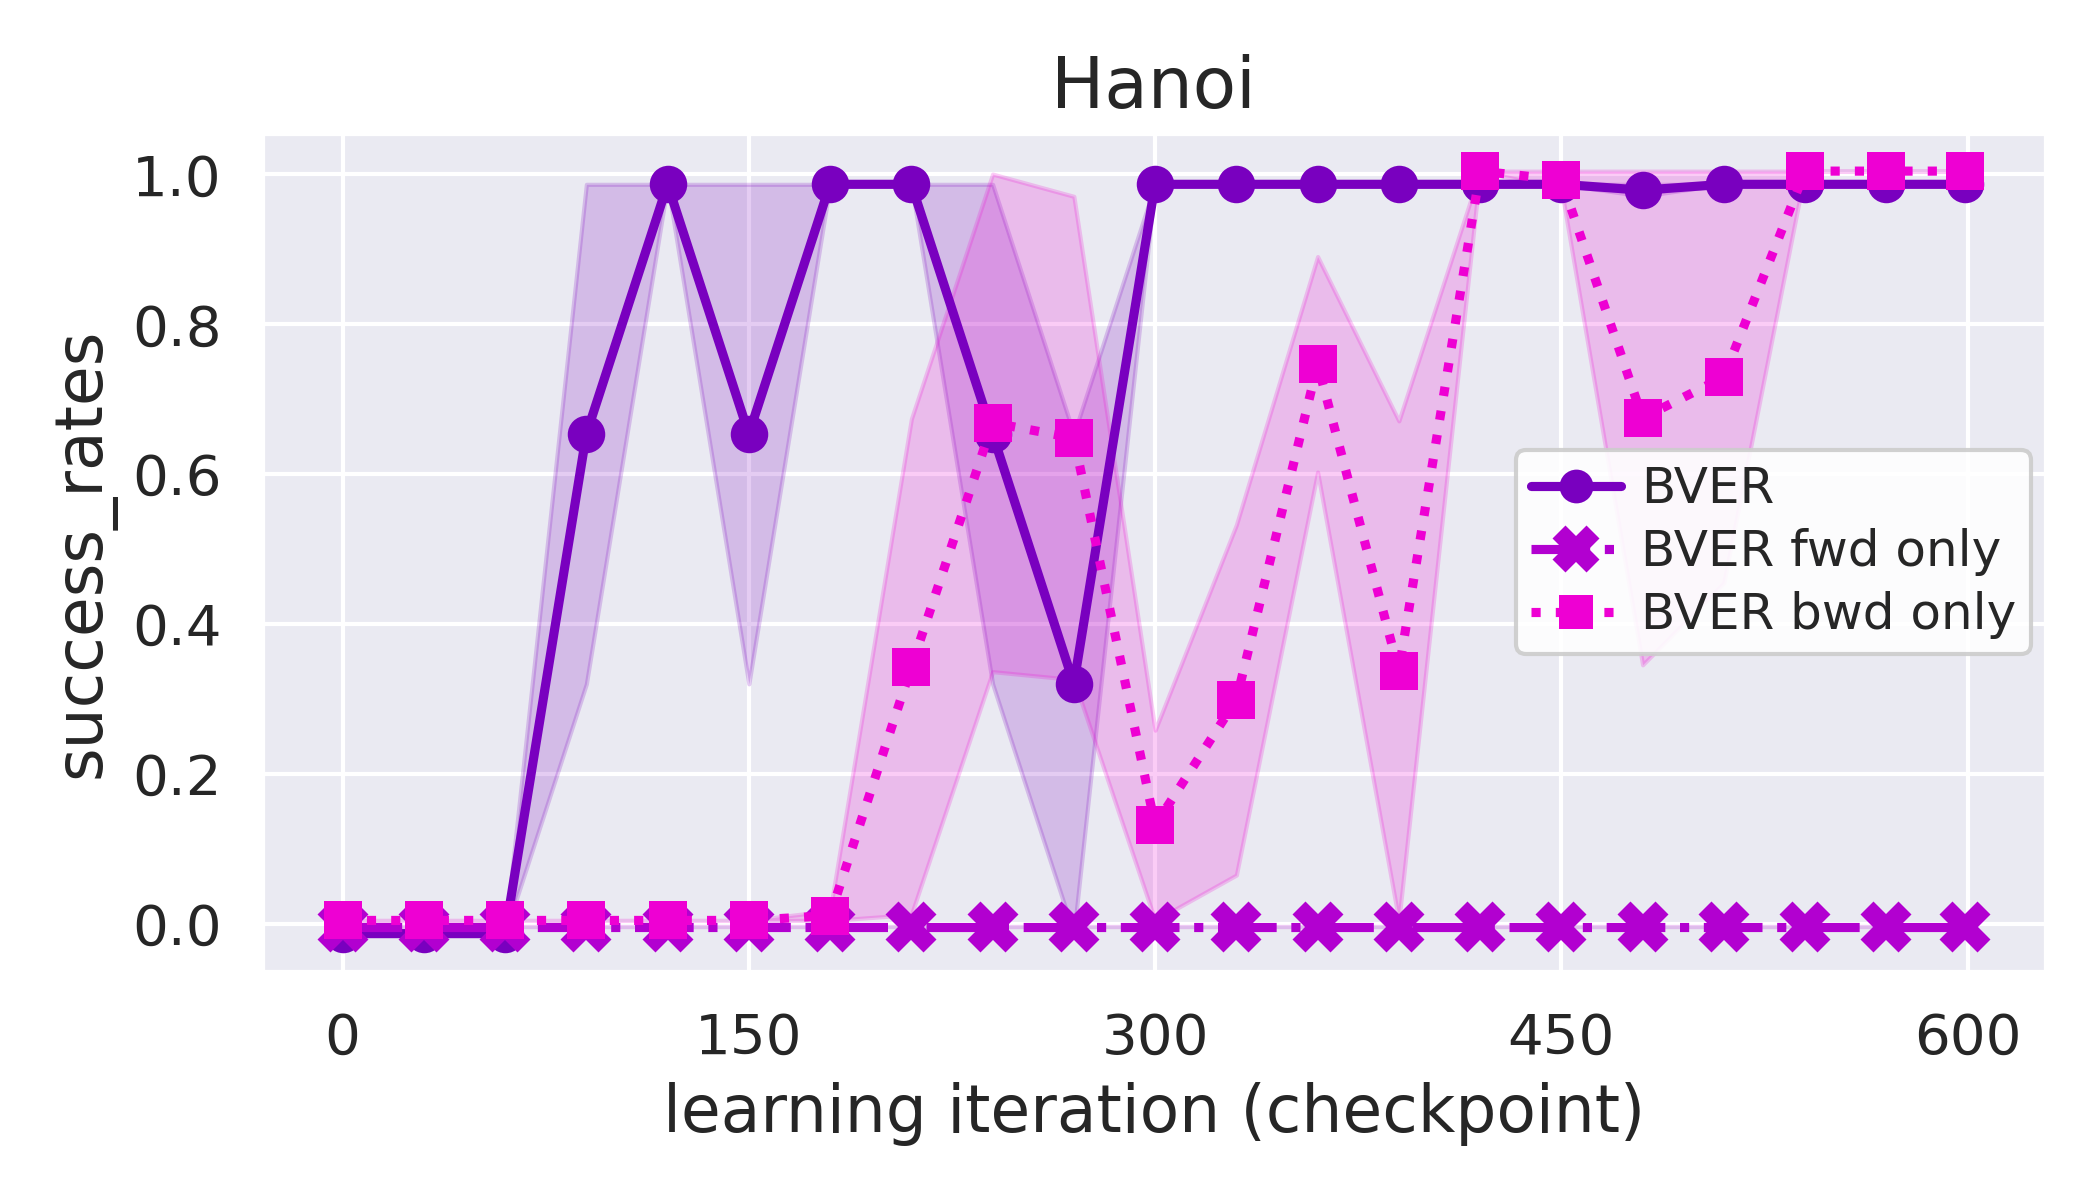
\includegraphics[width=\linewidth]{img/manipulation/eval_comparison_hanoi_abl_dir.png}
    \caption{Top row shows the benchmark results, and the bottom row shows the ablation results.}\label{fig:hanoi_p12}
\end{wrapfigure}